%!TEX encoding = UTF-8 Unicode
%!TEX program = xelatex


\documentclass[a4paper, twoside,12pt]{ctexbook}%{report}
\usepackage[utf8]{inputenc}
\usepackage{indentfirst}
\setlength{\parindent}{2em}
\usepackage{pdfpages}
\usepackage{float}
\usepackage{longtable}
\usepackage{diagbox} 
\usepackage{booktabs}%设置表格粗线
\usepackage{subfigure}
\usepackage{multirow}
\usepackage{listings}
\usepackage{multicol}
\usepackage{color}

%----------------------font-------------------------------------------
\usepackage{fontspec}

%\setmainfont{Times New Roman} 
%--------------------------------------------------------------
\usepackage{xcolor, colortbl}%table color
\usepackage[margin=1in, showframe=false]{geometry}
\definecolor{Gray}{gray}{0.85}
\definecolor{LightCyan}{rgb}{0.88,1,1}
%--------------------------------------------------------------
%\usepackage{titletoc}
%\usepackage{titlesec}
%\titleformat{\section}{\centering\LARGE\bfseries}{Chapter \arabic{section}}{11pt}{}
%\titleformat{\subsection}{\large\bfseries}{\arabic{section}.\arabic{subsection}}{1em}{}

\renewcommand{\theequation}%
  {\arabic{section}.\arabic{equation}}
%\usepackage{amsmath}
%\numberwithin{equation}{section}

\renewcommand{\thefigure}
  {\arabic{section}.\arabic{figure}}
\renewcommand{\thetable}
  {\arabic{section}.\arabic{table}}

\usepackage{amsmath} %数学公式
\usepackage{mathtools}
\usepackage{bm}%专门处理数学粗体的bm宏包
%\usepackage{extarrows}
\usepackage{enumerate}
%-----------------------------------------------------------------
\usepackage{url}
\usepackage{cite}
\usepackage[colorlinks, linkcolor=blue, anchorcolor=blue, urlcolor=blue, citecolor=blue, breaklinks=true]{hyperref} 
\usepackage[square, numbers, sort&compress]{natbib} % 上标,加中括号,编号,将8,9,10改为8-10
\usepackage[hypcap=false]{caption}

%----------------------------------------------------------------------------
\usepackage{graphicx}% Include figure files
\graphicspath{{figure/}}%directory of my plots
%\usepackage{placeins}
%-----------------------------------------------------------------------------

\usepackage{ctex}   %  添加中文支持

%\renewcommand{\thefigure}{\thechapter{}.\arabic{figure}}
%\renewcommand{\thetable}{\thechapter{}.\arabic{table}}
\renewcommand{\theequation}{\thechapter{}.\arabic{equation}}
\renewcommand{\figurename}{Fig.}
\def\figureautorefname{Fig.}
\renewcommand{\tablename}{Tab.}
\def\tableautorefname{Tab.}
\def\equationautorefname{Eq.}

\def\figurename{图}%
\def\tablename{表}%
\renewcommand{\theequation}{\thesection.\arabic{equation}}%
\renewcommand{\thefigure}{\thesection.\arabic{figure}}%
\renewcommand{\thetable}{\thesection.\arabic{table}}%
\renewcommand{\baselinestretch}{1.25}
\baselineskip 19pt \cleardoublepage

%------------------------------------------------------------------------------
\usepackage{fancyhdr}
\pagestyle{fancy}
\fancyhead{} % clear all fields 
\fancyfoot{} % clear all fields 
\fancyhead[LO]{\leftmark}
\fancyhead[RE]{\rightmark}
\fancyhead[LE,RO]{\thepage} 
%\fancyhead[LE, RO]{\includegraphics[scale=0.1]{figure/ccnu_logo.png}} 
%\fancyfoot[CO]{\thepage} 
%==================================================
\newcommand{\thesisTitle}{The study of the Chiral Magnetic Effect in Relativistic Heavy Ion Collisions at STAR}
\newcommand{\yourName}{Yufu Lin}
\newcommand{\yourCollege}{College of Physical Science and Technology}
\newcommand{\yourSchool}{Central China Normal University}
\newcommand{\yourYear}{2021}
\newcommand{\yourMonth}{Jun.}

\newcommand{\npart}{$\langle N_{part} \rangle\, $}
\newcommand{\sNN}{$\sqrt{s_{\mathrm{NN}}}\, $}
\newcommand{\egy}{$\sqrt{s_{\mathrm{NN}}} =  $ 7.7, 11.5, 14.5, 19.6, 27, 39, 54.4, 62.4 and 200 GeV}
\newcommand{\egyfive}{$\sqrt{s_{\mathrm{NN}}} = $ 7.7, 11.5, 14.5, 19.6, 27, 39, 62.4 and 200 GeV}
\newcommand{\egyfxt}{$\sqrt{s_{\mathrm{NN}}} = $ 4.5, 7.7, 11.5, 14.5, 19.6, 27, 39, 54.4, 62.4 and 200 GeV}
\newcommand{\egycucu}{$\sqrt{s_{\mathrm{NN}}} =  $ 22.4, 62.4 and 200 GeV}

\newcommand{\allSys}{in Au+Au collisions at $\sqrt{s_{\mathrm{NN}}} = 7.7 - $200 GeV, in FXT collisions at $\sqrt{s_{\mathrm{NN}}} =  $ 4.5 GeV and in Cu$+$Cu collisions at $\sqrt{s_{\mathrm{NN}}} =  $ 22.4, 62.4 and 200 GeV\,}

\newcommand{\allpt}{$0.4 < p_{\mathrm{T}} < 2.0 \, (\mathrm{GeV}/c)\,$}
\newcommand{\lowpt}{$0.4  <p_{\mathrm{T}} < 0.8 \, (\mathrm{GeV}/c)\,$}
\newcommand{\highpt}{$0.8 < p_{\mathrm{T}} < 2.0 \, (\mathrm{GeV}/c)\,$}

\newcommand{\cum}{$C_1, C_2, C_3$ and $C_4\, $}
\newcommand{\ratio}{$C_{2}/C_{1}, C_{3}/C_{2}$ and $C_{4}/C_{2}\, $}
\newcommand{\cumratio}{$C_{1}, C_{2}, C_{3}, C_{4}, C_{2}/C_{1}, C_{3}/C_{2}$ and $C_{4}/C_{2}\, $}

\newcommand{\pt}{$p_{\mathrm{T}}$}
\newcommand{\dEdx}{$d\mathrm{E}/dx$}
\newcommand{\MeVc}{$\mathrm{MeV}/c$}
\newcommand{\GeVc}{$\mathrm{GeV}/c$}
%\newcommand{\corrfun}{$\kappa_1, \kappa_2, \kappa_3$ and $\kappa_4\, $}
\newcommand{\corrfun}{$\kappa_{2}/\kappa_{1}, \kappa_{3}/\kappa_{1}$ and $ \kappa_{4}/\kappa_{1}$}

\newcommand{\tofm}{nTofmatch\,}
\newcommand{\btofm}{Beta\_eta1\,}

\renewcommand{\vec}{\boldsymbol }
\newcommand{\rap}{Y}
\newcommand{\qw}{Q_\mathrm{w}}
\newcommand{\nw}{n_\mathrm{w}}
\newcommand{\qp}{Q_\mathrm{p}}
\newcommand{\nt}{N_\mathrm{t}}
\newcommand{\na}{N_\mathrm{a}}
\newcommand{\nb}{N_\mathrm{b}}
\newcommand{\dt}{\Delta_\mathrm{t}}


\newcommand{\gevc}{$\mathrm{GeV}/c$}
\newcommand{\gev}{$\mathrm{GeV}$}
\newcommand{\rlab}{$r_{\mathrm{lab}}$}
\newcommand{\rrest}{$r_{\mathrm{rest}}$}
\newcommand{\rb}{$r_{\mathrm{B}}$}
\newcommand{\ns}{$n_5/s$}


%---------------------------------------------------------------------------------------------
%=======================================================
\graphicspath{{figures/}}


\begin{document}
\date{} 
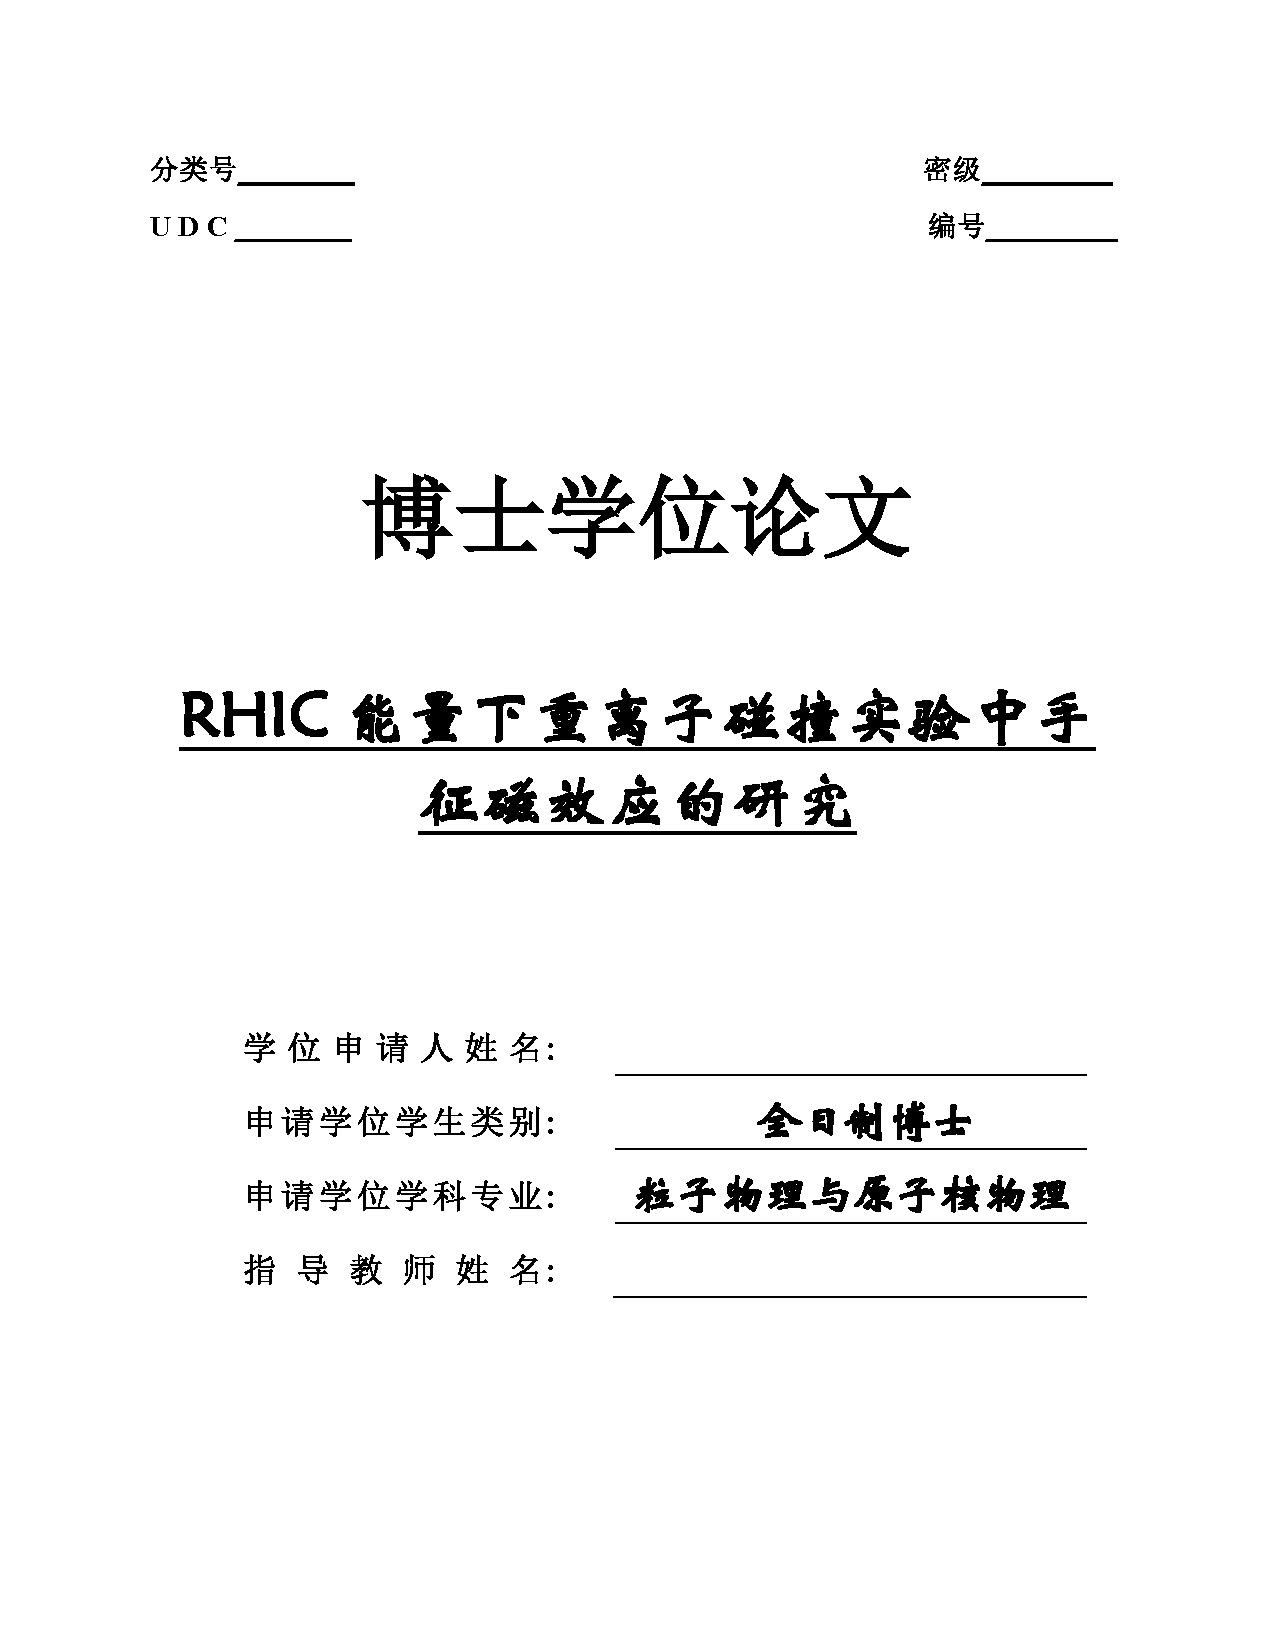
\includepdf[pages={1}]{Chapter/cover2.pdf}
%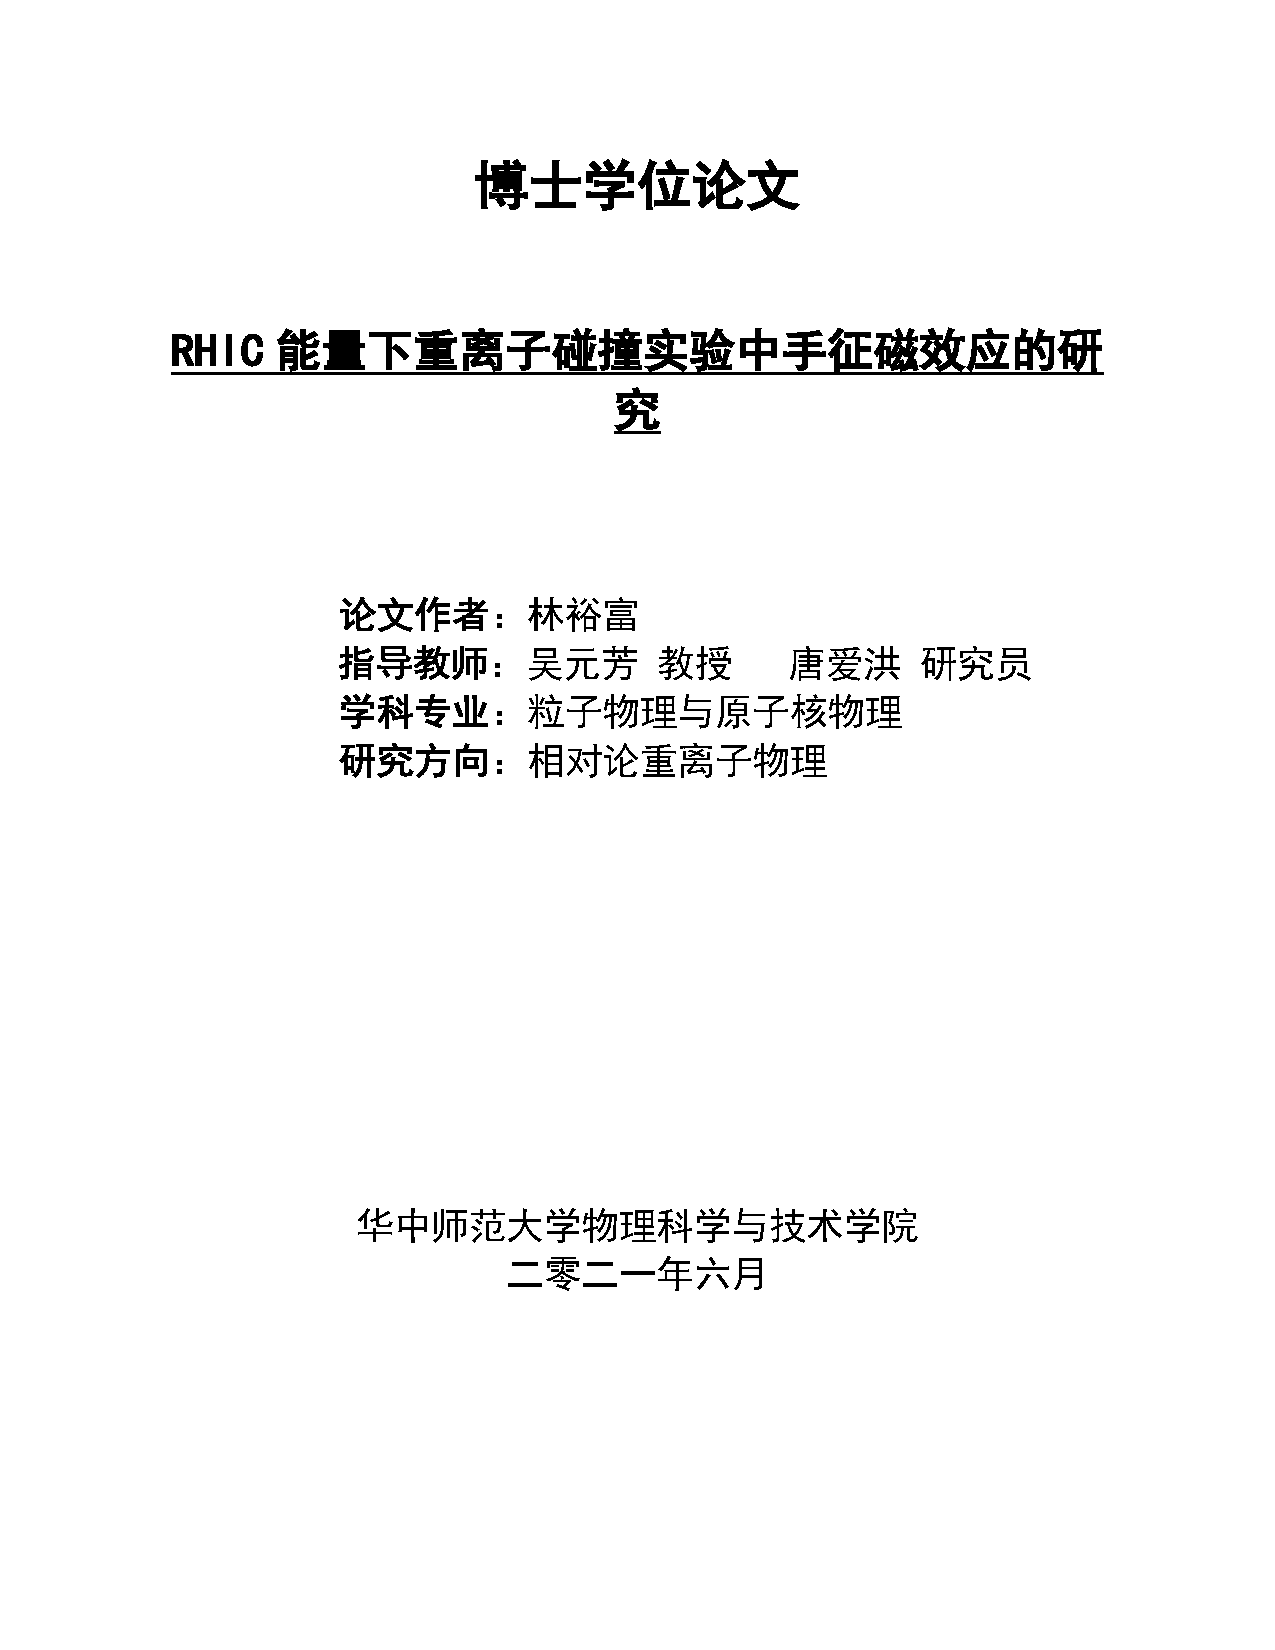
\includepdf[pages={1}]{Chapter/title_CN.pdf}
%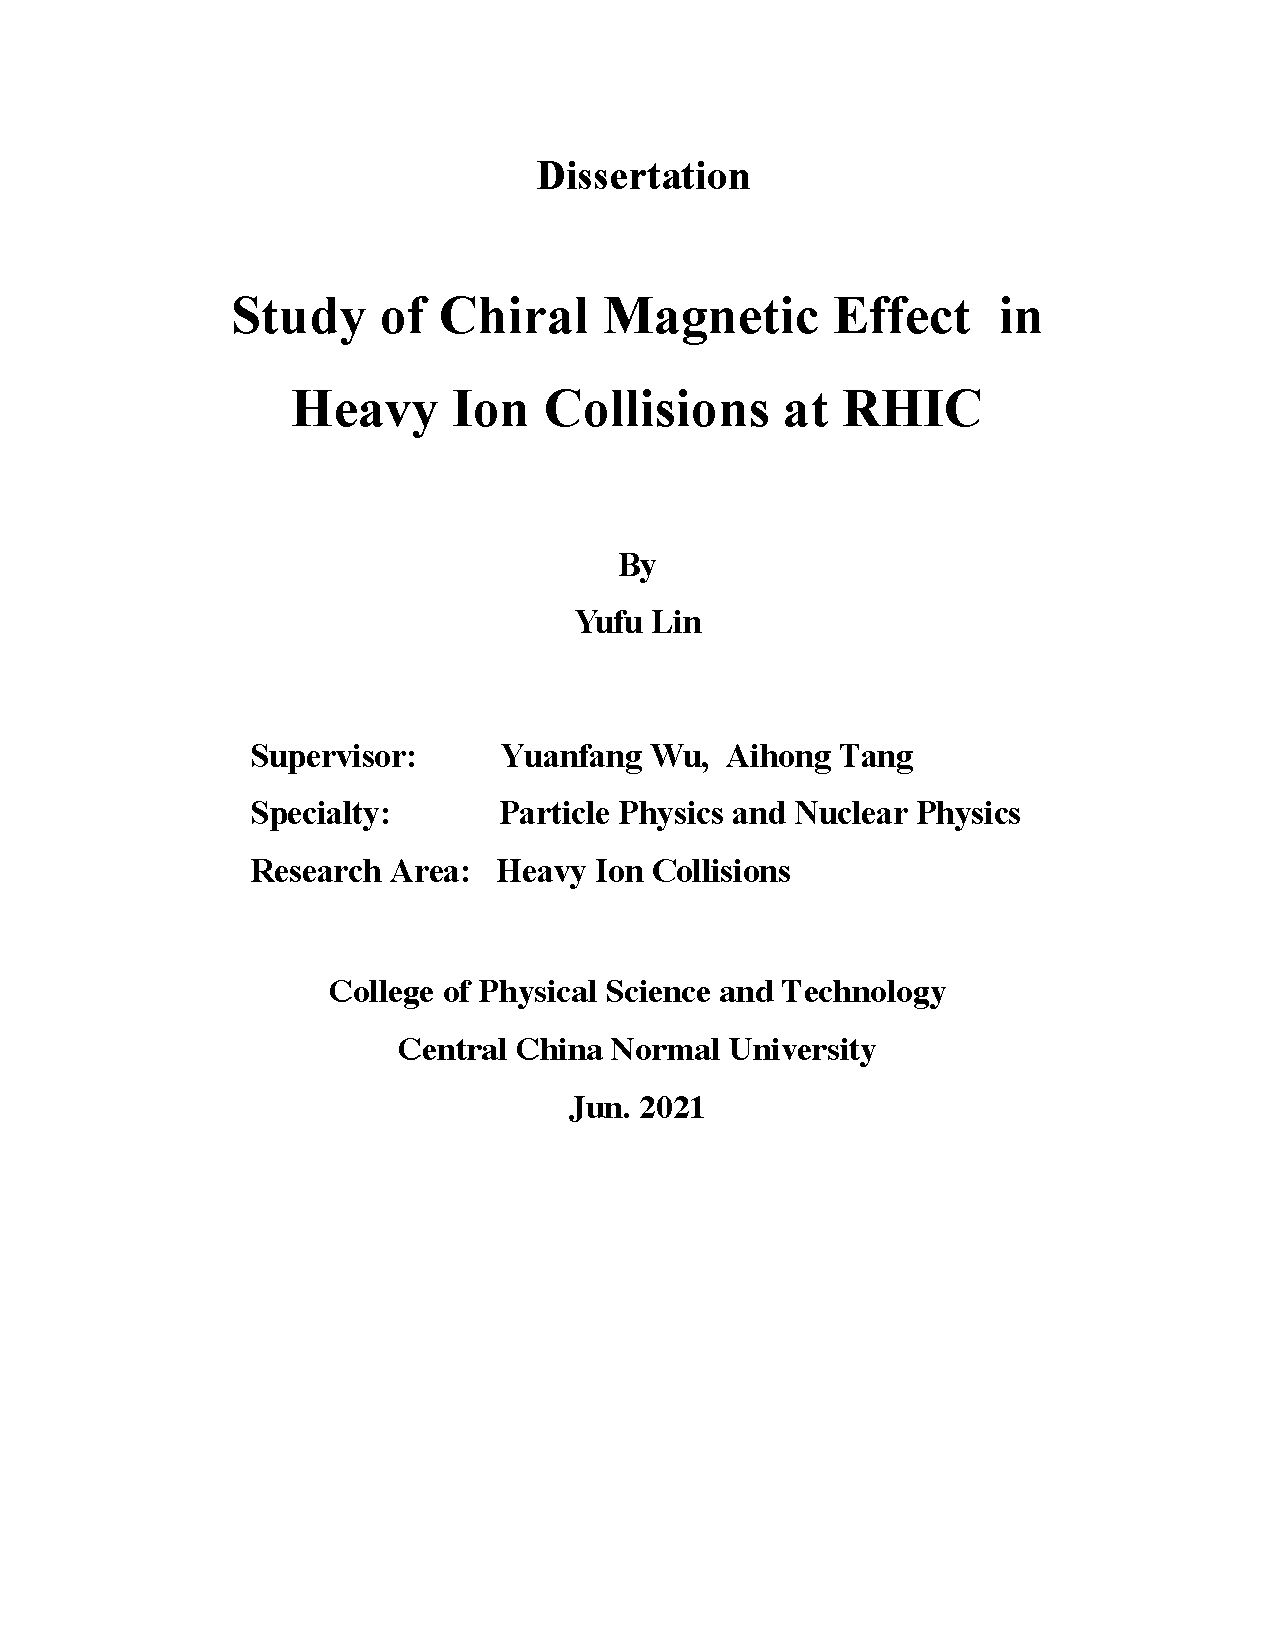
\includepdf[pages={1}]{Chapter/title_EN.pdf}
%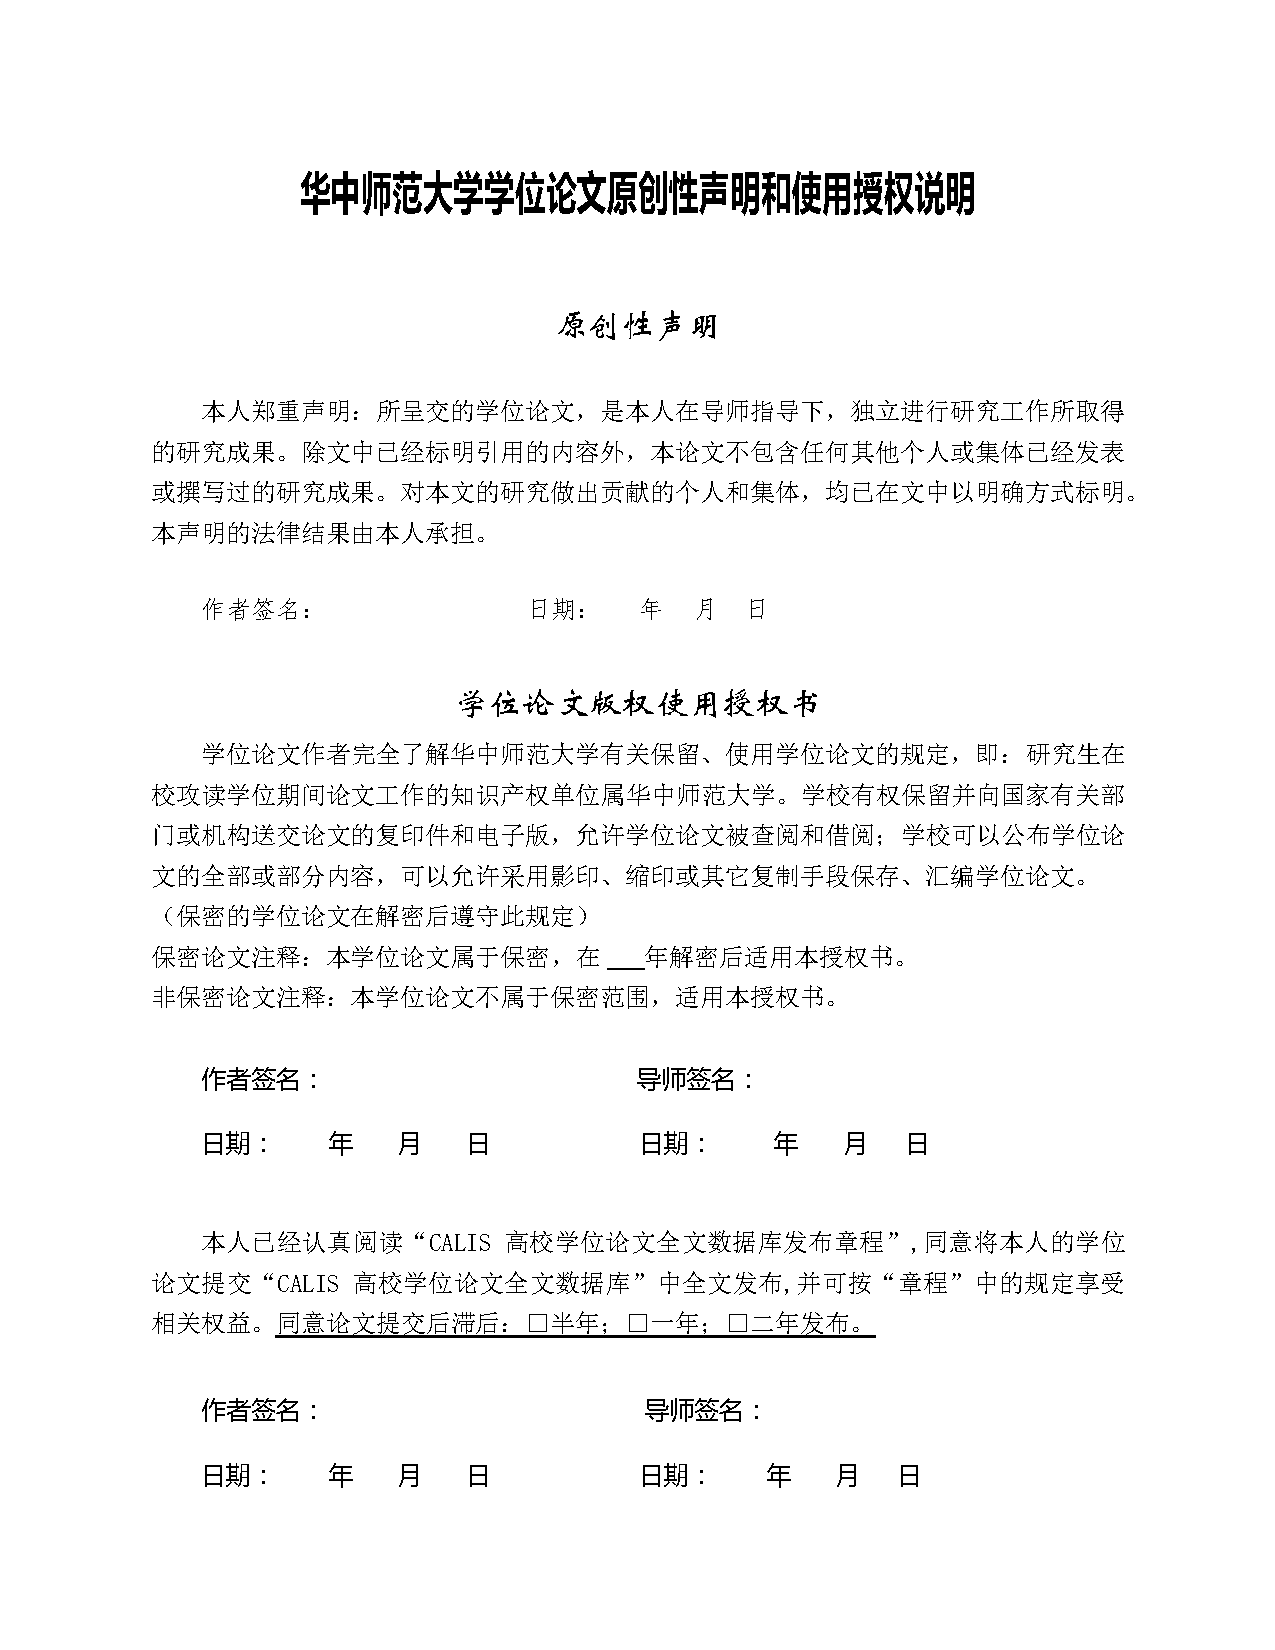
\includepdf[pages={1}]{Chapter/declaration_CN.pdf}
%=======================================================

\newpage
\pagenumbering{roman}
%=======================================================
%---------------------------------------------------------------------------------------------
%=======================================================
%   Abstract 


\setcounter{section}{0}
%==========================================



\chapter*{摘要}

实验研究显示,在高能重离子碰撞中产生了高温高密强耦合的新物质形态——夸克胶子等离子体(Quak-Gluon Plasma, QGP)。在美国布鲁克海文国家实验室建造的相对论重离子对撞机(RHIC)是主要用来研究夸克胶子等离子体的性质及量子色动力学相图的实验装置。在非对心碰撞中,夸克胶子团在旁观质子的运动而产生的极强磁场的作用下,在磁场方向上会出现电荷分离的效应,这就是所谓的手征磁效应(Chiral Magnetic Effect, CME)。实验上致力于寻找重离子碰撞中的手征磁效应已经十多年,但目前为止还没有明确的结论证实它的存在。其中最主要的难点在于手征磁效应研究中很难有效的扣除背景,特别是与共振态的椭圆流相关的背景,它们也会在垂直于磁场的方向上产生类似的分离效应。

最近电荷平衡函数法(Signed Balance Function)被认为可以作为寻找CME的探针,它是基于检验由磁场作用而导致的粒子对横动量差的净取向在垂直、平行反应平面两个方向上起伏的区别而提出来的新方法。在这个方法中提出了一对观测量:$r_{\mathrm{rest}}$ 和$R_{\mathrm{B}}$,这两者对信号、背景的反应不一样。即$r_{\mathrm{rest}}$ 在包含共振态的椭圆流等背景等情况下会增大,而此时
$R_{\mathrm{B}}$会被压低。如果这两个观测量都大于1,那么这种情况就很有可能存在CME。本文利用Toy模型、多相输运模型模型(AMPT)和
异常粘滞流体动力学模型(EBE-AVFD)对该方法的有效性进行了进一步的检验。结果表明该方法通过对$r_{\mathrm{rest}}$ 和$R_{\mathrm{B}}$的结果对比,可以很好的鉴别信号与背景。接下来本文对实验上用于寻找CME的三个基本的方法进行了研究,通过比较它们的核心组成部分发现是相互关联的,它们的核心组成部分在模型中的结果也表明它们对信号和背景的反应是相似的,在此基础上我们认为这三种方法并没有明显的区别。
本文还利用电荷平衡函数法对STAR实验中所采集的Au+Au200GeV 的数据进行研究,$r_{\mathrm{rest}}$,  $r_{\mathrm{lab}}$ 和 $R_{\mathrm{B}}$ 在所有中心度中都大于1,且大于EBE-AVFD模型中没有手征磁效应信号时的结果。这一结果很难被解释为只有背景存在的情况下导致的。

为了能够更好的扣除背景的贡献, 在RHIC的螺线管径迹探测器(The Solenoidal Tracker At RHIC,STAR)实验组进行了同质异荷数对撞实验(Isobar collision),目前正在进行数据分析。这两个Isobar系统分别是:钌($^{96}_{44}$Ru + $^{96}_{44}$Ru)和锆($^{96}_{40}$Zr + $^{96}_{40}$Zr),因为它们具有相同数量的核子数但具有不同的质子数,这就使得两对撞系统会有相同的背景(椭圆流)而具有不同的磁场大小,即两个碰撞系统的CME信号的大小不同。两个Isobar系统通过控制背景不变而改变信号的大小这样就得到了一个研究CME理想的环境。STAR合作组采用了盲分析法以消除由于人为因素而导致的偏差,目前所有用于分析实验数据的程序都已经冻结。因为Isobar的实验数据将会采用多种不同的方法进行分析,因而迫切的需要对不同方法之间的联系与区别以及不同方法对信号的灵敏度进行研究。
由于不同方法之间的优劣一直争论补休,本文利用盲分析中冻结的分析$\gamma$ 关联方法 和 R关联方法的程序,以及电荷平衡函数法在Quark Matter 2019会议报告中所用的相同的方法对EBE-AVFD模型产生的Isobar数据进行分析。研究结果表明三种方法的观测量对于两个系统都会随着CME信号的增大而增大。然而当比较两个系统的比值时,$\Delta \gamma$ 和$R_{lab}$表现出很好的、彼此相当的灵敏度,而$R_{\psi 2}$ and \rb 随着信号的增大却没有表现出明显的变化。关于观测量灵敏度的研究将对STAR实验Isobar数据结果的分析提供很好的参考。

\setcounter{figure}{0}
\setcounter{table}{0}
\setcounter{equation}{0}

\mbox{}\vskip 0.4cm \noindent {\textbf{关键词} \hskip 0.2cm
手征磁效应, 各向异性流, 事件平面, 重离子碰撞, 夸克胶子等离子体, Isobar 对撞

%\clearpage
%\chapter*{\vskip -2cm \centerline {\noindent\LARGE  \textbf{} \hskip 3.0cm \textbf{}}}
%\mbox{}\vskip 0.2cm \centerline {\noindent\LARGE  \textbf{ժ} \hskip 3.0cm \textbf{Ҫ}} \vskip 0.5cm


%\iffalse

%\fi

\chapter*{\vskip -2cm {\LARGE\centerline{\bf{Abstract}}} }
%\clearpage
%\phantomsection
\addcontentsline{toc}{chapter}{Abstract}

In high energy Heavy-Ion collisions, a new state of hot and dense matter has been created. A series of evidence indicate that such a new state of matter is a strongly coupled Quak-Gluon Plasma (QGP). The Relativistic Heavy Ion Collider(RHIC), built at Brookhaven National Laboratory, is a dedicated machine to study the probperties of QPG as well as QCD phase dragram. 
In non-central collisions, when such domains interplay with the ultra-strong magnetic fields produced by spectator protons, they can induce an electric charge separation parallel in the magnetic field direction — the chiral magnetic effect (CME).
Experimental searches for CME in heavy-ion collisions have been going on for a decade, and so far there is no conclusive evidence for its existence. The major challenge in CME searches is that backgrounds, in particular those related to elliptic flow of resonances, can produce similar enhancement in fluctuation in the direction perpendicular to the reaction plane. 

Recently, the Signed Balance Function (SBF), based on the idea of examining the momentum ordering of charged pairs along the in- and out-of-plane directions, has been proposed as a probe of CME.  
In this approach, a pair of observables is invoked, the two observables give opposite responses to the CME-driven charge separation compared to the background correlations arising from resonance flow and global spin alignment.  Both  $r_{\mathrm{rest}}$ and $R_{\mathrm{B}}$ being larger than unity can be regarded as a case in favor of the existence of CME.
 In this thesis, we will review and provide some updates of  the results from Toy model or other more realistic model,  to confirm whether this method work in more realistic model. 
Since the isobaric collisions will be examined with multiple observables, it is desirable to learn the connection and the difference between them, as well as their  sensitivities to the CME signals. We perform an apple-to-apple comparisons between method kernels.  The comparisons of method kernels in both the toy model and the EBE-AVFD model support the idea that the three observables are equivalent to each other, with their very similar responses to the CME signal as well as the backgrounds.
Up to this point, we see no  obvious advantage of one over the others. 
 Then we implemented this method in Au+Au collisions at 200 GeV at STAR. The results shows that $r_{\mathrm{rest}}$,  $r_{\mathrm{lab}}$ and $R_{\mathrm{B}}$ are larger than unity in all  centralities, and larger than  Event-By-Event Anomalous Viscous Fluid Dynamics (EBE-AVFD) model calculations with no CME implemented.  These findings are difficult to be explained by a background-only scenario. 

To have the background under control, the STAR experiment at RHIC has collected collisions from isobaric collisions and the data analysis is on-going. The two isobaric systems, namely $^{96}_{44}$Ru + $^{96}_{44}$Ru and $^{96}_{40}$Zr + $^{96}_{40}$Zr, have the same number of nucleons and hence similar amounts of elliptic flow, but different numbers of protons, which causes a difference in the magnetic field strength and in turn, a difference in the CME signal. By keeping the background unchanged and varying the signal level, the two isobaric systems provide an ideal test ground for the CME study.
The STAR Collaboration has implemented a blind-analysis recipe to eliminate any unintentional bias in data analyses, and currently all the analysis codes have been frozen as part of the blinding procedure.
For the sensitivity test of the final observables being used in the STAR  blind analyses, we apply the STAR frozen codes for $\gamma$ correlator and $R$-correlator to EBE-AVFD Isobar events with various CME inputs. Beside, the Signed Balance Function method is also studied, this approach  does not participate in the STAR blind analysis, but follows the same procedure as used in the Quark Matter 2019 Conference proceedings.
The results shows that all three methods are sensitive to CME signal for each individual isobar species. However, when studied as the ratio of two isobar, $\Delta \gamma$ and $R_{lab}$ show compatible and decent sensitivity, while $R_{\psi 2}$ and \rb   shows flat response to signal increase.
The sensitivity study can serve as a reference point when interpreting results from STAR's isobaric collisions. 



\iffalse

\fi


\mbox{}\vskip 0.4cm \noindent {\textbf{Key Words} \hskip 0.2cm
chiral magnetic effect, anisotropic flow, event plane , heavy-ion collisions, quark-gluon plasma, Isobar collisions
\cleardoublepage



\tableofcontents
\renewcommand{\tableofcontents}{Contents}

\listoffigures
\renewcommand{\listoffigures}{Figures}
\listoftables


%=======================================================

%-------------------------------------------------------------------------------
%====================================
\newpage
\pagenumbering{arabic} \setcounter{page}{1}


\setcounter{section}{0}
%==========================================

%\section*{第一章:相对论重离子碰撞}


\chapter{简介}
% To add a non numbered chapter
%\addcontentsline{toc}{第一章}{相对论重离子碰撞}
% To insert this section on the table of contents

\setcounter{section}{0}

\setcounter{figure}{0}
\setcounter{table}{0}
\setcounter{equation}{0}

\bigskip

\section{基本粒子的标准模型}


粒子物理标准模型是描述宇宙中已知的四种基本力中的三种(电磁、弱和强相互作用,不包括引力)的理论,并对所有已知的基本粒子进行分类。目前的框架是在20世纪70年代中期在实验证实夸克存在的基础上最后确定的。对顶夸克(1994)\cite{abe1994evidence,abachi1995observation,d01996observation}、$\tau$中微子(2000)\cite{kodama2001observation} 和希格斯玻色子(2012)\cite{aad2012observation,chatrchyan2012observation}的观测为标准模型增加了进一步的可信度。此外,标准模型还准确地预测了弱中性流和W、Z玻色子的各种性质。

标准模型包含61种基本粒子。其中自旋为1/2的基本粒子,称为费米子,遵循泡利不相容原理。每个费米子都有相应的反粒子。标准模型中的费米子是根据它们如何相互作用以及携带的电荷分类的。有六个夸克(上,下,粲,奇异,顶,底)和六个轻子(电子,电子中微子,$\mu$,$\mu$中微子,$\tau$,$\tau$中微子)。

在这里,费米子被分为三代,每一代粒子有着不同的质量和味量子数。每两个夸克和两个轻子组成一代,第一代费米子包含上夸克,下夸克,电子,电子中微子。第二代费米子包含粲夸克,奇异夸克,$\mu$,$\mu$中微子,第三代费米子包含顶夸克,底夸克,$\tau$,$\tau$中微子。

上述所描述的强相互作用可以用量子色动力学(Quantum Chromodynamics)理论描述。该理论是基于夸克-胶子自由度的非阿贝尔规范理论。它的拉格朗日量为:
\begin{equation}
L_{QCD} = \sum_{\psi} \overline \psi_{i} \big (i\gamma^{\mu}(\partial_{\mu}\delta_{ij} - ig_{s}G^{a}_{\mu}T^{a}_{ij}) -m_{\psi\delta_{ij}}\psi_{j} \big ) - \frac{1}{4} G^{a}_{\mu\nu} G^{\mu\nu}_{a}
\end{equation}
这里$\psi_{i}$是夸克场狄拉克旋量波函数,$\gamma^{\mu}$是狄拉克矩阵,$G^{a}_{\mu}$是8分量的SU(3)规范场,$T^{a}_{ij}$是SU(3)群的生成元,即3$\times$3盖尔曼矩阵,$G^{a}_{\mu\nu}$是胶子场强张量,$g_{s}$为强相互作用耦合常数。





\section{量子色动力学}  

\subsection{渐近自由和禁闭}  


QCD理论的两个重要特征是色禁闭和渐进自由。在高能量时夸克和胶子的相互作用较弱,即所谓的渐进自由;在低能量时夸克和胶子的相互作用较强,夸克被禁闭在强子中不能单独存在,称为色禁闭。渐近自由即大动量交换或者近距离时,耦合常数变小,强相互作用会减弱,此时QCD拉格朗日量能够通过微扰求解(perturbative QCD)。 渐近自由于1973年被发现\cite{politzer1973reliable,gross1973ultraviolet},如公式\ref{eq:qcd_as}所示,给出了跑动耦合常数与能量标度的关系,它随能量标度的增大而减小。
\begin{equation}
\alpha_{s}(Q^{2}) = \frac{g_{s}^{2}(Q^{2})}{4\pi} = \frac{1}{\beta_{0}\mathrm{ln}(Q^2/\Lambda^2_{QCD})}
\label{eq:qcd_as}
\end{equation}
如图\ref{fig:qcd_as}所示,是不同实验测量的耦合常数$\alpha_{s}$与动量标度之间的关系,不同实验所测到的值不同是因为不同实验处所处的能量标度不同。当$Q$很大时,$\alpha_{s}$很小,夸克胶子之间的耦合变的很弱,趋近于自由状态。也就是说当$\alpha_{s}$极小的时候可能存在从强子物质到夸克胶子等离子体的相变。
\begin{figure}[htbp]
\centering
\includegraphics[width=0.8\textwidth,clip]{Figures_Use/qcd_as.png}
\caption{不同实验测量的强相互作用的耦合常数随着动量交换的关系~\cite{Siegfried2016}。}
\label{fig:qcd_as}
\end{figure}

相反的,低能或长距离时,它们之间的相互作用将会随着距离的增加而增大,夸克对的化学势也会增加,并且其化学势足以产生一对新的夸克对。因为胶子是无色的,而夸克是有色的,这就会导致夸克会被胶子场稀释的,即色禁闭。


\subsection{夸克胶子等离子体和QCD相图}
%  基于HIAF集群的QCD相结构研究 马余刚 许怒 刘峰
%高重子密度区开展的QCD相结构研究是重要的科学问题,为此STAR国际合作组于2010年开始就在相对论重离子对撞机(RHIC)上进行了第一期能量扫描(BES-I).BES-I通过调节核-核碰撞的质心系能量来使碰撞产生的热密物质内部的温度和重子数密度发生变化,帮助我们研究所产生的核物质内部特性,包括集体运动的性质、手征性和临界性,同时寻找可能存在的QCD临界点.到目前为止,BES-I数据已显示很多有趣的现象,特别在低能量高重子密度区.比如,针对RHIC实验发表的实验数据的理论分析表明,QCD临界点不大可能存在于低重子密度区,即在重子数密度数小于450 Me V (µB<3 T)的区域临界点不会存在[1],参见图1.因此对QCD临界点寻找的竞争将在高重子密度区展开.针对高重子密度区的研究,不仅能提供极端条件下核物质的重要信息,同时还帮助人们理解致密天体性质及其演化,因此具有十分重要的意义.为此,美国、德国、俄罗斯和日本等科技强国都在投入巨资建设加速器集群和研制先进探测器系统,我国建设中的强流重离子加速器装置(High Intensity heavy-ion Accelerator Facility,HIAF)和外靶实验装置(Cooling-storagering External Experiment,CEE)为我国研究高重子密度区的物理提供了有利条件。

%相对论重离子碰撞是探索极端条件下核物质性质以及强相互作用新物质状态的理想工具。目前世界上正在运行的,能够将重离子加速的大型对撞机有RHIC和LHC。美国纽约布鲁克海文国家实验室(BNL)的相对论重离子对撞机(RHIC)能够将金离子加速到质心能量为每核子对200GeV进行对撞。在欧洲核子中心(CERN)的大型强子对撞机(LHC)能够将铅离子加速到质心能量为每核子对5.02TeV进行对撞。

在渐进自由这一理论被提出之后,人们开始意识到这将引起巨大的变革。当温度和能量密度很高的时候,强相互作用将会变得很弱。QCD理论预言,在能量密度约为$1\rm{GeV}/fm^{3}$时,夸克和胶子将从强子中解除禁闭能够在强子外自由运动。
此时一个新的物质形态——夸克胶子等离子体(Quark Gluon Plasma)\cite{shuryak1978quark}产生。并且人们认为QGP存在宇宙早期的演化当中。
在实验室中,高能重离子碰撞实验是产生这样热密物质的最佳场所。关于QGP的研究已经持续了十几年,并且最近的实验结果认为实验中已经观测到它存在的信号\cite{arsene2005quark,back2005phobos,adams2005experimental,adcox2005formation,aamodt2010k,aamodt2011k}。
由于该新物质形态具有强耦合低粘滞流体的性质,又被称为“完美流体” (perfect liquid),俗称“夸克汤”。QGP 存在于宇宙早期,宇宙在膨胀冷却的过程中必然经历了从 QGP 到普通强子物质的转变。
既然QGP的存在已经被确认了,接下来最重要的任务之一是确定在什么样的温度、重子化学势的条件下强子物质会向夸克胶子转化。也就是探索QCD的相图结构。研究QCD物质相图是相对论重离子碰撞实验的主要目的。


\section{高能重离子碰撞}  

20世纪70年代诺贝尔奖得主李政道先生率先提出用相对论重离子碰撞,即使用大型加速器将两束带电重离子加速到光速并发生碰撞来形成并研究QGP~\cite{XiaofengCPreview}。相对论重离子碰撞产生的能量将沉积在一个原子核大小的空间内,并在极短的时间内创造出高温高密的物理环境。该环境将改变真空性质,从真空中激发出粒子并使夸 克与胶子从强子中解除禁闭,形成由自由夸克与 胶子组成的 QGP。相对论重离子碰撞创造出的高 温高密环境与宇宙大爆炸(Big Bang)初期产生的 原初火球有许多相似之处,因此也被称为小爆炸 (Little Bang),它是目前人类在实验上创造并研究 QGP 性质及其相变的唯一方法~\cite{XiaofengCPreview}。

\subsection{时空演化}

\begin{figure}[htbp]
\centering
%\begin{minipage}[t]{0.8\textwidth}
\includegraphics[width=0.67\textwidth,clip]{figure/collision_geo.pdf}
%\end{minipage}
\caption{重离子碰撞示意图}
\label{fig:collision_geo_evo}
\end{figure}



图\ref{fig:collision_geo_evo}中给出了重离子碰撞示意图,。在碰撞的早期两个接近光速的原子核发生对撞,由于洛伦兹收缩两个核子呈饼状,核子之间相互对撞的区域我们称为参与者,用碰撞参数(Inpact Parameter)来表征,没有参与碰撞的核子称为旁观者(Spectator)。碰撞的时空演化图在图\ref{fig:collision_geo_evo2}中给出,对撞之后碰撞区域有会有大量的能量沉积形成了高温高密的环境并释放、激发出解禁闭的夸克与胶子,夸克与胶子之间发生剧烈的相互作用,接下来很快达到预平衡,这个过程有可能产生QGP;在QGP产生后,部分子之间的相互作用使得系统向外扩展并且冷却成为强子;随着系统的演化,强子之间不再发生非弹性散射时系统达化学平衡,之后粒子产额将不再发生变化,这一过程称为化学冻结;化学冻结之后随着时间的演化强子间不再发生弹性散射时,当系统中粒子的动量不再变化时系统达到热力学平衡。
%\centering
\begin{figure}[htbp]
\centering
%\begin{minipage}[t]{0.6\textwidth}
\includegraphics[width=0.67\textwidth,clip]{figure/time_evolution.pdf}
%\end{minipage}
\caption{重离子碰撞时空演化图}
\label{fig:collision_geo_evo2}
\end{figure}
%\centering

在高能下碎裂,释放并激发出解禁闭的夸克与胶子,根据质能方程,越高的对撞能量激发出越多的粒子。碰撞产生的高温高密系统并非静态不变的,由于存在的动能和压力梯度它迅速膨胀冷却,当温度降低到临界温度 $T_c$以下时,夸克和胶 子会经过复杂的反应重新结合成强子,发生从 QGP 相到强子物质相的相变。最后经过强子间的相互作用以及不稳定强子的衰变,得到在探测器上能够探测到的末态粒子~\cite{XiaofengCPreview}。
\begin{figure}[htbp]
\centering
\includegraphics[width=0.67\textwidth,clip]{Figures_Use/QCDPhaseDriagram.png}
\caption{QCD相图~\cite{CAINES2017121}。} %~\cite{CAINES2017121}
\label{fig:qcd_phase}
\end{figure}
 %  Zhenzhen Yang
图\ref{fig:qcd_phase} 给出了QCD相图的概述。 理论上多种基于QCD的模型预言重子化学势不为零时的相变是一级相变。%  \cite{Alford:1997zt, Ejiri:2008xt, deForcrand:2002hgr, Endrodi:2011gv}
格点QCD的计算认为在重子化学势接近零时从强子相到夸克相时平滑过度(Cross Over)\cite{Aoki:2006we}。

目前世界上正在运行的,能够将重离子加速的大型对撞机有RHIC和LHC。美国纽约布鲁克海文国家实验室(BNL)的相对论重离子对撞 机(RHIC)能够将金离子加速到质心能量为每核子对200GeV进行对撞。在欧洲核 子中心(CERN)的大型强子对撞机(LHC)能够将铅离子加速到质心能量为每核子 对5.02TeV进行对撞。


经过近 20 年的 高能重离子碰撞实验研究,如美国布鲁克海文国家实验室(Brookhaven National Laboratory,简称:BNL)的相对论重离子对撞机(Relativistic Heavy Ion Collider,RHIC)和欧洲日内瓦 的欧洲核子中心(CERN)的大型强子对撞机 (Large Hadron Collider,简称:LHC)。此外还有一些实验室正在筹备当中,例如,在GSI的FAIR(Facility for Anti-proton and Ion Research)\cite{Heuser:2009gg}、在Dubna的NICA(Nuclotron-based Ion Collider Facility)\cite{MOHANTY2009899c}以及在广东惠州的HIAF(High Intensity heavy-ion Accelerator Facility )。众志成城之下,相信在不久的将来我们就能充分了解QGP的性质。

\subsection{横向方位角的各向异性}

研究初态部分子状态的性质的最终要的观测量是横向方位角的各向异性,方位角的各向异性很大程度上取决于部分子的运动过程。各向异性流的测量可以提供早期重离子碰撞压力梯度、状态方程等信息。
粒子在横动量空间下的方位角分布可以用傅里叶展开:
\begin{equation}
    \frac{dN_{\alpha}}{d\Delta\phi} \approx \frac{N_\alpha}{2\pi} [1 + 2v_{1,\alpha}\cos(\Delta\phi) + 2v_{2,\alpha}\cos(2\Delta\phi) + ... + 2a_{1,\alpha}\sin(\Delta\phi) + ...],
\label{eq:Fourier_expansion}
\end{equation}
\noindent 其中$\phi$是粒子的方位角,$\Delta\phi = \phi - \Psi_{RP}$。下标$\alpha$ ($+$ 或 $-$) 表示粒子所带电荷的符号。 按照惯例,不同阶的傅里叶因子$v_1$, $v_2$ 和$v_3$ 分别叫做“直接流(Directed flow)”, “椭圆流(Elliptic flow)”,和“三角流(Triangular flow)”。它们反映了QGP介质对初始碰撞几何形状及其波动的流体动力学响应\cite{Poskanzer:1998yz}。其中这里的"RP"并不一定反应平面,也可以是由末态粒子的集体运动获得的流的对称平面。为简单起见,在接下来的讨论中我们将继续使用RP,其中RP表示特定的流平面。


上式中的因子$a_1$ (以及 $a_{1,-} = -a_{1,+}$,正负电荷带有相同大小的$a_1$相反但符号~\cite{Poskanzer:1998yz},也就是手征磁效应所带来的效果。


\section{手征磁效应}
% Nuclear Physics Review 35.03.225(2018)
%量子色动力学中夸克和拓扑胶子场的相互作用可以产生局域宇称和共轭电荷宇称不守恒,这也许能解释宇宙中物质-反物质的不对称性。在强磁场下,宇称不守恒会导致粒子按正负电荷分离,此现象称为手征磁效应。在重离子碰撞实验中对电荷分离的测量主要受物理本底的影响,大部分的理论和实验工作一直致力于消除或减少这些本底。在此综述了相对论重离子碰撞中手征磁效应寻找的现状

% Gang Wang PhysRevC.94.041901
%Quantum chromodynamics (QCD), the modern theory of the strong interaction, permits the violation of parity symmetry (P) or combined charge conjugation and parity symmetry (C P ), although accurate experiments performed so far have not seen such violation at vanishing temperature and density [1]. Recently it was suggested that in the hot and dense matter created in high-energy heavy-ion collisions, there may exist metastable domains where P and CP are violated owing to vacuum transitions induced by topologically nontrivial gluon fields, e.g., sphalerons [2]. In such a domain, net quark chirality can emerge from chiral anomaly, and the strong magnetic field of a noncentral collision can then induce an electric current along the magnetic field, which is known as the chiral magnetic effect (CME) [3,4]; see Refs. [5,6] for recent reviews of the magnetic field and the CME in heavy-ion collisions.


近十年来,非微扰QCD理论研究提出了一种理论:受强磁场影响,手征拓扑解会使得QGP中存在手征非平衡的情况,继而通过手征奇异性(Chiral anomaly)造成左手性和右手性夸克数量的差异\cite{ChiralAnomality1,Kharzeev_PLB2006,Kharzeev_PLB2008,Review1,Dmitri_NPA2007,Yin_PRL2015,Kharzeev_PRL2010}。这一理论已在凝聚态物理中得到了一定验证。而基于这一物理背景,理论物理学家提出了一系列可能存在于QGP中的手征非平衡效应,包括手征反常而诱发的集体现象如手征磁波。这些手征非平衡效应与强相互作用下的手征-宇称($CP$)破缺紧密相关。弱相互作用下的宇称$P$、$CP$破缺早在20世纪50–60年代就被预言和发现,并被后续实验不断证实。

在高能重离子对撞实验中,在非对心碰撞中由于带电的旁观者的告诉运动会在对撞区域形成超强磁场~\cite{Kharzeev_PLB2006,Dmitri_NPA2007},其磁场强度接近$B \sim 10^{14}$~T。 而在碰撞区域中形成的QGP中有自由的夸克,因为夸克是带电的,它的自旋会产生自旋磁矩。那么这样的夸克在强磁场的作用下自旋会极化。而手征性(Chirality)指的是粒子运动的方向与自旋方向矢量点乘的正负,即所指的是粒子是延自旋方向运动(右手征粒子)还是逆着自旋的方向运动(左手怔的粒子)。当手征化学势为零时,左、右手征粒子的数目是相等的,它们的运动呈现一种平衡的状态;而存在手征奇异性时将会打破这个平衡,形成局部的右(或左)手征粒子多的结果,即系统局部区域将会表现出净手征性。在这样的情况下就会出现正、负电荷分离的结果,这就是实验上寻找手征奇异性的突破点。
如图.\ref{fig:chargesep}给出了在强磁场作用下的手征磁效应示意图。图中红色的箭头表示横动量的方向,绿色的箭头表示夸克自旋的方向。初始状态时左旋、右旋的夸克的数目是相同的,此时所有的夸克都平行于磁场的方向向上或向下运动;在强磁场作用下夸克受到非零的拓朴荷$Q_w$(这里假设$Q_w = -1$)规范结构的影响导致左旋夸克通过动量转向变成了右旋夸克;最后$u$夸克都向上移动, $d$都向下移动,这也就是电荷分离效应,这一效应我们称为手征磁效应(Chiral Magnetic Effect,简称:CME)。 手征磁效应是当前高能核物理热点研究方向之一,在实验中寻找手征磁效应来证实强相互作用局域宇称不守恒和电荷宇称不守恒是否存在。
这也许能解释宇宙中物质-反物质的不对称性。


\begin{figure}[htb]
\begin{center}
\includegraphics[width=0.67\textwidth,clip]{./Figures_Use/mechanism}
\end{center}
\caption{手征磁效应示意图~\cite{Kharzeev_PLB2006}.   }
\label{fig:chargesep}
\end{figure}






%如果能在高能重离子对撞实验中确认CME的存在,%也就是说夸克和拓扑胶子场的相互作用可以产生局域宇称、共轭电荷宇称不守恒,这也许能解释宇宙中物质-反物质的不对称性。即它将

%对基础物理学中的一下三个领域的发展:有史以来产生的最强磁场的演变、QCD的拓扑阶段和强相互作用下手征对称性的恢复。
%因此在重离子碰撞中寻找CME存在的信号是目前科研的一个重要方向。科研工作者们致力于从理论和实验求证两方面对CME的存在进行了长达十几年的探索。本文主要是未了在实验上寻找CME信号而做了一些检验与预测。


%量子色动力学中夸克和拓扑胶子场的相互作用可以产生局域宇称和共轭电荷宇称不守恒,这也许能解释宇宙中物质-反物质的不对称性。在强磁场下,宇称不守恒会导致粒子按正负电荷分离,此现象称为手征磁效应。在重离子碰撞实验中对电荷分离的测量主要受物理本底的影响,大部分的理论和实验工作一直致力于消除或减少这些本底。在此综述了相对论重离子碰撞中手征磁效应寻找的现状


%\section{高能重离子碰撞中的守征磁效应}  %  wen 
%  基于HIAF集群的QCD相结构研究 马余刚 许怒 刘峰
%强磁场下的QCD研究是目前高能核物理领域的热点研究方向,尤其是近几年一系列重要实验测量显示该方向具有丰富的物理[1].在相对论重离子对撞实验中,非对心碰撞时高速运动的旁观者(Spectator)能产生超强磁场,参见图3.目前关于这类极端强磁场的强度和寿命等性质,实验上还没有直接的证据和测量手段.因此,通过寻找合适的观测量对其进行探测是一项很有意义的研究.此外,研究QGP在磁场下如何响应也是一个重要的课题.
%

%但在强相互作用下,目前还没有任何CP破缺被发现,而在高能重离子碰撞从强子态到部分子态的转变过程中,却有可能存在局域的C,P和(或)CP的自发对称性破缺,即手征非平衡效应.这些强磁场下的手征反常效应在过去十年被RHIC和LHC上的实验组在不同碰撞系统和能量下进行测量,发现了许多疑似的信号,但相应的,也包含着相当程度的背景干扰.

%国际高能核物理学界对夸克手征性的研究高度重视,RHIC于2018年专门开展同质异位核的对撞实验,旨在区分测量结果究竟来自信号还是背景.LHC计划在2021年开始新的实验运行,这也为研究手征性的实验数据的背景测量提供了更好的平台.总的来说,研究强磁场的性质,继而探索究竟是否存在强相互作用下的局域CP破缺,是目前十分重要、紧迫的课题.在HIAF能区,预计的磁场场强没有RHIC/LHC能区高,但相对有较长的磁场作用时间,为磁场的效应的研究提供了条件.



\section{模型介绍}

在本文的工作中用到了三种模型: Toy模型,APMPT模型和EBE-AVFD模型,通过模型来检验、对比不同观测量对信号、背景的影响等。本小节将对这三种模型做一个简要介绍。

\subsection{Toy模型}

Toy模型是一个简单的蒙特卡洛(Monto Carlo)模拟。在Toy模型的设置中主要可以对以下三个部分进行控制和调整:粒子谱、集体流以及电荷分离信号(用$a_1$表示),因此在Toy模型中我们可以通过调整不同对输入参数以达到检测各种方法对信号、背景的直观反应。在该模拟中,每一个事件包含了195 $\pi^+$ 和 195 $\pi^-$ 介子,这样的设置是STAR实验质心能量为$\sqrt{s_{NN}}=$ 200 GeV的Au+Au碰撞在中心度为$30-40\%$在中快度区域中的粒子数相匹配的~\cite{STAR-pion-spct}。在无背景的情况下,所有的$\pi$介子将视为原初粒子(Primordial Pions,表示原始碰撞中产生对粒子),而不是由共振态衰变而产生的粒子,并且他们的方位角分布是服从公式. \ref {eq:Fourier_expansion}中的二、三阶傅里叶展开系数的。模型中的椭圆流 ($v_2$) 是根据NCQ激发函数( NCQ-inspired function)~\cite{NCQ-scalling,XU2004165},即:
\begin{equation} \label{Toy:V2}
v_2/\mathcal{N} = {\bf a}/(1+e^{-[(m_T-m_0)/\mathcal{N} -{\bf b}]/{\bf c}}) - {\bf d}, 
\end{equation}
式中$\mathcal{N}=2$ 是$\pi$的组分夸克(constituent quarks)的个数,$m_T$ 和 $m_0$ 分别是它的横向质量(Transverse mass)和静止质量(Rest mass)。其中的参数${\bf a}$、 ${\bf b}$、 ${\bf c}$和${\bf d}$是通过利用式.~\ref{Toy:V2} 对实验数据进行拟合而得到的~\cite{Wang:2016iov}。
为了加入共振态背景,一部分对原初粒子将被替换为通过PYTHIA6~\cite{PYTHIA}描述的,通过$\rho$衰变来得到的$\pi^+$-$\pi^-$粒子对,这里的$\rho$介子的$v_2$ 同样是由式.\ref{Toy:V2}描述。模拟中$v_3$的大小在给定的$p_T$的情况下是$v_2$的五分之一,这一设置是基于STAR实验组相关工作的结果设定的~\cite{STAR-rho-spct}。原初粒子的粒子谱服从波色-爱因斯坦分布(Bose-Einstein distribution)
\begin{equation}
\frac{dN_{\pi^\pm}}{dm_T^2} \propto (e^{m_T/T_{\rm BE}}-1)^{-1},
\end{equation}
式中$T_{\rm BE} = 212$ MeV是为了与实验观察到的相匹配~\cite{STAR-pion-spct}。$\rho$共振态的谱服从公式:
\begin{equation}
\frac{dN_\rho}{dm_T^2} \propto \frac{e^{-(m_T-m_\rho)/T}}{T(m_\rho+T)},
\end{equation}
其中 $T = 317$ MeV也是来源于实验观测的结果~\cite{STAR-rho-spct}。Toy模型中原初$\pi$介子和$\rho$共振态的快度、赝快度在$ [-1, 1] $之内是均匀分布的。




\subsection{AMPT 模型}

  \vspace{0.1cm}
  AMPT(A Multi-Phase Transport Model)是一个多相输运模型,其中包含了部分子和强子的输运过程。AMPT模型有两个版本,即默认版(Default Version) 和弦融化版(String Melting Version)。 这两个版本使用了不同的机制,本文中计算所用的是弦融化版(AMPT-SM),如图~\ref{Fig:AMPT}所示,该模型主要由四个相对独立的部分组成:HIJING模型弦融化机制给出的初始条件、ZPC级联机制描述部分子相互作用、利用夸克聚集方式描述的强子化过程和主要由ART给出的强子相互作用\cite{lin2005multiphase,lin2014recent}。

  AMPT的初始条件由HIJING模型描述。模型中两碰撞核子的密度分布是Wood-Saxon形状,入射核子之间的多重散射通过Eikonal机制来处理。粒子的产生主要有硬过程和软过程,硬过程主要描述动量转移大于动量截断值($P_0$),这一过程可以通过微扰QCD计算,并由PYTHIA模型得到喷注。而软过程针对的是动量转移低于动量截断$P_0$的非微扰过程,这一过程主要产生弦,弦产生后通过弦融化机制重新转化为部分子。即将不参与相互作用的激发弦根据夸克的味和自旋分裂成部分子\cite{lin2005multiphase}。由于HIJING模型中没有考虑核遮蔽效应,因此AMPT模型中加入了一个与碰撞参数和核大小有关的参数用于修正部分子在核内的分布函数,
    \begin{figure}[!htbp]
    \centering
    \includegraphics[width=0.45\textwidth]{Figures_Use/SM.jpg}
    \caption{AMPT-SM结构图\cite{lin2005multiphase}}
    \label{Fig:AMPT}
    \end{figure}
 这一参数在2014 年的更新中有修改\cite{lin2014recent}。部分子相互作通过ZPC(Zhang's Parton Cascade)机制进行模拟,当前的版本中部分子的散射只包含了两体散射,且HIJING模型中的喷注淬火效应(Jet Quenching)用部分子的散射替换了 。然后由夸克聚集(Quark Coalescence) 的方式描述强子化过程,即将最近的两个夸克作用形成介子,最近的三个夸克形成重子或反重子,它所形成的强子种类由结合的部分子的不变质量(Invariant Masses)和味(Flavor)决定。末态粒子相互作用主要由ART(A Relativistic Transport model)描述。

本工作中所用的AMPT模型是还在改进的版本(v2.25t4cu),在这一版本中没有CME的信号加入,但模型中加入了横动量守恒对粒子的影响。在本文的工作中,我们总共产生了大约20million的统计量。 
% Aihong CPC
%The AMPT model [24] uses the Heavy Ion Jet Inter- action Generator (HIJING [48, 49]) for generating the ini- tial conditions, the Zhang's Parton Cascade (ZPC [50]) for modeling the partonic scatterings, and A Relativistic Transport (ART [51, 52]) model for treating hadronic scatterings. The version (v2.25t4cu) we used is a version with string melting, in which it treats the initial condition as partons and uses a simple coalescence model to de- scribe hadronization. It is also a version with charge-con- servation being assured [53], which is particularly im- portant for the CME related model-studies.


\subsection{EBE-AVFD 模型}

逐事件的奇异粘滞流体动力学模型( Event-By-Event Anomalous Viscous Fluid Dynamics,简称:EBE-AVFD)\cite{Shi:2017cpu,Jiang:2016wve,Shi:2019wzi} 是一个能够动态的描述重离子碰撞中的手征磁效应的综合的动力学模型。EBE-AVFD模型作为目前最新进的工具,是束流能量扫描理论合作组(Beam Energy Scan Theory Collaboration,简称:BEST合作组)在过去几年的努力以满足RHIC合作组正在进行的能量扫描计划的需求的宗旨下而产生的。寻找CME成功的关键在于对CME信号和相关背景做一个定量对现实的表征。因此,EBE-AVFD模型框架贯彻实现了在早期的相对膨胀的QGP粘滞流体上实现了动态的CME运输过程,并且对CME的相关的主要背景来源,例如LCC和共振态衰变等,巧妙的加入到了这一模型框架中。

更具体的说,EBE-AVFD框架以随智能事件而持续波动的初始条件开始的,它是由数据验证的流体动力学的程序包提供并解决了在粘性大量集体流的背景下实现手征夸克流在线性微扰下的演化。LCC的效果是在动力学冻结过程中加入的,加下来就是强子级联的模拟。图.~\ref{fig.avfd_flow_chart}模型的框架流程图。
\begin{figure}[!hbt]\centering
\includegraphics[width=0.67\textwidth]{./Figures_Use/AVFD.eps}
\caption{EBE-AVFD 框架流程图.\label{fig.avfd_flow_chart}}
\end{figure}

对于熵密度分布的波动初态是由Monte-Carlo Glauber模型产生的,蒙卡模型的交换时间是$\tau_0=0.6~\text{fm}$,混合参数。其初始轴向电荷密度($n_5$ )是与相应的局部熵密度($s$)(local entropy density)有恒定比率的一个近似值。通过改变这一比率参数将能够灵敏的控制CME运输流的强度。
比如,我们可以在模拟中通过设置\ns 分别等于$0$、$0.1$ 和 $0.2$ 从而达到得到相对应的无、弱和强的CME信号。初始电磁场是Monte-Carlo Glauber初始条件下的智能事件质子配置计算的。

其中流体动力学的演化分两个部分解决的。大量物质的集体流是通过VISH2+1的模拟~\cite{Shen:2014vra},其中包括格点的状态方程 \texttt{s95p-v1.2}、剪切粘滞系数(shear-viscosity)$\eta/s=0.08$,再加上动力学冻结温度$T_\text{fo}=0.16~$GeV等条件来描述的。
这种大量流的流体模拟已经通过了广泛的测试并与相关的实验数据进行了验证。CME传输的动力学是在大量流背景之上利用异常流体动力学方程描述的,这里的电荷分离是由于磁场作用下而导致的在QGP的火球中出现电荷分离。另外,传统的传输过程,例如夸克流的扩散和弛豫也被统一的加入了,其中扩散常数为$\sigma=0.1\cdot T$,弛豫时间为 $\tau_r = 0.5/T$。此外可以在文献~\cite{Shi:2017cpu,Jiang:2016wve,Shi:2019wzi}中找到更多于流体动力学状态方程和相关细节的详细讨论。

流体动力学过程结束之后,强子将在所有流体格子的冻结表明局部的产生出来,其中利用到的是Cooper-Frye Freeze-out方程:
\begin{eqnarray}\label{eq_cooperfrye}
E \frac{dN}{d^3p} (x^\mu, p^\mu) = \frac{g}{(2\pi)^3} \int_{\Sigma_{\rm fo}} p^\mu d^3\sigma_\mu f(x,p) \,\, .
\end{eqnarray} 
这里的局部分布功能自动包括由于CME引起的电荷分离效应以及非平衡的修正。在冻结过程中LCC的效果,在以前是通过文献~\cite{Schenke:2019ruo}中的方法加入的,该方法中强子-反强子对是产生在相同的流体格子中,并且他们对动量是在流体格子的局部静止框架中独立取样得到的。这样处理的前提是假设电荷相关长度小于格子的尺寸,因此这样处理会对异号粒子对的关联加上一个上限。本文中所用的 EBE-AVFD程序包中,对上述过程进行了概括和改进以此来更加实际的模拟有限的电荷关联长度:通过引入一个新对参数$P_\text{LCC}$来表征带电强子对分支比,通过此参数使得可以令正负粒子对能够与文献~\cite{Schenke:2019ruo}对方法取样,而剩下强子则按照独立取样。$P_\text{LCC}$ 对设置范围为在0和1之间,从0到1即从没有LCC效果到达到最大值。
最后,通过UrQMD对模拟所有从化学冻结中产生对强子进行强子级联~\cite{Bleicher:1999xi},其中包括了各种强子共振态衰变的过程并自动加入了他们的电荷相关的关联的贡献。
通过EBE-AVFD模型对实验Au+Au中测量到的$\Delta\delta$和$\Delta\gamma_{112}$的调试,最后得到$P_\text{LCC}$的最优设置大约在 $33\%$,实验室$\Delta\gamma_{112}$的结果中,大约有一半背景的关联来源于LCC,而另一半来自娱共振态衰变。


\bigskip

本文共六章。

第一章简要介绍了相对论重离子碰撞,并对与手征磁效应相关的知识进行简单介绍,本文所用到的相关模型进行了简单介绍。

第二章对RHIC对撞机和STAR对探测器进行介绍。

第三章首先介绍了电荷平衡函数法,并在多个模型中对该方法进行检验;然后对$\gamma$关联方法($\gamma$ correlator)、R关联方法(R-correlator)和电荷平衡函数法这三种方法进行了系统的推导以阐明它们之间的联系,并利用模型对它们之间的相关性进行了检验。

第四章利用电荷平衡函数法对STAR在2016年所采集的Au+Au200~GeV的数据进行了研究和分析。

第五章介绍了STAR实验组所做同质异位核素对撞实验(Isobaric collisions)及实验组所采取的盲分析方法的流程,此外还利用盲分析所冻结的程序包对奇异粘滞流体动力学模型(EBE-AVFD)产生的Isobar数据进行分析以研究不同方法之间的显著性。

第六章是对本文的工作进行总结。






 \cleardoublepage % each chapter begin with an odd number


\setcounter{section}{0}
%==========================================

%\section*{第一章:相对论重离子碰撞}


\setcounter{figure}{0}
\setcounter{table}{0}
\setcounter{equation}{0}




\chapter{RHIC-STAR实验装置} \vskip -0.5cm
% To add a non numbered chapter
%\addcontentsline{toc}{第一章}{相对论重离子碰撞}
% To insert this section on the table of contents

\begin{figure}[htbp]
\centering
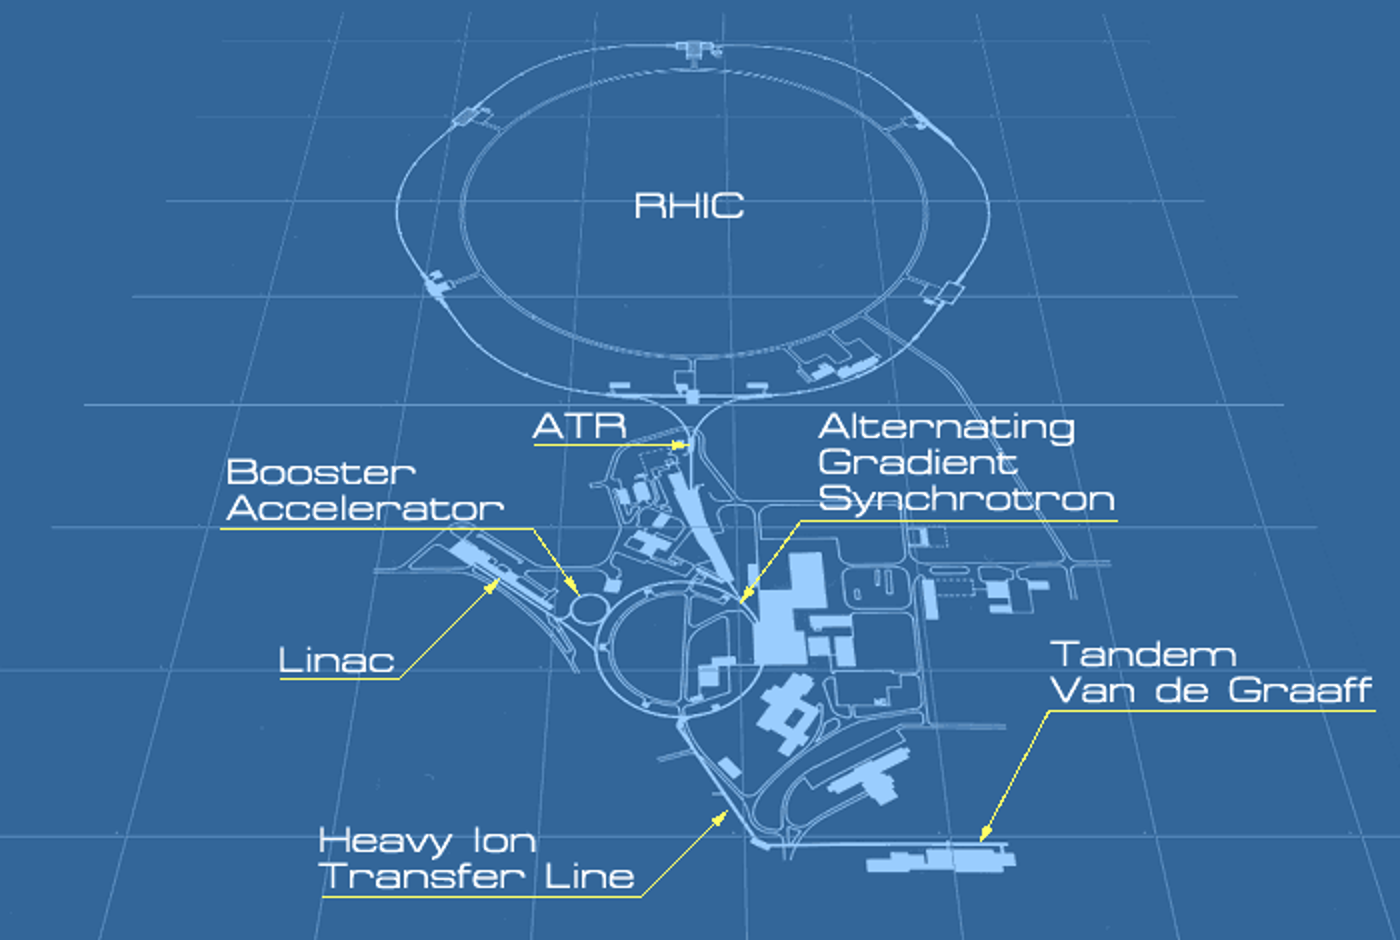
\includegraphics[width=0.8\textwidth]{./figures/RHIC.png}
\caption{位于BNL的相对论重离子对撞机RHIC的加速器示意图。}
\label{Fig:RHIC}
\end{figure}


%\renewcommand{\thechapter}{\arabic{chapter}} % change the chapter counter to be 1
%\thispagestyle{fancy}
位于美国布鲁克海文国家实验室(Brookhaven National Laboratory,简称:BNL)的相对论重离子对撞机(The Relativistic Heavy-Ion Collider, 简称:RHIC)\cite{harrison2003rhic}是世界上第一个专用的重离子对撞机,建立与2000年,从2001年开始为科学家提供了满能量的电子束流~\cite{qgp}。
RHIC是世界上第一个运行的重离子对撞机\cite{harrison2003rhic}。

图\ref{Fig:RHIC}是它的结构示意图。在RHIC装置上,重离子被注入对撞机之前是通过范德格拉夫串列静电加速器(Tandem Van De Graaff),增强器(The Booster Synchrotron),交变梯度同步加速器(Alternating Gradient Synchrotron, 简称:AGS)预加速的~\cite{qgp,harrison2003rhic}。
为了加速一束金原子核,我们先通过脉冲溅射离子源得到带负电的金离子,然后利用第一级的范德格拉夫串列静电加速器进行加速;在这里部分核外电子被位于内部高压终端的箔片剥离;随后带正电的金离子通过第二级装置加速到每核子1. MeV~\cite{harrison2003rhic, qgp}。这些带正电的离子通过传输线到达带有射频电场的增强器中~\cite{qgp}。在增强器中金离子被分为三束团并加速到每核子78MeV,增强器出口的箔片会把所有核外电子剥离,从而我们得到了干净的金原子核,然后金原子核将被注入到AGS之中,AGS会把三束金离子加速到10.8 GeV并注入RHIC环中~\cite{qgp,harrison2003rhic}。RHIC环有两个,分别被称为“蓝(Blue)”环(顺时针方向)和"黄(Yellow)"环(逆时针方向),它们的周长为3.834$Km$,离子在两条环中具有相反的运动方向~\cite{qgp,harrison2003rhic}。RHIC环的束流是建设在同一个水平面上的两个非圆形同心超导磁铁环,两个环在六个不同的位置相互交叉~\cite{qgp,harrison2003rhic},也就是说RHIC环上有6个对撞点,但其中只有4个对撞点装上了探测器,分别为BRAHMS(在2点钟方向);STAR(6点钟方向);PHENIX(8点钟方向);以及PHOBOS(10点钟方向)。目前只有STAR实验装置还在运行中,PHENIX正在升级中。

至今RHIC上进行了一系列的不同碰撞系统、碰撞的能量,其中包括p+p, p+Al, p+Au, d+Au, $\mathrm{He^3}$+Au, Cu+Cu, Cu+Au, Au+Au, U+U, Ru+Ru, Zr+Zr对撞,以及一些低能的固定靶实验(Au+Au)。

\bigskip

\section{STAR探测器}

RHIC上的螺线管径迹探测器(The Solenoidal Tracker At RHIC,简称:STAR)主要是用于研究了解重离子碰撞的时空演化过程,以及碰撞产生的“小爆炸“中所产生的QGP的性质。STAR探测器是由很多的子探测器组成\cite{ackermann2003star}。%主要包括磁铁\cite{bergsma2003star},磁铁是为了提供沿圆筒轴向方向上的均匀磁场;
\begin{figure}[htbp]
\centering
\includegraphics[width=\textwidth,clip]{figure/STAR_detector.png}
\caption{STAR探测器示意图。}
\label{fig:star_overview}
\end{figure}
 每个子探测器都有其特定功能,例如TPC可用于跟踪,在较低的横向动量范围内测量带电粒子的动量,TOF可以识别在较高的横向动量范围内的带电粒子以及VPD可以测量初级碰撞顶点的位置, 适用于重离子碰撞中的逐事件特征。
 图\ref {fig:star_overview}是STAR检测器的示意图。零度量能器(Zero Degree Calorimeters,简称:ZDC)\cite{adler2001rhic}主要是用于探测未参与碰撞的重子的位置信息,可用于重建一阶事件平面;束流计数器(Beam Beam Counters,简称:BBC)\cite{whitten2008beam}主要用统计前向快度区的粒子数,可以通过它的反应作为事件触发的条件和束流质量的检测。时间投影室(Time Projection Chamber,简称:TPC)\cite{anderson2003star},它是STAR的主要的径迹探测器,它提供了带电粒子的碰撞点,用以重建带电粒子的运动径迹,并通过测量电子在磁场中的曲率从而得到粒子的动量并通过电离能损来鉴别粒子,关于TPC的具体功能将在下面进行展开介绍;飞行时间探测器(Time of Flight, 简称:TOF)\cite{bonner2003single,llope2004tofp,llope2005large},它用于测量带电粒子从碰撞顶点飞到探测器的时间,然后加上TPC中提供的信息从而可以计算粒子的静止质量,即可以用于做粒子鉴别,且其效果非常好;
顶点位置探测器(upgraded Pseudo Vertex Position Detectors 简称:upVPD)\cite{llope2014star},它位于束流方向距离对撞点约5.7m的两端,主要是测量束流方向对撞点的位置信息,可以为TOF提供对撞点的起始时间,还可以通过碰撞点的位置对碰撞事件进行初步筛选。
以下将对本文分析中所用到的主要探测器进行介绍。




\subsection{时间投影室}

\begin{figure}[htbp]
\centering
\includegraphics[width=0.8\textwidth]{./figure/STAR_TPC.png}
\caption[TPC探测器 ]{STAR TPC探测器示意图 \cite{anderson2003star}}
\label{Fig:STAR_TPC}
\end{figure}
时间投影室(Time Projection Chamber,简称TPC)~\cite{anderson2003star}是STAR最主要的径迹探测器,主要用来记录带电粒子的运动轨迹及其动量。
TPC综合来电场、磁场并且包含了敏感气体的粒子探测器,它可以提供粒子的三维坐标信息。
通过TPC提供的带电粒子运动轨迹的信息,可以重建事件的碰撞顶点、测量离子的横动量信息,而且可以通过电离能量损失(ionization energy loss,\dEdx)对带电粒子进行鉴别。
 图.\ref{Fig:STAR_TPC}给出的是TPC探测器的示意图。它的赝快度(pseudo-rapidity, 通常用$\eta$表示)接收范围为 $-1 < \eta <1$,而且它具有全方位角的接受度($0<\phi<2\pi$)。TPC主要由两部分组成,一部分是气体漂移室(Drift Chamber),另外一部分是多丝正比室(Multi-Wire Proportional Chamber,简称:MWPC)。如图~\ref{Fig:STAR_TPC2}所示气体漂移室是与束流同轴的圆筒,在圆筒两侧是多丝正比室。
TPC的长度为4.2m,内径为0.5m,外径为2m。当外部磁场提供的磁场强度为0.5T时,TPC所能测量的动量范围为是$0.10 <p_{T}<30$~GeV/c。

\begin{figure}[htbp]
\centering
\includegraphics[width=0.8\textwidth]{./figure/STAR_TPC2.png}
\caption{TPC读出扇形示意图 \cite{anderson2003star}}
\label{Fig:STAR_TPC2}
\end{figure}


在STAR实验中,对撞产生了大量的带电粒子,TPC处在均匀磁场之中因此这些带电粒子的运动轨迹为螺旋形,且该螺旋形在$x-y$平面内的投影是一个圆圈。STAR的读出系统是基于多丝正比室\cite{anderson2003star},TPC的两端分别有12个扇形,如图如图~\ref{Fig:STAR_TPC2}所示每个扇区分为内层和外层。外层扇区有32行读出片,读出片的面积为6.2mm $\times$ 19.5mm,总计3942个,内层扇区有13行读出片,读出片的面积为2.85mm $\times$ 11.5mm, 总计1750 个。外层读出片面积较大,间距较小,能够提供好的粒子能损测量。内层读出片面积小,间距大,位置分辨率较高。每个读出片的位置是固定的,所以它能提供X 和Y 的坐标信息。在Z轴方向,将电子从中心膜到多丝正比室漂移事件分为512个时间段,每个约为100ns。多丝正比室的读出系统能够满足相对论重离子碰撞高频率高粒子数产生的事件采集,金金碰撞中,其读出频率为2KHz。
当带电粒子在漂移室中运动时,每隔一段距离就会与气室中的气体发生相互作用而电离出电子,粒子的漂移速度在130V/cm的均匀电场下的速度约为5.45cm/$\mu$s ,漂移的电子被在TPC的两端的读出系统收集后转换成电信号,然后传送到STAR的数据采集系统,因为读出板只有45层(在后期升级中总共有55层,目前分析的数据都是45层),因此在TPC探测器中运动的粒子在读出板上最多有45 个击中点(即nHitMax最大为45),也就是总共最多可以提供45个位置信息用来拟合带电粒子的径迹。在后期的数据重建的过程中,利用卡尔曼滤波的方法对TPC所采集的碰撞信息对带电粒子径迹进行拟合、计算该径迹的电离能量损失(\dEdx )。
粒子的平均电离能损($\langle dE/dx \rangle$) 由Bethe-Bloch经验公式给出:
\begin{equation}
\label{eq:bethe_bloch}
-\frac{dE}{dX} = 4\pi N_{A}r_{e}^{2}m_{e}c^{2}z^{2}\frac{Z}{A}\frac{1}{\beta^{2}}\big[\frac{1}{2}ln\frac{2m_{e}c^{2}\beta^{2}\gamma^{2}}{I^{2}} - \beta^{2} - \frac{\delta}{2} \big]
\end{equation}
其中,$N_{A}$是阿伏加德罗常数,$I$是所穿越物质的平均激发能,$z$是入射粒子的电荷量,$A$是核子数,$m_{e}$是电子质量,$r_{e}$是电子的经典半径,$\delta$为密度效应修正参数,$\beta$为粒子的速度,$Z$是所穿越物质的原子序数,$\beta = v/c$,$\gamma = 1/\sqrt{1-\beta^{2}}$。
\begin{figure}[htbp]
\centering
\includegraphics[width=0.8\textwidth,clip]{figure/dEdx_39GeV.png}
\caption{带电粒子的电离能损分布图}
\label{fig:tpc_dedx}
\end{figure}
实验中我们通过将粒子的电离能损与该粒子的理论值做比较,以得到他们的标准偏差$n\sigma$,以此来衡量该粒子是否为某个粒子的一个标准:
\begin{equation}
n\sigma = \frac{1}{R} \frac{\langle dE/dx|_{measure} \rangle}{\langle dE/dx|_{theory} \rangle}
\label{eq:nsigma}
\end{equation}
式中的$R$是电离能损分辨率。$n\sigma$越小则证明该粒子的确定性越高。图~\ref{fig:tpc_dedx}是TPC中带电粒子的电离能损随动量的分布图,图中的虚线表示不同粒子的理论计算值随动量的关系。在一定程度上TPC探测器有良好的粒子的鉴别功能,在一些区域则没有表现处很好的鉴别能力,特别是在动量比较大的时候。这就需要加上TOF的信息以提高粒子鉴别的准确度。


\subsection{飞行时间探测器}

\begin{figure}[htbp]
\centering
\includegraphics[width=0.67\textwidth,clip]{figure/STAR_TOF_tray.png}
\caption{STAR飞行时间探测器上的多气隙电阻板室的结构示意图\cite{llope2005large}}
\label{fig:tof_mrpc_view}
\end{figure}

STAR飞行时间探测器(Time of Filght,简称TOF)\cite{llope2005large},它主要用来测量粒子的飞行时间,提高STAR探测器的粒子鉴别能力。它位于TPC的外侧,由120个条形板组成\cite{llope2005large}(TPC的东西两侧各60个)。每个条形板包含34个沿束流方向放置的多气隙电阻板室(Multi-gap Resistive Plate Chamber ,简称:MRPC) 模块\cite{llope2005large}。其赝快度覆盖范围是$|\eta|<1$,方位角是全空间接收的($2\pi$)。
每个TOF的条形板由32个MRPC模块组成。图.\ref{fig:tof_mrpc_view}给出的是STAR飞行时间探测器上的多气隙电阻板室的结构示意图。
MRPC由上下两层读出电极和中间的多层平行玻璃电阻板组成\cite{llope2005large}。玻璃与玻璃之间由尼龙丝隔开,形成均匀的6个气隙。外层玻璃板通过石墨电极加入高压,这样每个气隙之间就充满来均匀的强电场。当带电粒子穿过MRPC时,在气隙中电离的电子会立刻引起雪崩。因为玻璃板是半绝缘的,因此不会对信号造成干扰,那么读出电极上的感应信号就是各个气隙中雪崩的总和。
因为TOF与碰撞顶点的距离$L$是已知的,因此带电粒子的速度($\beta$)和质量($m$)为:
\begin{align}
\beta &= \frac{v}{c}=\frac{L}{c\Delta t}\\
m^{2}&=p^{2}(\frac{1}{\beta}-1)
\end{align}
这里的 $\beta = p/E $ ,$E = \sqrt{p^{2} + m^{2}}$,  $p$是粒子在TPC所测量的动量,$\Delta t$ 是TOF测量的开始时间和VPD测量的停止时间的差值。
\begin{figure}[htbp]
\centering
\includegraphics[width=0.6\textwidth,clip]{figure/mass2_39GeV.png}
\caption{STAR-TOF测量的粒子质量与动量的关系}
\label{fig:tof_beta}
\end{figure}

图.\ref{fig:tof_beta}是在 {\sNN} = 39 GeV下测量的粒子质量与动量的关系。从图中可以清楚的看到不同粒子所属不同颜色的带子是相互分离的,即利用TOF和TPC所提供的信息能够很好的把粒子鉴别清楚。强大的粒子鉴别能力无疑为我们研究QGP的演化过程和性质提供了强大的武器。



\subsection{重味探测器(Heavy Flavor Tracker)}
2014-2016年在RHIC运行的数据采集期间,STAR实验中加入重味探测器(Heavy Flavor Tracker,简称:HFT)。如图~\ref{fig:hftPixel}所示,可以看到它是由三个硅子探测器组成,包括在最外面的一层条形硅探测器(Silicon Strip Detector,简称SSD )~\cite{ARNOLD2003652};在中间一层的硅径迹探测器( Intermediate Silicon Tracker,简称:IST);以及最里的两层像素探测器(PIXEL)\cite{HLTPIXEL,CONTIN201860}。在这三个子探测器的共同作用下对方位角的覆盖范围是$2\pi$。
\begin{figure}[htbp]
\centering
\includegraphics[width=0.67\textwidth,clip]{Figures_Use/HFT.png}
\caption{重味探测器概述图~\cite{Hao_2014}}
\label{fig:hftPixel}
\end{figure}
根据HFT探测器的信息,由于其出色的分辨率,在重建事件碰撞初级顶点的时候起到了很大的作用。在只有TPC和VPD的情况下,筛选好事件的一个重要标准是其重建的碰撞顶点在束流方向的距离不大于30cm。但通过HFT探测器所提供的信息,我们可以更加精确的重建事件的碰撞顶点,此时我们选的好事件的评判标准是重建的碰撞顶点在束流方向的距离不大于6cm。加入HFT的优势显而易见。在我们下面的分析中用到了run16的Au + Au 200 GeV 的数据,采集过程中安装了HFT,因此在此对其做一个简单介绍。



 \cleardoublepage 

\setcounter{section}{0}

\setcounter{figure}{0}
\setcounter{table}{0}
\setcounter{equation}{0}
%==========================================



\chapter{实验上寻找CME信号的方法}

\bigskip

在实验上致力于在重离子碰撞中寻找CME已经持续了十多年年,但目前还没有令人信服的证据表面观测到CME存在的信号。其主要原因碰撞中产生的一些物理背景同样会造成类似的电荷分离效应。这些年大部分理论和实验工作都致力于消除或减少背景带来的贡献。

本章中首先将对目前实验上所用到的基本的观测方法($\gamma$关联方法、R关联方法),及其所遇到的问题进行回顾;接下来对新提出的电荷平衡函数法的有效性进行检验;最后对这三种方法进行了系统的推导以阐明它们之间的联系,并对它们之间的联系进行了检验。


\section{寻找CME的观测方法及现状}

寻找手征磁效应最基本的是要寻找重离子碰撞中沿着磁场方向上的电荷分离,也就是垂直于反应平面方向上的电荷分离。CME的信号大小由公式.~\ref{eq:Fourier_expansion} 中的$a_{1,\pm}$ 来表征,它是方位角分布通过傅立叶展开的第一阶正弦函数的系数,其大小表现的是该事件正负电荷随反应平面的不对称性,也就是垂直于反应平面的分离效应。因为对撞实验中存在不同的净手征性系统,并且他们的概率是相等的,也就是说对所有事件求平均的话$a_{1,\pm}=0$,所有实验上不能通过测量$a_{1,\pm}$ 的大小来寻找CME,而只能通过测量$a_{1,\pm}$的起伏。
目前实验上主要有两种方法:由Sergei A. Voloshin在2004提出来的三粒子$\gamma$ 关联法~\cite{Voloshin:2008dg},该方法是最早提出以及目前应用最广的方法;由Roy A. Lacey和Niseem Magdy提出来的R关联法($R_{{\rm \Psi}_m}(\Delta S)$)~\cite{RCorr-2011,RCorr-2018} 。
以下将对目前这两种方法及其现状进行简要介绍。

\subsection{ $\gamma$ 关联方法的简介及研究现状}

 $\gamma$关联方法~\cite{Voloshin:2008dg}是基于测量由CME所引起的带电粒子之间的方位角关联而设计的,可以简单的用下式表示:
\begin{eqnarray}
\gamma_{112} &\equiv&  \langle \cos(\phi_\alpha + \phi_\beta -2{\rm \Psi_{RP}}) \rangle \nonumber 
\end{eqnarray}
\noindent 从公式中可以看出该方法主要是计算流反应平面与粒子对$\alpha$ 和 $\beta$ 之间关联。而正如前面所提到的,CME所导致的结果是正负电荷的分离。那么正负电子对所对应的$\gamma_{112}$的结果必然会是不同的(详细介绍见\ref{sec.gamma})。在CME信号的作用下异号粒子对$\gamma_{112}^{OS}>0$,而同号电荷对对$\gamma_{112}^{SS}<0$,这是最基本的$\gamma$关联方法对CME的反应结果。
 $\gamma$关联方法在RHIC~\cite{STAR1,Isobarauaustar,STAR3,STAR4,STAR5,TRIBEDY2017740,JieZhao} 和LHC~\cite{ALICE,CMS1,CMS2} 实验上得到了广泛的应用。
 
 图~\ref{fig:gamma112}中给出了$\gamma_112$在RHIC实验中Au+Au对撞下不同质心能量(200,  62.4, 39, 27, 19.6, 11.5和7.7GeV)和LHC实验中Pb+Pb质心能量为2.76TeV下的二阶参与者平面的中心度依赖结果~\cite{Review3}。在STAR实验结果中质心能量为200GeV(图中(b))时,$\gamma_{112}^{OS}$和$\gamma_{112}^{SS}$都随着中心度的增大而减小,造成这个现象的原因可能是被粒子多重数对信号的稀释效果(越中心粒子多重数越多);还有一个可能的原因是偏心碰撞中由于旁观的质子数较多,因其运动产生的磁场就越强,从而导致CME在偏心碰撞中的效果越大。该数据结果很可能是由于CME所造成的。图~\ref{fig:gamma112}中(a)给出的是在LHC实验中Pb+Pb对撞2.76GeV的结果。它的结果与STAR的200GeV的结果的趋势及其相似,其结果也表现出了CME存在的可能性。 STAR实验数据中其他能量的结果与200GeV的类似的趋势,7.7GeV的结果除外。 在7.7GeV中, $\gamma_{112}^{OS}$和$\gamma_{112}^{SS}$在误差棒范围内是相等的,并没有表现出明显的不同,也就是说在这个能量下没有观察到CME的信号。可能是因为在低能对撞中主要是强子相互作用占主要贡献。这些结果都与理论预期相符,似乎我们以及观测到了CME寻找的信号。
 
\begin{figure}[htb]
\begin{center}
\includegraphics[width=\textwidth,clip]{./Figures_Use/CME_STAR_8E_8panel.pdf}
\end{center}
\caption[$\gamma_112$关联方法在RHIC和LHC实验中Au+Au和Pb+Pb系统的分析结果]{$\gamma_112$关联方法在RHIC和LHC实验中Au+Au和Pb+Pb系统的分析结果,图片取自文献~\cite{Review3}}
\label{fig:gamma112}
\end{figure}

\subsubsection{重离子碰撞中背景的影响}

然而随着更深入的研究发现横动量守恒(Global Momentum Conservation, GMC)、局部电荷守恒(Local Charge Conservation, LCC)以及共振态粒子的$v_{2}$的贡献同样会造成假的CME信号~\cite{Review2}。如图~\ref{fig:background},左图是只有CME信号存在下的结果,此时异号($OS$)与同号($SS$)结果的符号不同但大小相当;当加入横动量守恒时(中间的图),会导致同号、异号的结果都压低,此时它们随着坐标轴对称这一现象被打破了;而当同时加入了横动量守恒和LCC效应时,同号和异号又与纯信号时的趋势是类似的。很难认为以上实验结果是单纯的因为CME而导致的。

\begin{figure}[htb]
\begin{center}
\includegraphics[width=\textwidth,clip]{./Figures_Use/cartoon_bkgd.png}
\end{center}
\caption{$\gamma$关联方法中CME信号、横动量守恒和局部电荷守恒的结果,图片取自文献~\cite{Review3}}
\label{fig:background}
\end{figure}

除了GMC和LCC之外,非流关联共振态粒子的衰变同样会造成假的CME。如图\ref{fig:rhobackground},当$\rho$ 衰变成$\pi^{+}$、$\pi^{-}$电子对时,会引入非流的假的CME信号。
\begin{figure}[htb]
\begin{center}
\includegraphics[width=0.65\textwidth,clip]{./Figures_Use/cartoon_rho.png}
\end{center}
\caption{$\rho$ 共振态衰变示意图,图片取自文献~\cite{Review3}}
\label{fig:rhobackground}
\end{figure}

图\ref{fig:Blass}给出了基于Blast-wave理论对背景的研究与STAR实验的对比结果。在该理论模拟中都加入了GMC。红色的点表示的是在化学冻结阶段加入了与实验中相当的LCC的结果;蓝色的点表示的是加入了完美的LCC的结果;黑色的点表示STAR实验的结果。最直观的结果就是在加入了GMC和LCC之后,模拟的结果在只有背景的情况下与STAR实验结果基本重合了。
\begin{figure}[htb]
\begin{center}
\includegraphics[width=\textwidth,clip]{./Figures_Use/pratt.pdf}
\end{center}
\caption{基于Blast-wave理论对LCC和$v2$背景的结果,图片取自文献~~\cite{Review3}}
\label{fig:Blass}
\end{figure}

虽然说实验的结果似乎观查到了CME存在的证据,但因为背景也会造成同样但结果。因此目前还不能下定论说已经观测到的就是CME的信号。
近几年理论和实验上都在致力于扣除或者压低背景在$\gamma$关联方法中的贡献,在此基础上衍生了很多新的观测量(例如: $\gamma_123$, $\kappa_{112} $)。但如何完美的扣除背景带来的效果目前还没有令人信服的解决方法,更多的科研工作还在进行中。



\subsection{ R关联方法的简介及研究现状}

$\gamma$ 关联方法由于背景的影响,无法准确的下定论,Roy A. Lacey和Niseem Magdy提出了一个新的寻找CME的方法——R关联方法($R_{{\rm \Psi}_m}(\Delta S)$)~\cite{RCorr-2011,RCorr-2018}, 其主要原理也是对逐事件的正负粒子方位角之间的起伏来寻找CME的。该方法的定义如下:

\begin{eqnarray}
R_{\Psi_m}(\Delta S) &=& C_{\Psi_m}(\Delta S)/C_{\Psi_m}^{\perp}(\Delta S),  \, m=2,3,  \nonumber \\
C_{\Psi_{m}}(\Delta S) &=&\frac{N_{\text{real}}(\Delta S)}{N_{\text{Shuffled}}(\Delta S)},  \nonumber \\
\Delta S &=& \frac{{\sum\limits_1^p {\sin (\frac{m}{2}\Delta {\varphi_{m} })} }}{p} - 
\frac{{\sum\limits_1^n {\sin (\frac{m}{2}\Delta {\varphi_{m}  })} }}{n},  \nonumber 
\end{eqnarray}

\begin{figure}[htb]
\begin{center}
\includegraphics[width=\textwidth,clip]{./Figures_Use/RcorrNiseem.png}
\end{center}
\caption[R关联方法在AMPT和AVFD中的结果]{R关联方法在AMPT和AVFD中的结果,图片取自文献~\cite{RCorr-2018}}
\label{fig:RcorrNiseem}
\end{figure}

\noindent 其中 $\Delta\phi_m = \phi - \Psi_m$,而$\Delta S$表示的是逐事件的方位角波动, $N_+$($N_-$) 是在该事件中的正(负)电子的数量,$\Delta S$,测量的是事件中正负电子的电偶极矩的差异性,加权平均是用来消除由于探测器不同方位接收度的影响。 通过打乱原始事件中电荷的符号随机打乱(Shuffling),以消除CME信号的所带来的关联,并保证打乱前后正负电荷的数量与原始事件一致,从而计算$N_{\text{Shuffled}}(\Delta S)$,那么这个打乱的事件就没有了CME信号的影响,因而用$N_{\text{real}}(\Delta S)$除以$N_{\text{Shuffled}}(\Delta S)$,将会达到扣除背景的效果~\cite{RCorr-2011,RCorr-2018}。最终以与CME相关的$C_{\Psi_m}(\Delta S)$除以$C_{\Psi_m}^{\perp}(\Delta S)$而得到最终的观测量$R_{\Psi_m}(\Delta S)$。
他们得到的R关联方法在AMPT和AVFD中的模拟结果如图~\ref{fig:RcorrNiseem}所示。$R_{\Psi_2}(\Delta S)$在没有信号的时候是凸起来的、低于1的形状;在AVFD模型中有信号的时候是大于1、凹陷的,且随着CME信号的增大凹陷的程度会增大。而由于三阶反应平面磁场的方向是没有关系的。因此通过三阶反应平面计算的$R_{\Psi_3}(\Delta S)$是与CME信号无关的背景项,因此可以与二阶的信号的一个对比。在他们的模型结果中三阶是向下的、凸起来的。通过这两篇文章~\cite{RCorr-2011,RCorr-2018}中所给出的结果显示R关联方法不仅对信号的反应很灵敏,而且该方法对背景的反应是不同的。即它可以很好的区分背景与信号,是一个非常理想的观测量。并且其实验数据分析的结果显示观测到了CME信号。

\begin{figure}[htb]
\begin{center}
\includegraphics[width=\textwidth,clip]{./Figures_Use/RcorrCopare.pdf}
\end{center}
\caption{R关联方法寻找CME的文章汇总}
\label{tab:RcorrCopare}
\end{figure}

R关联方法也存在一些问题。如图~\ref{tab:RcorrCopare}所示,不同的科研小组运用R关联方法所计算得到的$R_{\Psi_2}(\Delta S)$对背景的反应是不一致的。那么造成不同研究小组之间分析结果不同的原因究竟是什么呢?是运用模型的不同导致的其它原因所导致呢?目前没有明确的定论。R关联方法也需要更深入的研究才能确定是否观测到了CME存在的信号。





\bigskip

\section{寻找CME的新方法:电荷平衡函数法}

最近文献~\cite{Tang2019}中提出了一种利用电荷平衡函数构建的新方法:电荷平衡函数法(Signed Balance Function)。该方法通过电荷平衡函数对碰撞中磁场所引起的横动量方向的波动来寻找CME。以下将对方法的原理进行介绍。

\begin{figure}[htbp]
\centering
\makebox[1cm]{\includegraphics[width=0.37 \textwidth]{./Figures_Use/ChargeSeparation_IsotropicEmission-crop.pdf}}
\caption{一个各向同性事件中粒子在CME作用下的效果图。红色的实线表示正粒子,灰色的虚线表示负粒子。图片来源于:~\citep{Tang2019}}
\label{fig:Aihong_KatongChargeSeparation}
\end{figure}

那么我们究竟要怎样才能找到CME呢?首先让我们来理解一下

CME所带来的效果究竟是怎么样的:对于受磁场$-\hat{B}$作用而形成的正、负粒子对而言,在磁场的作用下会使正、负电子受到磁场作用,从而导致正负电子分别在相反方向上有额外的运动,即横动量分量在磁场方向上得到了增大。也就是说在CME会使得正负电子对的横动量在磁场方向是那个有额外的加强,这是CME所引起的其中一个效应。前面提到的两种CME分析方法主要是基于CME引起的粒子间的方位角关联,它们没有考虑磁场作用对横动量影响。那么让我们重新回到重离子碰撞中时间的方位角分布公式.\ref {eq:Fourier_expansion}:正、负粒子沿着$B$在相反方向上发散,类似于在平行于反应平面方向上的$v_1$。这样就可以通过类似流的特性来表征CME,并且可以利用大量、现有的流相关的复杂的知识来对CME进行研究。但这样方法是有一定局限性的。举个例子,如果一个各向同性事件中粒子在CME作用下,如图图.~\ref{fig:Aihong_KatongChargeSeparation} 所示。可以看到在CME作用下带正电的粒子的横动量向上增大,而于此同时带负电的粒子的横动量向下增大。如果只考虑方位角之间的关联,那么对这个事件的判断就会出错,从而给出错误的判断——这个事件中没有CME。虽然这个问题可以通过对粒子横动量加额外对限制来鉴别,但它不像直接通过磁场作用导致的横动量变化来得直观。电荷平衡函数法就是基于检验由磁场作用而导致的粒子对在磁场方向上的横动量的增量而提出来的新方法。


\subsection{电荷平衡函数法}

平衡函数(Balance Function)的一般形式是用来描述了相空间中的粒子的绝对分离情况~\cite{Bass:2000az,Adams:2003kg}。
在RHIC 和 LHC实验数据分析中,平衡函数在赝快度空间下描述两个平衡粒子之间的赝快度的绝对差异:$\Delta \eta = |\eta_a - \eta_b|$,通常用来研究对撞实验中强子化的衰变~\cite{bf1,bf2,bf3,bf4,bf5}。
电荷平衡函数法( signed balance function),它考虑的是相空间下粒子之间平衡函数的符号,而不是前面所提到的绝对差异。在此之前电荷平衡函数法也被用来研究重离子碰撞中的磁场~\cite{Ye:2018jwq}。在进行具体的介绍之前,先对坐标系统做以下规定:$x$坐标表示的是碰撞参数的方向,也就是反应平面的方向;$y$坐标表示的是垂直于反应平面的方向,也就是磁场所在的方向;$z$坐标则是电子束流的方向。

\begin{figure}[htbp]
\centering
\makebox[1cm]{\includegraphics[width=0.6 \textwidth]{./Figures_Use/BF_cartoon_noy-crop.pdf}}
\caption{SBF方法原理示意图 ~\cite{Tang2019} }
\label{fig:BF_cartoon}
\end{figure}

电荷平衡函数法可以分为以下四步理解:

\textbf{1) 统计粒子对在横动量方向上排序的标记 } 首先考虑横动量在$y$ 方向上的投影 ($p_y$),对于任意的两个粒子$\alpha$ 和 $\beta$。如果$p^\alpha_y >  p^\beta_y$,那么就认为$\alpha$ 粒子是领先于$\beta$粒子的,反之则是跟随。以下两个平衡函数关系式可以很好的描述粒子对之间的这一关系:
\begin{eqnarray}
\begin{aligned}
B_{P} (S) =  \frac{N_{+-}(S)-N_{++}(S)}{N_+},
\end{aligned}
\label{eq:Bp}
\end{eqnarray}
和
\begin{eqnarray}
\begin{aligned}
B_{N} (S) =  \frac{N_{-+}(S)-N_{--}(S)}{N_-}.
\end{aligned}
\label{eq:Bn}
\end{eqnarray}
这里的下标$P$ 和 $N$ 分别表示正、负粒子项。
对于给定的项$N_{\alpha\beta}$,若$\alpha$ 领先于 $\beta$ 那么标记$S=+1$,反之 $S=-1$ 。$N_{+(-)}$表示的是在一个事件中正、负粒子的个数。


\textbf{2) 计算净的横动量排序的区别 } 一个事件中正、负粒子领先的标记的不同可以表示为:
\begin{eqnarray}
\begin{aligned}
\delta B(\pm 1) =  B_{P}(\pm 1)-B_{N}(\pm 1),
\end{aligned}
\label{eq:deltaB_pm}
\end{eqnarray}

\begin{figure}[htbp]
\centering
\makebox[1cm]{\includegraphics[width=0.45 \textwidth]{./Figures_Use/BFHisto_lab_example.pdf}}
\caption{Toy模型中不同CME情况下$\Delta B$ 的分布图 ~\cite{Tang2019} }
\label{fig:BFHisto_lab_example}
\end{figure}
那么,在这个事件中正、负粒子总标记的不同可以由正粒子领先标记减去负离子跟随的标记,即有:
\begin{eqnarray}
\begin{aligned}
\Delta B =  \delta B(+1) - \delta B(-1).
\end{aligned}
\label{eq:deltaB}
\end{eqnarray}

$\Delta B$ 是表示一个事件总的净横动量排序的不同。在没有CME的情况下,对于正、负粒子对,正粒子领先于负粒子的概率与它跟随的概率是相等的。也就是说此时$B_P$和$B_N$所测的是粒子间与分离效应无关的关联,即都是背景,它的分布只依赖于统计起伏( 图.~\ref{fig:BF_cartoon}上面的图)。 在CME的影响下,因为正负电荷分离效应的存在,其结果是其中一种粒子领先于另一种粒子。在此的情况下$B_P$和$B_N$不再相等,最终结果就是$\Delta B$的宽度会增大( 如图.~\ref{fig:BF_cartoon}下半部分所示)

因为$\Delta B$ 计算的是在每个事件中在一个方向上的起伏。

$\Delta B$ 可以分别从 $x$的方向 ($\Delta B_{x}$) 和 $y$ 方向 ($\Delta B_{y}$)方向计算。但由于在$x$方向上没有磁场的作用——没有CME,$\Delta B_{x}$分布的宽度与CME信号无关。图.~\ref{fig:BFHisto_lab_example} 中描述的是$\Delta B_{x}$ 和 $\Delta B_{y}$ 在Toy 模型中得到的结果。可以明显看得当在原始粒子(Primordial particles)中加入一定量的CME信号($a_1$)时,$\Delta B_y$的宽度要比$\Delta B_x$的要大。


\textbf{3) 计算逐事件的净横动量在$y$方向上的增强} 为了减去统计起伏和背景的影响,可以对不同方向上的$\Delta B$做商,即有:
\begin{eqnarray}
\begin{aligned}
r= \sigma_{\Delta B_y} / \sigma_{\Delta B_{x}}.
\end{aligned}
\label{eq:r}
\end{eqnarray}

那么况下$r=1$ ,有信号时在信号的作用下将大于1。也就是有CME信号时:$r > 1$。

\begin{figure}[htbp]
\centering
\makebox[1cm]{\includegraphics[width=0.76 \textwidth]{./Figures_Use/boost_cartoon-crop.pdf}}
\caption{不同参考系下观察一对粒子的领先与跟随效应原理图~\cite{Tang2019}}
\label{fig:boost_cartoon}
\end{figure}

\textbf{4) 比较从不同参考系下得到的结果 } 我们的观测量$r$ 既可以在实验室坐标系下计算,即$r_{\mathrm{lab}}$ ;也可以在粒子对的静止坐标系下得到$r_{\mathrm{rest}}$。在电荷平衡函数方法中需要要判断粒子对在横动量方向上的跟随情况。如图.~\ref{fig:boost_cartoon} 所描述的是具有相同$p_y$的粒子在不同参考系下的视图,如果在静止坐标系下观察两个粒子的横动量在$y$方向上的排序关系时,很难分清这两个粒子的关系;但如果在这个粒子对的静止坐标系下,而在静止坐标系下两个粒子永远时背对背运动的,那么一目了然的就能知道粒子$\alpha$ 领先于$\beta$。这个特性会让电荷平衡函数的领先、跟随情况更加清楚、准确,因此对于该方法而言静止坐标系时观测CME的最佳坐标。这里我们把静止坐标系下计算将可以得到$r_{\mathrm{rest}}$。

 图.~\ref{fig:BFHisto_rest_lab_example} 是在实验室系、粒子对坐标系下得到的加入了CME信号的Toy模型中$\Delta B_x$ 和 $\Delta B_y$ 的分布结果,其中放大的部分是分布的峰顶的区域。当我们看$y$方向上的$\Delta B_y$的分布时,静止坐标系下的分布宽度要比实验室系下要宽;然而在$x$方向上却没有观察到这一现象。这也就是说在有CME的时候,静止坐标系下能够更明显的观测到CME的效果。
\begin{figure}[htbp]
\centering
\makebox[1cm]{\includegraphics[width=0.56 \textwidth]{./Figures_Use/BFHisto_rest_lab_2pcta1_example.pdf}}
\caption{Toy模型中在不同坐标系下$\Delta B_x$ 和 $\Delta B_y$的分布结果~\cite{Tang2019}}
\label{fig:BFHisto_rest_lab_example}
\end{figure}


考虑到在$r$下并不能保证完全扣除背景的影响,而静止坐标系下能够更好的观测CME信号。那么将不同坐标系的结果相除,以此进一步扣除$r$中残存的背景贡献,则有:
\begin{eqnarray}
\begin{aligned}
R_{B} \equiv  \frac{r_{\mathrm{rest}}}{r_{\mathrm{lab}}},
\end{aligned}
\label{eq:R_B}
\end{eqnarray}
这里的“$B$”表示的是平衡函数(Balance function)。在接下来的多种模型的分析结果中,会得到这样一个现象:当$r_{\mathrm{rest}}$,$r_{\mathrm{lab}}$和$R_{B}$随信号的增大而增大时,而于此同时$R_{B}$会随着背景(共振态$v_2$、全局的自旋极化等背景)增大而减小。在某些情况下,这个性质对于识别由于背景引起的电荷分离效应是非常有用的。例如,如果$r_{\mathrm{rest}} $大于1, 并且$R_{B}$也大于1,那么就有理由相信这个情况下有CME的效果存在。


\subsection{模型计算结果分析、更新与总结}

前面已经提到在寻找CME的过程中最大的问题是背景也会对观测量有一定的贡献,在本小节中,我们将利用最简单的Toy模型(既可以加入信号也可以加入背景),AMPT模型(包含实验数据中的各种背景)以及EBE-AVFD模型(包括了很多实验数据中的的背景,也可以加入信号),该小节的内容可以在这篇文章中找到~\cite{Lin2021}。
\begin{figure}[htbp]
\centering
\makebox[1cm]{\includegraphics[width=0.56 \textwidth]{./finalplots/fig2.pdf}}
\caption{Toy模型中加入CME信号、共振态$v_2$时\rrest, $r_{\mathrm{lab}}$和\rb 的结果~\cite{Lin2021}。}
\label{fig:resonancev2}
\end{figure} 

\subsubsection{Toy模型}
因为在Toy模型中,我们可以任意的加入我们需要的信号($a_{1}$ )以及各种背景,例如:共振态的$v_2$,$\rho_{00}$自旋极化所引起的背景等。首先让我们看看在只有信号的情况下,如图.~\ref{fig:ToySignalOnly}所示,图中以原初粒子的$a_1$为横坐标,其中$a_1$就是前面所提到的CME的信号。从图中可以看到,当$a_1$为0时,$r_{\mathrm{rest}}$, $r_{\mathrm{lab}}$和 $R_{\mathrm{B}}$都等于1,而随着$a_1$的增大三个观测量也都随之而增大。$r_{\mathrm{rest}}$和 $r_{\mathrm{lab}}$的结果很接近,但是可以明显看到在有信号的情况下$r_{\mathrm{rest}}$比$r_{\mathrm{lab}}$要大,前者比后者对信号对反应更灵敏,这一结果也可以在$R_{\mathrm{B}}$表现出来。这一结果表明SBF方法中对观测量对信号是很敏感的。考虑到$r_{\mathrm{rest}}$和 $r_{\mathrm{lab}}$的性质相近而$r_{\mathrm{rest}}$对信号的反应更加灵敏,所以在接下来的讨论中我们将只这对$r_{\mathrm{rest}}$和$R_{\mathrm{B}}$进行分析。

共振态$v_2$对SBF观测量的影响在图.~\ref{fig:resonancev2}中给出。从图中可以看到\rb 随着共振态$v_2$的增大而减小,而此时\rrest 是随之而增大的。这两个观测量在各种不同的横动量谱下的共振态的影响下表现出相反的趋势。关于SBF方法在Toy模型在各种不同情况下的反映可以在这篇引文~\cite{Tang2020}中看到更加详细的研究。

\begin{figure}[htbp]
\centering
\makebox[1cm]{\includegraphics[width=0.56 \textwidth]{./finalplots/fig3.pdf}}
\caption{Toy模型中加入CME信号、共振态$v_2$和$\rho_{00}$之后\rrest 和\rb 的结果~\cite{Lin2021}。}
\label{fig:resonancerho00}
\end{figure} 

在图.~\ref{fig:resonancerho00}中,加入了CME研究中主要的两个背景:共振态$v_2$和共振态的全局极化$\rho_{00}$( Global Spin alignment ),这是在Toy模型中加入背景最多、最接近实验的情况。从图中可以清楚的看到在背景逐渐增大的时候,\rrest 和\rb 出现了相反的趋势,即在\rrest 随着信号、背景而增大的时候\rb 反而在减小,并且在背景增大到一定程度上的时候\rb 小于1。那么也就是说,在不考虑局部电荷守恒(Local Charge Conservation,简称:LCC)和横动量守恒(Transverse Momentum Conservation,简称:TMC)的前提下,如果\rrest 和\rb 都大于1的话,那么我们可以认为我们观测到了CME信号。


\subsubsection{AMPT与EBE-AVFD模型}

前面通过Toy模型的检测我们基本可以确认SBF方法是可以鉴别信号和背景的,那么在更接近实际实验中的AMPT模型和EBE-AVFD模型中我们的方法是否依然有效呢?接下来我们将对此展开讨论。首先允许我再对两个模型进行简要介绍。我们所用的两个模型都是目前比较热门的模型,它们对实验数据中一些主要的特征(粒子谱,椭圆流等)都描述得很好,在一定程度上能够反应实验数据的特性。
本工作中所用的AMPT模型是还在改进的版本,在这一版本中没有CME的信号加入,但模型中包含了TMC对粒子的影响。因此AMPT的结果将作为没有CME信号下,即纯背景对于观测量的结果,它可以作为无信号情况下的参考。
EBE-AVFD模型中加入了可以调节CME信号的机制,其CME信号通过轴向电荷与熵的比值表征(\ns ),此外它还控制加入的LCC的效应的大小。利用EBE-AVFD模型我们可以进行定量的、系统的对信号、背景对观测量的反应进行研究。
图.~\ref{fig:realisticmodel}给出的就是这两个模型下的随重心度依赖的结果(对于EBE-AVFD模型只给出了一个中心度:$30-40\%$)。
\begin{figure}[htbp]
\centering
\makebox[1cm]{\includegraphics[width=0.56 \textwidth]{./finalplots/fig4.pdf}}
\caption{\rrest 和\rb 在AMPT和AVFD模型中的结果。}
\label{fig:realisticmodel}
\end{figure} 
为了与STAR实验组的接收度相统一,本分析中用到的截断是$|\eta|<1$ 和 $0.2 < p_{T} < 2$ \gevc ,即与实验数据分析中所用到的截断一致。从图中可以看到,对于没有CME信号的两种情况:AMPT和AVFD\ns =0的情况下,$r_{\mathrm{rest}}$ 与 $R_{\mathrm{B}}$ 在统计误差范围内都为1。而在有EBE-AVFD中有CME的情况下不论LCC =  33\% 或者 LCC = 0\%,两个观测量都随着\ns 的增大而增大。在CME的效果下两个观测量都有明显的增大。对比不同大小的LCC情况下,可以看到实心的LCC为0的时候要比空心的LCC = 33\% 时要稍大,更详细的关于LCC影响的工作还在进行。但我要说明的是LCC = 33\% 是根据STAR实验采集的Au + Au 200 \gev 的计算得到的。也就是说LCC = 33\% 是更接近实验事实的,而此时的结果我们能够清楚的看得CME的信号。在后面~\ref{AuAuresults}与实验结果的对比中LCC = 33\% 。


%本章将由以下几个部分构成:在第一部分,我们将对三种实验上用于寻找手征磁效应方法:$\gamma$ 关联($\gamma$ correlator)~\cite{Voloshin:2008dg}, $R$关联和电荷平衡函数(Signed Balance Functions)~\cite{Tang2019,Lin2021},对他们之间的相关性进行研究讨论。第二部分,我们将利用简单的蒙特卡洛模拟和以及包括流等其他效应的Event-By-Event Anomalous-Viscous Fluid Dynamics (EBE-AVFD)~\cite{Shi:2017cpu,Jiang:2016wve,Shi:2019wzi},对寻找守征磁效应对方法进行比较研究。
%第四部分将利用AVFD模型所产生的Isobar的数据,系统的比较三种方法在相同信号、背景下对CME信号的灵敏度进行分析比较。
%最后一部分将对本章做对工作和结果做一个总结。

\bigskip

\section{实验观测方法之间的相关性}
\label{Sec.II}
本章节将对以上所提到的三种基本方法:$\gamma$关联方法~\cite{Voloshin:2008dg}, R关联方法 ($R_{{\rm \Psi}_m}(\Delta S)$)~\cite{RCorr-2011,RCorr-2018} 和电荷平衡函数法~\cite{Tang2019,Lin2021}。这些方法所利用的最基本的信息都是碰撞中所产生磁场对粒子在磁场方向上的关联,因而不同方法都包含了相同的信息。这部分将对这三种方法进行回顾,并揭示他们之间的联系。


\subsection{$\gamma$ 关联法}
\label{sec.gamma}

三粒子关联方法 $\gamma$ (在后面对介绍中主要指 $\gamma_{112}$) 所测量的是相对于反应平面的电荷分离或者$a_{1,\pm}$ 系数的波动~\cite{Voloshin:2008dg},
\begin{eqnarray}
\gamma_{112} &\equiv&  \langle \cos(\phi_\alpha + \phi_\beta -2{\rm \Psi_{RP}}) \rangle \nonumber \\
&=& \langle\cos(\Delta\phi_{\alpha})\cos(\Delta\phi_{\beta}) -
\sin(\Delta\phi_{\alpha})\sin(\Delta\phi_{\beta})\rangle \nonumber \\
&=& (\langle v_{1,\alpha}v_{1,\beta}\rangle + B_{\rm IN}) -(\langle a_{1,\alpha}a_{1,\beta}\rangle + B_{\rm OUT}), \label{eq:ThreePoint}
\end{eqnarray}
\noindent 上式中取平均分两部分,首先是对一个事件中$\alpha$ 和 $\beta$ 所能组成的粒子对进行平均,然后再对所有的事件取平均。
对三角函数进行展开,可以明显的看到方位角关联在垂直于反应平面( {\it in-plane} )和平行于反应平面({\it out-of-plane} )他们之间的不同。在公式~\ref{eq:ThreePoint}中第三项 $\langle a_{1,\alpha}a_{1,\beta}\rangle$,所表示对就是$a_{1,\pm}$ 系数的波动,这也就是我们寻找CME的主要目标。其它项是与CME无关的:其中$\langle v_{1,\alpha}v_{1,\beta}\rangle$ 是与直接流相关的,并且该项在对称的核核对撞中是与电荷的符号、电磁场无关的;$B_{\rm IN}$ 和 $B_{\rm OUT}$ 这两项分别表示的是垂直与平行反应平面的其它可能存在的背景所带来的贡献。如果我们考虑异号电荷(Opposite-sign,简称:OS)和同号电荷(Same-sign,简称:SS)的 $\gamma_{112}$ 的不同时有:
\begin{equation}
\Delta \gamma_{112} \equiv \gamma^{\rm OS}_{112} - \gamma^{\rm SS}_{112}, 
\end{equation}
\noindent 通过异号与同号做差,直接流相关贡献除去了;其中还残留的背景贡献是与流平面相关的$B_{\rm IN}-B_{\rm OUT}$项,它的大小与椭圆流成正相关性,这是$\Delta \gamma_{112}$ 观测量中主要的背景来源。在实际运用中,流平面可以近似的用实验中探测到的末态粒子重建的事件平面(Event plane,简称:EP),另外由于有效的事件平面分辨率影响,观测量需要对此进行修正~\cite{Poskanzer:1998yz}。
$\gamma_{112}$ 方法主要对优势在于它直接与$a_1$ 相联系,而且只需要一个简单对过程对事件平面进行修正。

 $\Delta\gamma_{112}$观测方法中与流相关对背景研究可以共振态衰变为例子。如果共振态通过QGP介质运动,那它们的衰变后产生的粒子将会在垂直于流平面对方向上造成电荷分离的效应~\cite{fuqiang2010,Schlichting:2010qia}。运动的共振态会导致局部或者整个事件的横动量守恒(Transverse momentum conservation,简称:TMC)~\cite{Pratt:2010zn,Bzdak:2012ia} 或者局部电荷守恒(Local charge conservation,简称:LCC)~\cite{Schlichting:2010qia}。理想情况下的二粒子关联可以写为:
\begin{eqnarray}
\delta &\equiv& \langle \cos(\phi_\alpha -\phi_\beta) \rangle \nonumber \\
&=& (\langle v_{1,\alpha}v_{1,\beta}\rangle + B_{\rm IN}) +(\langle a_{1,\alpha}a_{1,\beta}\rangle + B_{\rm OUT}),
\label{eq:delta}
\end{eqnarray}
它同样包含了CME对信号$\langle a_{1,\alpha} a_{1,\beta} \rangle$对贡献,但事实上二粒子关联中占主要贡献对是短程对而粒子关联。
例如,在$\Delta \delta$ 和 $\Delta \gamma_{112}$中,TMC效应的贡献可以用一下关系式表示\cite{Bzdak:2012ia}:
\begin{eqnarray}
\Delta \delta^{\rm TMC} &\rightarrow& -\frac{1}{N}
\frac{\langle p_T \rangle^2_{\rm \Omega}}{\langle p_T^2 \rangle_{\rm F}}
\frac{1+({\bar v}_{2,{\rm \Omega}})^2-2{\bar{\bar v}}_{2,{\rm F}}{\bar v}_{2,{\rm \Omega}}} {1-({\bar{\bar v}}_{2,{\rm F}})^2},
\label{eq:TMC1}
\\
\Delta \gamma^{\rm TMC}_{112} &\rightarrow& -\frac{1}{N}
\frac{\langle p_T \rangle^2_{\rm \Omega}}{\langle p_T^2 \rangle_{\rm F}}
\frac{2{\bar v}_{2,{\rm \Omega}}-{\bar{\bar v}}_{2,{\rm F}}-{\bar{\bar v}}_{2,{\rm F}}({\bar v}_{2,{\rm \Omega}})^2} {1-({\bar{\bar v}}_{2,{\rm F}})^2}
\nonumber \\
&\approx& \kappa^{\rm TMC}_{112} \cdot v_{2,{\rm \Omega}} \cdot \Delta \delta^{\rm TMC},
\label{eq:TMC2}
\end{eqnarray}
其中 $\kappa^{\rm TMC}_{112} = (2{\bar v}_{2,{\rm \Omega}}-{\bar{\bar v}}_{2,{\rm F}})/v_{2,{\rm \Omega}}$, ${\bar v}_{2}$ 和 ${\bar{\bar v}}_{2}$ 分别表示$v_2$对于 $p_T$- 和 $p_T^2$-的权重。下标“F”表示在全空间下对所有产生对粒子取平均,然而实际上在实验中能够探测到的只是所有产生的粒子中的一小部分,所有用“${\rm \Omega}$”表示实际能够测量到的这一部分。LCC所带来的贡献与公式~\ref{eq:TMC1} 和公式 ~\ref{eq:TMC2}有相同的结构特点~\cite{Pratt:2010zn,Schlichting:2010qia}。
基于此我们可以利用$v_2$ 和 $\Delta \delta$对$\Delta \gamma$ 进行归一化:
%This motivates a normalization of $\Delta \gamma$ by $v_2$ and $\Delta \delta$:
\begin{equation}
    \kappa_{112} \equiv \frac{\Delta \gamma_{112}}{v_2 \cdot \Delta \delta}.
\label{kappa112}
\end{equation}
 只有当$\kappa_{112}$大于 $\kappa^{\rm TMC/LCC}_{112}$的情况下才有可能说找到了CME。在现在$\kappa^{\rm TMC/LCC}_{112}$ 的影响还没有可靠的估算的情况下,只有通过Isobar两个碰撞系统的$\Delta\gamma_{112}$(和$\kappa_{112}$)的结果比较才能对是否有CME信号给出更加明确的结论。 
%While a reliable estimate of $\kappa^{\rm TMC/LCC}_{112}$ is still elusive, the comparison of $\Delta\gamma_{112}$ (and $\kappa_{112}$) between isobaric collisions may give a more definite conclusion on the CME signal.

\subsubsection{其他的衍生的 $\gamma$ 关联法}
在以上介绍的$\gamma$ (以及对应的$\kappa$)关联方法的基础上,为了更好的估算 $\kappa_{112}$中背景的贡献~\cite{CMS2},例如:
\begin{eqnarray}
\gamma_{123} \equiv \langle \langle \cos(\phi_\alpha + 2\phi_\beta -3{\rm \Psi_{3}}) \rangle\rangle&,~\ & \kappa_{123} \equiv \frac{\Delta \gamma_{123}}{v_3 \cdot \Delta \delta}, 
\\
\gamma_{132} \equiv \langle \langle \cos(\phi_\alpha - 3\phi_\beta + 2{\rm \Psi_{2}}) \rangle\rangle&,~\ &
\kappa_{132} \equiv \frac{\Delta \gamma_{132}}{v_2 \cdot \Delta \delta}.
\end{eqnarray}
其中 $\Psi_{2}$ 和$\Psi_{3}$ 分别表示 二阶($2^{\rm nd}$- order)和 三阶($3^{\rm rd}$-order)反应平面。
式中$\Delta\gamma_{123}$ 和$\Delta\gamma_{132}$ 两项对应的贡献主要是$(v_3 \cdot \Delta\delta)$ 和 $(v_2 \cdot \Delta\delta)$,他们对信号没有反应。因此,在一定程度上可以认为这两个项所反应的结果是完全的背景。然而由于在只有信号的模型AMPT的AuAu碰撞数据的计算结果表明$\kappa_{123}$ 和 $\kappa_{132}$ 与$\kappa_{112}$不相等,这与预期有一定的出入~\cite{Subikash}。因此在接下来的方法比较中,我们将不对这些衍生的$\gamma$ 方法进行研究。

\subsubsection{MSC 和 CMAC}
在 $\gamma_{112}$ 关联方法中,电荷分离的不同的方位角区间所做的权重是不一样的。在与反应平面成$90^\circ$ 角,也就是垂直与反应平面的粒子对的权重要比与反应平面的夹角较小的哪些粒子对的权重要大。为了解决这个问题,MSC~\cite{STAR3} 的方法尝试对$\gamma_{112}$进行改进,以便所有电荷分离的不同方位角方向上都取同样的权重。
详细的说也就是说如果粒子对中两个粒子的夹角在$90^\circ$ 的粒子的权重,在此基础上公式.~\ref{eq:ThreePoint} 改写为:
\begin{equation}
\langle \cos(\phi_{\alpha}+\phi_{\beta}-2{\rm \Psi_{RP}}) \rangle =
\langle (M_{\alpha}M_{\beta}S_{\alpha}S_{\beta})_{\rm IN} \rangle -
\langle (M_{\alpha}M_{\beta}S_{\alpha}S_{\beta})_{\rm OUT} \rangle,
\label{eq:MMSS}    
\end{equation}
其中$M$ 表示所有的幅度(Absolute magnitude )($0\leq M \leq 1$) ,  $S$ 表示$\sin$或$\cos$项的符号($\pm 1$)。$IN$和$OUT$分别表示公式~\ref{eq:ThreePoint} 中的$\cos$项和$\cos$项。在忽略$\gamma_{112}$中$M$的贡献的前提下,得到:
\begin{equation}
{\rm MSC} \equiv \left(\frac{\pi}{4}\right)^2\left({\langle S_{\alpha}S_{\beta} \rangle_{\rm IN}-\langle S_{\alpha}S_{\beta}\rangle_{\rm OUT}}\right).
\label{eq:msc}    
\end{equation}
在AuAu 200 GeV的结果中, MSC方法基本得到了与$\gamma_{112}$关联方法同样的趋势,只是大小一些微小的差别~\cite{STAR3}。
同样的,MSC方法同样可以通过计算相对于反应平面的电荷来实现。对于同号电荷对在垂直于反应平面的关联可以表示为:
\begin{equation}
\langle S_{\alpha}S_{\beta}\rangle_{\rm IN} =
\frac{N_{\delta}^{\rm L}\left(N_{\delta}^{\rm L}-1\right) + N_{\delta}^{\rm R}\left(N_{\delta}^{\rm R}-1\right) -
  2N_{\delta}^{\rm L}N_{\delta}^{\rm R}}{N_{\delta}\left(N_{\delta}-1\right)},
\label{eq:NetCombosSS}  
\end{equation}
其中,当$\alpha\beta=++$时$\delta=+$。当$\alpha\beta=--$时,$\delta=-$ 。
同理的异号电荷对可以表示为:
\begin{equation}
\langle S_{\alpha}S_{\beta}\rangle_{\rm IN} =
\frac{N_{+}^{\rm L}N_{-}^{\rm L} + N_{+}^{\rm R}N_{-}^{\rm R} -
  N_{+}^{\rm L}N_{-}^{\rm R} - N_{-}^{\rm L}N_{+}^{\rm R}}{N_{+}N_{-}}.
\label{eq:NetCombosOS}
\end{equation}
上式中$N$ 表示对是检测到到粒子是正还是负、是横动量空间下粒子是在垂直于反应平面的左边($L$)或者右边$R$。同理的平行于反应平面的结果也可以用相同结果的式子,只需要把左、右改成上、下。


另外还有一个类似的计算电荷的方法叫做CMAC~\cite{STAR4},它也得到了类似于MSC方法得到的结果。MSC和CMAC方法与 $\gamma_{112}$原理上是大致相当的,只是这两个方法与$a_1$ 不是直接相关的,并且他们对于事件平面分辨率没有直接的修正方法。因此在本文中不会用这两种方法。但在这两个方法的基础上我们可以把$\gamma_{112}$ 关联方法与其他的方法联系起来,因此对这两个方法做了简要介绍。

\subsection{$R$ 关联法}
%The $R(\Delta S_m)$ correlator~\cite{RCorr-2011,RCorr-2018} takes the double ratio of four event-by-event distributions,
$R(\Delta S_m)$ 关联方法\cite{RCorr-2011,RCorr-2018} 是通过对四个逐事件分布的的比值来寻找CME的信号的,即:
\begin{equation}
R(\Delta S_m) \equiv \frac{N(\Delta S_{m,\rm real})}{N(\Delta S_{m,\rm shuffled})} / \frac{N(\Delta S^{\perp}_{m,\rm real})}{N(\Delta S^{\perp}_{m,\rm shuffled})}, ~\ m = 2,3,...,
\end{equation}
式中一个事件中垂直于$m^{\rm th}$阶反应平面($\Psi_m$)的电荷分离可以写作:
\begin{equation}
\Delta S_{m,\rm real} = \langle\sin(\frac{m}{2}\Delta\phi_m)\rangle_{N_+} - \langle\sin(\frac{m}{2}\Delta\phi_m)\rangle_{N_-}.   
\end{equation}
这里的 $\Delta\phi_m = \phi - \Psi_m$, $N_+$($N_-$) 是在该事件中的正(负)电子的数量。加权平均可以消除由于探测器不同方位接受度的影响。 把上式中的$\Psi_m$ 替换为$( \Psi_m + \pi/m)$, 则得到 $\Delta S^{\perp}_m$,它表示平行于事件平面的电荷分离,同理有$\Delta S_m$,这两项表征的是与磁场无关的背景项。
$\Delta S^{(\perp)}_{m,\rm shuffled}$ 项是通过对一个事件中对正负电荷随机打乱(Shuffling),但保证打乱前后正负电荷的数量与原始事件一致,然后对打乱后的事件进行计算得到。在理想情况下,CME会令$R(\Delta S_2)$ 的分布呈现凹(Concave shape)下去的形状,它与$R(\Delta S_3)$的形状是不一样的~\cite{RCorr-2018}。据推测,后者与 $\gamma_{123}$具有相同的效果,都是用来表示没有CME信号的对比作用。

通过对$R(\Delta S_2)$的分布进行高斯(或反高斯,需根据具体形状选择)函数进行拟合,而所得到的高斯分布的宽度(Gaussian width,$\sigma_{R2}$ )将用作最终的反应CME信号的观测量。由于$\Delta S^{(\perp)}_{2,\rm real(shuffled)}$这四个项都基本上符合高斯分布,我们可以得到$\sigma_{R2}$ 和这四个项的方差(RMS)的值的关系:
\begin{equation}
\frac{S_{\rm concavity}}{\sigma_{R2}^2}   = \frac{1}{\langle (\Delta S_{2,\rm real})^2 \rangle} - \frac{1}{\langle (\Delta S_{2,\rm shuffled})^2\rangle} - \frac{1}{\langle (\Delta S_{2,\rm real}^{\perp})^2  \rangle} + \frac{1}{\langle (\Delta S_{2,\rm shuffled}^{\perp})^2  \rangle}.
\label{eq:sigma_R2} 
\end{equation}
其中$S_{\rm concavity}$的符号由$R(\Delta S_2)$的形状决定,如果它是凸起的是$+1$,反之则为$-1$。首先让我们先理解一下上式中右边各项的意义。为了简便,我们将以1为权重,则等式右边第一项可以展开为:
\begin{eqnarray}
& &(\Delta S_{2,\rm real})^2 \nonumber \\
&\equiv& (\frac{\sum_{i=1}^{N_+}\sin(\Delta\phi_i)}{N_+}-\frac{\sum_{i=1}^{N_-}\sin(\Delta\phi_i)}{N_-})^2 \nonumber \\
&=& \frac{\sum_{i=1}^{N_+}\sin^2(\Delta\phi_i)+\sum_{i\neq j}^{N_+}\sin(\Delta\phi_i)\sin(\Delta\phi_j)}{N_+^2}+\frac{\sum_{i=1}^{N_-}\sin^2(\Delta\phi_i)+\sum_{i\neq j}^{N_-}\sin(\Delta\phi_i)\sin(\Delta\phi_j)}{N_-^2}\nonumber \\
& &-\frac{2\sum_{i=1,j=1}^{N_+,N_-}\sin(\Delta\phi_i)\sin(\Delta\phi_j)}{N_+N_-} \nonumber \\
&=& \frac{\langle \sin^2(\Delta\phi_i)\rangle_{N_+} +(N_+-1) \langle \sin(\Delta\phi_i)\sin(\Delta\phi_j)\rangle_{N_+N_+}}{N_+}  \nonumber \\
 && +\frac{\langle \sin^2(\Delta\phi_i)\rangle_{N_-} +(N_--1) \langle \sin(\Delta\phi_i)\sin(\Delta\phi_j)\rangle_{N_-N_-}}{N_-} \nonumber \\
& &-2\langle \sin(\Delta\phi_i)\sin(\Delta\phi_j) \rangle_{N_+N_-}
\label{eq:dS}
\end{eqnarray}
利用三角恒等式, $\sin^2(x) = [1-\cos(2x)]/2$ 和 $2\sin(x)\sin(y) = \cos(x-y)-\cos(x+y)$,我们将得到公式~\ref{eq:dS} 对所有事件对均值:
\begin{eqnarray}
\langle(\Delta S_{2,\rm real})^2\rangle 
&=& \frac{1-v_2^+}{2N_+} + \frac{N_+-1}{2N_+}(\delta^{++}-\gamma^{++}_{112})+\frac{1-v_2^-}{2N_-}  \nonumber \\
&&+ \frac{N_--1}{2N_-}(\delta^{--}-\gamma^{--}_{112}) - (\delta^{+-}-\gamma^{+-}_{112}) \\
&\approx& \frac{2(1-v_2-\delta^{\rm SS}+\gamma_{112}^{\rm SS})}{M} - \Delta\delta + \Delta\gamma_{112}.
\label{eq:s-expand}
\end{eqnarray}
最后一行我们假设:$v_2^+ \approx v_2^-$, $N_+ \approx N_- = M/2$。即使在假设的近似估算之前我们也可以看到$\langle(\Delta S_{2,\rm real})^2\rangle$ 项可以用$N_{+(-)}$, $v_2$, $\delta$ 和 $\gamma_{112}$替换,可以得到:
\begin{eqnarray}
\langle(\Delta S_{2,\rm real}^\perp)^2\rangle 
&=& \frac{1+v_2^+}{2N_+} + \frac{N_+-1}{2N_+}(\delta^{++}+\gamma^{++}_{112})  \nonumber \\
 && +\frac{1+v_2^-}{2N_-} + \frac{N_--1}{2N_-}(\delta^{--}+\gamma^{--}_{112}) - (\delta^{+-}+\gamma^{+-}_{112}) \\
&\approx& \frac{2(1+v_2-\delta^{\rm SS}-\gamma_{112}^{\rm SS})}{M} - \Delta\delta - \Delta\gamma_{112}.
\label{eq:sp-expand}
\end{eqnarray}
对于shuffled项,$v_2^+$ 和$v_2^-$可以用$(v_2^+ + v_2^-)/2$替换,那么$\delta$则可以用$(\delta^{\rm OS}+\delta^{\rm SS})/2$替换。并且整个$\gamma$关联方法可以用 $(\gamma^{\rm OS}+\gamma^{\rm SS})/2$替换。因此我们得到:
\begin{eqnarray}
\langle(\Delta S_{2,\rm shuffled})^2\rangle 
&\approx& \frac{2(1-v_2)-\delta^{\rm SS}-\delta^{\rm OS}+\gamma_{112}^{\rm SS}+\gamma_{112}^{\rm OS}}{M}
\label{eq:s-S-expand}\\
\langle(\Delta S_{2,\rm shuffled}^\perp)^2\rangle 
&\approx& \frac{2(1+v_2)-\delta^{\rm SS}-\delta^{\rm OS}-\gamma_{112}^{\rm SS}-\gamma_{112}^{\rm OS}}{M}.
\label{eq:sp-S-expand}
\end{eqnarray}
因此,在基于$R(\Delta S_2)$的四个组成部分之间的双重消除之下,我们构造了一个与 $\Delta\gamma_{112}$相联系的关系式:
\begin{eqnarray}
\Delta_{R2} & \equiv &\langle (\Delta S_{2,\rm real})^2 \rangle - \langle (\Delta S_{2,\rm shuffled})^2 \rangle - \langle (\Delta S^{\perp}_{2,\rm real})^2 \rangle  + \langle (\Delta S^{\perp}_{2,\rm shuffled})^2 \rangle   \nonumber \\
 &\approx &2(1-\frac{1}{M})\Delta \gamma_{112}.
\label{eq:relation1}
\end{eqnarray}
这个关系式将在后面的几个部分中详细测试。为了进一步阐明最终的观测量$\sigma^2_{R2}$ 和$\Delta\gamma$之间的联系,我们将公式~\ref{eq:s-expand}, ~\ref{eq:sp-expand},~\ref{eq:s-S-expand} 和~\ref{eq:sp-S-expand} 代入公式.~\ref{eq:sigma_R2},即可得到:
\begin{equation}
\frac{S_{\rm concavity}}{\sigma_{R2}^2} \approx -\frac{M}{2}(M-1)\Delta\gamma_{112}.    
\label{eq:relation2}
\end{equation}
这里我们假设$\langle (\Delta S_2)^2\rangle$的四个相关项和$\frac{2}{M}$远远大于其它因素的贡献,在一般情况下$\Delta\delta$ 具有最大的影响。

公式.~\ref{eq:relation2} 所表示的关系表明如果$\Delta\gamma$是正的、有限的,那么$R(\Delta S_2)$ 的分布将呈现下凹的形状,反之亦然。反应平面分辨率的修正对于$\Delta_{R2}$ 和 $\sigma^2_{R2}$是很微小的,它的影响可以忽略不计,公式.~\ref{eq:relation1} 、 \ref{eq:relation2}提供了实现这个目标的近似方法。



\subsection{电荷平衡函数方法}

另一个寻找CME的方法就是上一章中提到的SBF方法~\cite{Tang2019},
\begin{eqnarray}
\Delta B_y 
&\equiv& [\frac{N_{y(+-)}-N_{y(++)}}{N_+} - \frac{N_{y(-+)}-N_{y(--)}}{N_-}] - [\frac{N_{y(-+)}-N_{y(++)}}{N_+} - \frac{N_{y(+-)}-N_{y(--)}}{N_-}] \nonumber \\
&=& \frac{N_+ + N_-}{N_+N_-}[N_{y(+-)} - N_{y(-+)}].
\label{eq:by}
\end{eqnarray}
其中 $N_{y(\alpha\beta)}$是一个逐事件的量,它表示在垂直与反应平面方向上粒子对中$\alpha$领先于粒子$\beta$ 的粒子对的个数 ($p_y^\alpha > p_y^\beta$)。
同理的我们可以计算 $\Delta B_x$,表示在平行于反应平面方向上粒子$\alpha$领先于粒子$\beta$ 的粒子对的个数。然后最终的观测量是基于$\Delta B_y$ 和 $\Delta B_x$ 分布的宽度,即
\begin{equation}
r \equiv \sigma(\Delta B_y) / \sigma(\Delta B_x).
\label{rlab}
\end{equation}
由于CME导致的电荷分离效应会使在垂直于反应平面的方向上($y$方向,与磁场方向平行)的粒子对的投影的波动会比另一个方向上要大。
$r$ 可以在实验室坐标系下计算,即有$r_{\rm lab}$,也可以在静止坐标系下计算:$r_{\rm rest}$,且认为在静止坐标系下观察电荷分离效应是最好的。并且他们之间的商:
\begin{equation}
R_B = r_{\rm rest} / r_{\rm lab},
\end{equation}
能够更好的帮助区分背景还是真正的CME信号。
%An extra care is also needed to correct the $r$ observable for the event plane resolution.

在一个事件中,我们对$\Delta B_y$各个项重新解析得到:
\begin{equation}
N_{y(\alpha\beta)}-N_{y(\beta\alpha)} = \sum_{\alpha,\beta} {\rm Sign}[p_{T,\alpha}\sin(\Delta\phi_\alpha)-p_{T,\beta}\sin(\Delta\phi_\beta)].    
\end{equation}
因此,为了与其它方法相关联,假设$p_T$是平均横动量,这样就可以先不考虑横动量的影响。在只考虑方位角的情况下,与其它方法一样展开。直接使用$[\sin(\Delta\phi_\alpha) - \sin(\Delta\phi_\beta)]$对Sign()项进行展开,这里需要引入一个归一化因子$C_y$,那么对事件取平均的结果则有:
\begin{eqnarray}
\langle N_{y(\alpha\beta)}-N_{y(\beta\alpha)} \rangle &\approx& C_y \Big\langle \sum_{\alpha,\beta} [\sin(\Delta\phi_\alpha) - \sin(\Delta\phi_\beta)] \Big\rangle \nonumber \\
&=& C_y \Big\langle [N_\beta \sum_{\alpha}\sin(\Delta\phi_\alpha) - N_\alpha \sum_{\beta}\sin(\Delta\phi_\beta)] \Big\rangle \nonumber \\
&=& C_y N_\alpha N_\beta \langle \langle \sin(\Delta \phi)\rangle _{N_\alpha}-\langle \sin(\Delta\phi)\rangle_{N_\beta} \rangle. \label{eq:constant}
\end{eqnarray}
常数可以通过计算粒子对数计算,再加上式..~\ref{eq:Fourier_expansion}中$\frac{dN}{d\Delta\phi}$ ,则有:
\begin{eqnarray}
\langle N_{y(\alpha\beta)}-N_{y(\beta\alpha)} \rangle &=& 2\int_{-\pi/2}^{\pi/2} 
\Big[\int_{-\pi/2}^{\Delta\phi_\alpha} \frac{dN}{d\Delta\phi_\beta}d\Delta\phi_\beta+\int_{\pi-\Delta\phi_\alpha}^{3\pi/2} \frac{dN}{d\Delta\phi_\beta}d\Delta\phi_\beta   \nonumber \\
&& -\int^{\pi-\Delta\phi_\alpha}_{\Delta\phi_\alpha} \frac{dN}{d\Delta\phi_\beta}d\Delta\phi_\beta\Big]\frac{dN}{d\Delta\phi_\alpha}d\Delta\phi_\alpha \nonumber \\
&\approx& \frac{8}{\pi^2}(1+\frac{2}{3}v_2)N_\alpha N_\beta (a_{1,\alpha}-a_{1,\beta}).  \label{eq:integral_result}  
\end{eqnarray}
通过比较公式.~\ref{eq:constant} 和\ref{eq:integral_result},我们可以得到$C_y = 8(1+2v_2/3)/\pi^2$。在不考虑 $p_T$ 的权重的情况下$\langle\Delta B_y\rangle$ 变成$\frac{8(1+2v_2/3)}{\pi^2} M \langle\langle \sin(\Delta \phi)\rangle_{N_+} -\langle \sin(\Delta\phi)\rangle_{N_-} \rangle$,它的函数形式与$\langle S_{2,\rm real}\rangle$类似。
因此类似的我们假设:
\begin{equation}
\langle N_{x(\alpha\beta)}-N_{x(\beta\alpha)} \rangle \approx  C_x N_\alpha N_\beta \langle\langle \cos(\Delta \phi)\rangle _{N_\alpha}-\langle \cos(\Delta\phi)\rangle_{N_\beta} \rangle,  
\end{equation}
直接的计算统计可以改写为:
\begin{eqnarray}
\langle N_{x(\alpha\beta)}-N_{x(\beta\alpha)} \rangle &=& 2\int_{0}^{\pi} 
\Big[\int_{\Delta\phi_\alpha}^{2\pi-\Delta\phi_\alpha} \frac{dN}{d\Delta\phi_\beta}d\Delta\phi_\beta-\int^{\Delta\phi_\alpha}_{-\Delta\phi_\alpha} \frac{dN}{d\Delta\phi_\beta}d\Delta\phi_\beta\Big]\frac{dN}{d\Delta\phi_\alpha}d\Delta\phi_\alpha \nonumber \\
&\approx& \frac{8}{\pi^2}(1-\frac{2}{3}v_2)N_\alpha N_\beta (v_{1,\alpha}-v_{1,\beta}).   
\end{eqnarray}
因此$C_x = 8(1-2v_2/3)/\pi^2$, 
式$\langle\Delta B_x\rangle$ 替换为 $\frac{8(1-2v_2/3)}{\pi^2} M \langle\langle \cos(\Delta \phi)\rangle_{N_+} -\langle \cos(\Delta\phi)\rangle_{N_-} \rangle$,相似的有 $\langle \Delta S_{2,\rm real}^{\perp}\rangle$. 

现实中 $\langle\Delta B_{y(x)}\rangle$和$\langle \Delta S_{2,\rm real}^{(\perp)}\rangle$ 这两项为0。可见$C_y$ 和$C_x$ 这两项主要包含了SBF方法的影响因素。因为我们的目标是把$\Delta B_y$、$\Delta B_x$分布的方差与其他方法联系起来,在此给出以下两个关系式(详细推导见附录\ref{appendix1}):

\begin{eqnarray}
\sigma^2(\Delta B_y) &\approx& \frac{4M}{3}+ \frac{64M^2}{\pi^4}(1+ \frac{4}{3} v_2)(a_{1,+}-a_{1,-})^2 
\\
\sigma^2(\Delta B_x) &\approx& \frac{4M}{3}+ \frac{64M^2}{\pi^4}(1-\frac{4}{3}v_2)(v_{1,+}-v_{1,-})^2 .
\end{eqnarray}
那么与 $\gamma$关联方法的相关联,可以有:
\begin{equation}
\Delta_{\rm SBF} \equiv \sigma^2(\Delta B_y) - \sigma^2(\Delta B_x) \approx  \frac{128M^2}{\pi^4}(\Delta\gamma_{112}-\frac{4}{3}v_2\Delta\delta).   \label{eq:relation3} 
\end{equation}
需要说明的是因为SBF不仅考虑了粒子的方位角,而且考虑了他们的横动量信息。如果式.~\ref{rlab} 中用$\sigma^2(\Delta B_y) - \sigma^2({\Delta B_x})$替换,那么如果考虑了横动量的权重时它将大致等效于 $(\Delta \gamma_{112}-\frac{4}{3}v_2\Delta\delta)$


\subsection{三种方法核心部分的比较}
\label{Sec:kernel}
这一部分,我们将通过研究Toy模型和EBE-AVFD 以此验证在上一部分介绍的他们之间的关系:$\gamma$ correlator: $\Delta \gamma_{112}$;$R$ correlator, :$\Delta_{R2}$;SBF:$\Delta_{\rm SBF}$
我们的目标是通过验证各个方法对与信号、背景的反应,并确认这些实验方法之间的关系式是否成立(式.~\ref{eq:relation1} 和 \ref{eq:relation3})
为了方便起见,在这一部分中的结果是在反应平面之下计算的。用于分析的粒子的截断为:$|\eta|<1$ , $0.2 < p_T < 2$ GeV/$c$.


\begin{figure}[htbp]
\centering
\includegraphics[width=6.2cm]{./Figures_Use/fig_toy.pdf}
\caption[三种方法核心组成部分在Toy模型中的结果]]{Toy模型中 $2\Delta\gamma_{112}$, $\Delta_{R2}$ 和$\Delta'_{\rm SBF}\equiv(\frac{\pi^4}{64M^2}\Delta_{\rm SBF}+\frac{8}{3}v_2\Delta\delta)$ 的结果}
\label{fig:toya1}
\end{figure}

\subsection{Toy模型}
我们把三种方法的的主要关系式在完全相同的数据、截断下做分析。图\ref{fig:toya1} 给出的是以 $a_1^2$为横坐标,三种不同方法的组成部分:$2\Delta\gamma_{112}$, $\Delta_{R2}$ 和 $\Delta'_{\rm SBF}\equiv(\frac{\pi^4}{64M^2}\Delta_{\rm SBF}+\frac{8}{3}v_2\Delta\delta)$ 的结果。空心的图形表示的是纯信号的情况下,实心的是加入了信号和共振态衰变的情况下的结果,也就是说这两种情况前一种情况是没有背景的而后一种是包括了共振态$v_2$的情况。
在没有背景的情况下,三个观测量的核心组成部分都具有基本相同的结果,并且他们都落在$4a_1^2$的线性函数之上。因此,三种方法都都同样都CME信号有相同都灵敏度。在这种理想的情况下,$\Delta_{\rm SBF}$ 考虑的横动量信息似乎没有明显的区别。
当加入共振态$v_2$的影响的情况下,对于所有三种方法,在纯信号贡献的基础上都表现出了相当大的背景效果。而且这一现象在信号越小的时候表现得更加明显。在Toy模型中加入的共振态背景对三种方法的都有类似的反应。当然其中也纯在着一些细微的差异,可能是在公式~\ref{eq:relation1} 、\ref{eq:relation3}的推导中忽略了高阶项的结果引起的。尽管背景的影响取决于粒子谱的不同,尤其是椭圆流共振态的粒子谱~\cite{Feng:2018chm,Schlichting:2010qia,Pratt:2010zn},但一般而言,我们相信这三种方法在一个大范围大粒子谱和共振态的情形下会有相同的反应。


\subsection{EBE-AVFD模型}
在EBE-AVFD 模型中包含了CME的信号并且该模型中的背景以更加接近与实验中的真实包含的背景。在接下来的模拟之中,我们产生了EBE-AVFD 中心度为30-40\% Au+Au 碰撞在$\sqrt{s_{\rm NN}} = 200$ GeV的事件, 其中 $n_{5}/s$ = 0, 0.1 和 0.2。因此在这三种情况下他们的背景基本是保持不变的,通过改变$n_{5}/s$来改变来CME的信号大小。因为反应平面已知,因此可以得到在模型中的$a_{1,\pm}$的值,见表.\ref{tab:Observeda1AuAu} 。
\begin{center}
\begin{table}[h]
\centering
\caption{ EBE-AVFD模型AuAu对撞200GeV中的值}
\begin{tabular}{c|c|c}
\toprule
 $n_{5}/s$    &  Positive particles      &   Negative particles   \\  
\hline
0   &  0 & 0 \\
0.10 &  0.0082   $\pm$ 0.0001   &  -0.0067 $\pm$ 0.0001  \\
0.20 &  0.0154   $\pm$ 0.0001   &  -0.0146 $\pm$ 0.0001  \\
\bottomrule
\end{tabular}
\label{tab:Observeda1AuAu}
\end{table}
\end{center}



图.~\ref{fig:AVFD_delta}(a) 给出了三个核心组成部分$2\Delta\gamma_{112}$, $\Delta_{R2}$ , $\Delta'_{\rm SBF}$以\ns 为横坐标的结果。这三个方法的结果在相同的\ns 下都有着非常相似的结果,从而进一步证实了式~\ref{eq:relation1} 和 \ref{eq:relation2}所表示的关系的正确性。
\begin{figure}[htbp]
\vspace*{-0.01in}
\centering
\subfigure{\includegraphics[width=6.2cm]{./figures/fig_AVFD.pdf}}
\subfigure{\includegraphics[width=6.2cm]{./figures/fig_Equ42.pdf}}
\captionof{figure}[三种方法核心组成部分在EBE-AVFD中的结果]{三种方法核心组成部分在EBE-AVFD中的结果:(a) 以\ns 为横坐标(以此检验式.~\ref{eq:Superposition};(b) 扣除全背景项之后的结果。} \label{fig:AVFD_delta}
\end{figure}
由于EBE-AVFD模型事件的反应平面是已知的,我们可以很容易的得到$a_{1,\pm}$的值,如表.\ref{tab:Observeda1AuAu}所示,在知道模型数据中$a_1$的情况下我们能够更好的解释不同\ns 的结果。从表中可以看到$a_{1,\pm} = 0$这与$n_{5}/s=0$是一致的,并且$a_{1,+}$和$a_{1,+}$的值在一定的$n_{5}/s$范围内是有限的而且他们之间的符号是相反的。因为在对撞系统中会包含额外的正电荷,因此正、负电荷的$a_{1}$不一定是完全相等的。
根据$\gamma_{112}$ correlator 在式中的的展开项和三种方之间的关联我们期望这三个方法的核心组成部分($O(n_{5}/s)$)都能够服以下公式:
\begin{center}
\begin{equation}
O(n_{5}/s) - O(0) =  a_{1,+}^2 + a_{1,-}^2 - 2a_{1,+}a_{1,-}.
\label{eq:Superposition}
\end{equation}
\end{center}
图.~\ref{fig:AVFD_delta}(b) 所给出的是三种方法在扣除全背景的情形下的结果,三种方法的结果都落在了同一条直线上。EBE-AVFD模型的结果揭示了实验观测量对信号和背景贡献的线性叠加关系。本文中的模型结果证实了大多数尝试将信号和背景分离的分析方法都默认假设了这一点。

在Toy模型和EBE-AVFD模型对三种方法核心组成部分的比较结果表明在一般意义上说三种实验室的观测量对于相同的CME信号、背景的反应是彼此等同的。并没有哪种研究方法比另外的方法更要有优势的说法。
%The kernel-component comparison using both the toy model and the EBE-AVFD model support the idea that to the first order, the three observables are equivalent to each other, with their very similar responses to the CME signal as well as the backgrounds. Up to this point, we see no  obvious advantage of one over the others.  




\section{本章小结与讨论}


本章在第一部分对目前实验上用于寻找CME信号的观测方法:$\gamma$ 关联方法和R关联方法目前的研究现状进行介绍。通过两种方法计算得到的结果都表面实验中有可能观测到了CME信号存在的可能性。但是两种方法都存在仍未解决的问题。背$\gamma$关联方法观测量中信号与背景的贡献很难区分、鉴别,GMC、LCC和共振态衰变所带来的非流关联都可能引起假的CME信号;并且在理论模拟中只包含背景的情况下也可以重现STAR实验在Au+Au对撞200GeV能量下的测量的结果。R关联方法就提出这一方法的作者的结果而言,是一个非常完美的观测量,他们的模型结果表面该方法对信号与背景的是截然不同的,能够轻松的鉴别信号与背景。但它存在的问题是其他人(除了方法提出者之外的人)并不能重复出他们的结果。那么这个不同是什么原因造成的呢?是提出这所用的模型不同还是不同研究者之间程序之间可能存在问题?这个问题需要进一步的验证。因此该方法的结果也不能作为观测到CME信号证据。

在第二部分对新提出的以检验碰撞中磁场所引起的横动量方向的波动来寻找CME的电荷平衡函数法,本文对该方法的模型检验进行来回顾与更新,对该方法的一组观测量对信号、背景的反映进行来进一步的检验。通过对Toy模型中不同信号、背景混合的情况下的研究方检验发现\rrest 和\rb 对CME信号的反应都很灵敏,并且两者对背景有着不同的反应:在\rrest 随着背景的增大而增大时\rb 会随着背景的增大而减小。这一性质无疑让我们能够很好的鉴别信号与背景。最后在更加接近实验数据的AMPT模型和EBE-AVFD模型中的结果也表明我们的方法是能够区分信号与背景的。模型的检验已经证明SBF方法是有效的。下一步就是将该方法应用在实验数据分析中,其分析过程与结果在下一章给出。

在第三部分对三种方法$ \gamma$关联方法、R关联方法和电荷平衡函数法进行了详细详细的推导,最终表面三种方法是相互联系的;
在Toy模型和EBE-AVFD模型对三种方法核心组成部分的比较结果表明三种实验室的观测量对于相同的CME信号、背景的反应是彼此等同的。并没有哪种研究方法比另外的方法更要有优势的说法。
%本章中关于Toy模型与AMPT的模拟主要由导师唐爱红完成,本人只是做了一些更新、检查工作;关于EBE-AVFD模型的结果与STAR数据的分析全部由本人完成。

 \cleardoublepage 

\setcounter{section}{0}

\setcounter{figure}{0}
\setcounter{table}{0}
\setcounter{equation}{0}
%==========================================
\chapter{ 电荷平衡函数法在Au+Au~200~GeV的分析结果与讨论}

在上一章中引入了通过测量CME所引起的在磁场方向的横动量分布的波动来寻找CME信号的新方法—— 电荷平衡函数法,多种模型的结果证明该方法所引出的两个观测量\rrest 和\rb 对CME信号都有很好的反应,而且背景对该方法的两个观测量有着不同的放应。即在CME信号的作用下,\rrest 和\rb 都会大于1;\rrest 会随着背景的增大而增大,而与此同时\rb 会压低,且小于1。因此如果\rrest 和\rb 都大于1那就是CME信号存在到证据。模型的检验结果表面通过对比电荷平衡函数的这一组观测量可以很好的鉴别信号与背景。

RHIC@STAR实验对撞点的数据采集以及持续了二十几年,在此期间采集了不同质心能量($\sqrt{s_{\mathrm{NN}}} =  $ 7.7, 11.5, 14.5, 19.6, 27, 39, 54.4, 62.4 and 200 GeV )的Au+Au对撞、200GeV UU对撞、pPb对撞以及固定靶的数据,如此多的不同能量、对撞系统的数据无疑为研究QGP对性质提供了一个非常好的平台。对与CME的研究而言,如果我们能够证实CME确实存在,更深入的我们可以研究在什么条件下(质心能量、碰撞系统等)发生了破缺,这必然对我们了解、掌握手征奇异性的性质具有重要意义。因为CME是由磁场引起的,而磁场是由旁观质子的运动而产生的,质心能量越大磁场越强,则能观察到信号的几率就越大。电荷平衡函数法是利用了多次做商来消除背景的贡献,因此该方法对统计量的要求比较高,在此我们优先对2016年所采集的Au+Au~200~GeV进行研究分析。

\begin{figure}[htbp]
\centering
\includegraphics[width=14cm,clip]{./Figures_Use/run16BadrunQA.png}
\caption{run16 Au+Au200GeV中run的QA图}
\label{fig:badrun}
\end{figure}

\section{分析数据的记录与筛选}
数据采集过程中会把所有的碰撞信息都记录下来。一般情况下每隔一段时间就会对所采集的事件进行一次存储,且根据当时存储的时间进行记录,在对撞实验组中会以20分钟为一个记录,记住一个run。由于实验的探测器并不是随时都能保持最佳的工作状态,运行过程中有可能会出现一些不能用于分析的run,所以需要对这些存储下来run的质量进行筛选。如图\ref{fig:badrun}是不同run的QA图。由于探测器、束流的影响,不同run的$<|VertexZ-pdVz|>$和不同时期的值是不一样的。图中上线两条现外的run表示是距离这个时期run的标准差太远的,称为不好的run(bad run)。这些run是不会应用与数据分析中的。





\subsection{事件筛选}
并不是所记录的所有事件都是好的事件。为了减少这些额外的背景对分析的影响,在分析过程中会对坏的事件进行筛选。
在本文的分析中所用到的是挑选触发最小偏差(Minimal Bias Trigger, MB) 事件。Minimum Bias trigger 的数据是通过挑选零度量能器(ZDC)两侧的通量和顶点探测器(VPD)探测到的碰撞顶点来挑选。一下是几个最基本的事件筛选的条件:
\begin{figure}[htbp]
\centering
\includegraphics[width=14cm,clip]{./Figures_Use/VpdVz.png}
\caption{AuAu200GeV中对碰撞顶点筛选后的结果}
\label{Fig:VpdVz}
\end{figure}

\begin{itemize}
\item 通过TPC所重建的初级顶点(Primary Vertex)在束流(z)方向上的距离不能太远,取决于不同的能量,即$|V_z| < $常数。
\item 初级顶点在垂直于束流的方向(X-Y)上的投影距离TPC的中心小于2cm,即$Vr < 2 cm$。
\item 在碰撞能量大于等于39GeV(即39,62.4和200GeV)时,VPD重建的顶点位置和TPC重建的初级顶点在z方向上的投影之间的距离要小于3cm,即 $|Vz^{VPD}-Vz^{TPC}| < 3cm$,主要目的是去除在同一事件发生多次碰撞的事件,即碰撞的顶点不只一个(Pile-up event)。
\end{itemize}
STAR合作组在16年采集数据的时候加入了HFT探测器,有了HFT探测器会显著提高事件重建的顶点的位置,因此在本文的分析中采用$|V_z| < 6.0   cm$。(在没有HFT探测器的时候是利用VPD所重建的初级顶点来筛选事件的,精确度比较低,此时要求$|V_z| < 30.0 cm$)。图.~\ref{Fig:VpdVz}是本文分析中菜用的截断之后的结果,因为所用的数据(picoDst)已经预先加入了$|V_{z}^{VPD}-V_{z}^{TPC}| < 3.0$因此左图中只有筛选之后的一条色带。从图中可以看到大部分的事件都是集中在中心位置。
表~\ref{tab:Event_cut}中列出了我们在分析Au+Au200GeV是对事件筛选用到的截断。run16 Au+Au 200GeV在对所有截断之后总共得到将近$1*10^{9}$的好事件。
\begin{table}[htb]
\centering
\caption{Au + Au 200 GeV事件挑选的基本条件}
\begin{tabular}{c|c|c|c|c}
\toprule
$\sqrt{s}_{NN}$  &  $|V_{z}|$(cm)  &  $V_{r}$(cm)  &  $|V_{z}^{VPD}-V_{z}^{TPC}|$  &  Trigger ID (MB)                          \\ \hline
200 run16       &  $<$ 6          &  $<$ 2        &  $<$ 3                        &       5200-01, 11, 21, 31, 41, 51    \\ 
\bottomrule
\end{tabular}
\label{tab:Event_cut}
\end{table}

STAR合作组提供了一个C++的标准类:StRefMultCorr,它同时包含了中心度的划分以及事件对于中心度和亮度(Luminosity)的权重,所有的中心对划分都包括在里面。如果\ref{fig:centrality},根据事件中末态粒子多种数的多少划分中心度(实验中不能直接测量碰撞参数,只能通过末态粒子多重数的大小来区分碰撞的中心度)。在STAR实验组的划分中,末态粒子数小于总事件数$80\%$的部分在分析中是扣除的。从$80\%-0\%$表示的是由偏心碰撞到中心碰撞,即$0\%-5\%$是表示的是事件中末态粒子数最多的那一部分。

\begin{figure}[htbp]
\centering
\includegraphics[width=14cm,clip]{./Figures_Use/run16centrality.png}
\caption{run16 Au+Au200GeV的中心度分布结果}
\label{fig:centrality}
\end{figure}


\subsection{带电粒子径迹的筛选}
从TPC我们会得到很多与粒子径迹相关的信息,为了保证分析中所用到的带电粒子纯度比较高。下面是一些相关参数的简要介绍及用到的截断:
\begin{itemize}
\item $DCA$:带电粒子径迹距离重建的初级碰撞顶点的最近距离,在本文的分析中默认设置是$d_{ca}$ < 1 cm。
\item nFitFits: TPC中拟合带电粒子径迹所用到的碰撞点的个数不得少于15个(总共有45个)。
\item nHitdDdx:带电粒子径迹用于计算电离能量损失的径迹不得少于5个。
\item rnHitsFit/nHitsPoss >0.52: 表示拟合径迹的碰撞点与可能是该径迹的碰撞点的个数的比值不能少于0.52%。以此保证去除可能分裂的径迹。
\end{itemize}
以上是对带电粒子径迹的质量的筛选。因为带电粒子的质量会影响最终观测量的结果,为了计算系统误差,在以上默认设置之外,还会对不同的截断的结果进行分析以估算最终观测量的系统误差。这一点在后面会详细介绍。

\subsection{带电粒子径迹的筛选}
在实验中探测器能探测到的粒子有三种:$\pi$、$K$ 和$p$。而碰撞中产额最高的是$\pi$介子,它占了末态粒子大部分。因此在本文的分析中我们只对$\pi$介子进行分析。也因此我们需要对末态粒子进行鉴别。粒子的鉴别主要用到TPC~\cite{Anderson:2003ur} 和TOF~\cite{Llope:2005yw}。TPC探测器可以提供带电粒子的电离能损、动量信息,通过与粒子的理论值相的比较得到它相对于理论值的偏差($n\sigma$ ),其偏差越小表示它是该种粒子的概率越大。通过TOF可以得到粒子在探测器中的飞行时间,再把粒子的横动量也考虑近去就能够计算出粒子的静止质量($m$),通过对质量做截断会提高粒子对纯度。图.\ref{Fig:PID}左图给出了在筛选之前对TPC中横动量与电离能损对关系图,可以看到由不同色带所表示的不同的粒子种类;右图中是通过TOF和TPC信息测量的质量随横动量的分布图,通过不同的质量平方的分布可以清晰的分辨不同的粒子。
\begin{figure}[htbp]
\centering
\includegraphics[width=14cm,clip]{./Figures_Use/PID.png}
\caption{TPC与TOF的粒子鉴别}
\label{Fig:PID}
\end{figure}
表.~\ref{tab:Track_cut}中列出了在我们的分析工作中具体的动力学和粒子鉴别截断。通过这个截断,我们能够更多的利用探测器检测到的带电粒子信息,从而能够更好的放映真实碰撞的物理过程。
\begin{table}[htb]
\centering
\caption{数据分析中具体的动力学、粒子鉴别所用的截断}
    \centering
   \resizebox{\textwidth}{!}{
\begin{tabular}{|c|c|c|}
\toprule
	\sNN$(GeV)$   & 动力学截断& 粒子鉴别截断 \\ \midrule[0.5pt]
 & \multirow{2}{*}{$|\eta| < 1.0 $ } & {\color{red}TPC}\\ 
	Au+Au    &  & $|n\sigma_{p}|$ < 2 \\ \cline{2-3} 
	200 GeV  &  \multirow{2}{*}{ $0.2 < p_T<2.0 $ (GeV/c)   }  & {\color{red}TPC+TOF} \\
					&   &$|n\sigma_{p}|$ < 3 \quad $-0.01<m^2<0.1 (\mathrm{GeV}/c^{2})^{2}$ \\  %\midrule[0.5pt]
\bottomrule
\end{tabular}
}
\label{tab:Track_cut}
\end{table}




\bigskip
\section{事件平面法}

因为CME是跟磁场方向有关的,而磁场的方向与反应平面(一阶、二阶)是垂直的。因此需要了解事件的反应平面位置。因为实验中是无法直接得到碰撞的反应平面,只能利用实验中探测到的粒子来重建事件平面以此来估计反应平面。由于重建的反应平面是根据接收的粒子进行的重建,其与真实反应平面是有一定的偏差的,事件平面分辨率(Event plane resolusion)是表征事件平面与反应平面的偏差~\cite{Poskanzer:1998yz,Voloshin:2008dg}。

反应平面通过流矢量$Q_{n}$的计算来得到,其定义如下:
\begin{equation}
\label{eq:Qn_x}
Q_{\textbf{n},x} = \sum_{i}\omega_{i}\mathrm{cos}(n\varphi_{i})
\end{equation}
\begin{equation}
\label{eq:Qn_y}
Q_{\textbf{n},y} = \sum_{i}\omega_{i}\mathrm{sin}(n\varphi_{i})
\end{equation}
这里的n表示事件平面的阶数。那么事件平面的与事件流矢量$Q_{n}$之间的关系可以表示为:
\begin{equation}
\label{eq:EventPlane}
\Psi_{n} = \frac{1}{n} \mathrm{arctan}(\frac{Q_{\textbf{n},y}}{Q_{\textbf{n},x}})
\end{equation}
\begin{figure}[htbp]
\centering
\includegraphics[width=0.67\textwidth,clip]{./Figures_Use/fig_EPreconstructed30-40.pdf}
\caption{AuAu200GeV反应平面重建及修正}
\label{fig:ep}
\end{figure}
在本文的分析中采用TPC所探测到的$0.5 < |\eta| < 1.0$区间的粒子来做事件平面的重建,分析的粒子则用$|\eta|<0.5$,以此来消除自关联效应(Auto-correlation effect)。在重建事件平面的过程中我们用到了重定位修正(recentering correction)方法和中心偏移修正方法(Shift)来消除逐事件的波动和消除由于探测器接受度和探测效率等带来的影响,详细的修正过程可以在文献~\cite{adamczyk2013elliptic}中找到,这里就不赘述。由于重建反应平面时是分开东、西两部分的,因此我们需要用这两个事件平面来估计整个事件平面的分辨率:
\begin{equation}
\label{eq:Res_Chi_sub}
\mathcal{R}_{n,sub} = \sqrt{2\left\langle \mathrm{cos}(km(\Psi_{m}^{East} - \Psi_{m}^{West})) \right\rangle}
\end{equation}
如图\cite{Fig:ep},原始事件的反应平面角分布并不是平的,实验上的反应平面是随机的不应该有起伏,在重定位修正、中心偏移修正之后可以看到反应平面角的分布被拉平了,即表明反应平面的重建及其修正是达到目标的。



正如前面所提到的因为CME是由旁观的质子运动而产生的,那么理论上最佳的观测CME的平面应该是一阶反应平面。但由于实验利用零度量能器(Zero Degree Calorimeters)所得到的事件平面分辨率太差,不足以观测到CME,因此在本文中利用TPC二阶反应平面进行计算。在接下来的分析中,我们没有对事件平面分辨率进行修正,而是在模型中加入了从实验数据中得到的分辨率应用到模型中以此来达到与实验处在同一程度的比较。



\section{统计误差和系统误差}
数据分析中很重要的一部分就是需要对观测量的的不确定性进行计算,即统计误差和系统误差。这一部分将对本文中在计算分析中所用到的误差的计算方法进行简要介绍。

\subsection{统计误差}
统计误差的计算方法有很多种。例如,误差传递法、Bootstrap 法(随机重复取样计算)和子群法(Sub-Group method)。考虑到在我们的观测量有\rb ,考虑到它的复杂性,误差传递法要考虑的分子、分母之间的关系其推导过于复杂;Bootstrap方法涉及到多次(最少需要二十次)重复对原始样本进行抽样,但我们分析的样本统计有1000百万,这对于计算资源是一个极大的需求。这两个方法都很难实现,因此本文采最后一种子群的方法计算统计误差。

在概率统计中,如果我们把一个整体平均分成N个子群,那么这五个子群的标准差就是:
\begin{equation}
S_{x} = \sqrt{    \frac{\sum_{i=1}^{i=N} (x_i -<x>)^2 }{N-1}    }
\end{equation}
那么整体样本的标准差就可以通过下式计算:
\begin{equation}
\sigma (x) = \dfrac{S_{x}}{sqrt(N)} = \sqrt{    \frac{\sum_{i=1}^{i=N} (x_i -<x>)^2 }{(N-1)*N}    }
\end{equation}
通过检验,发现这一方法是行得通的,因此本文计算统计误差的方法就是子群的方法。

\subsection{系统误差}
在计算系统误差的时候,我们通过改变($DCA$, nFitHits, $n\sigma_{p}$的值来计算系统误差。对于每一种情况,我们改变其中一个而是其他保持为默认的值。每计算一次都能得到一个结果,最后计算这些所得到的结果之间的标准差就是分析最终的系统误差。表.\ref{table:sys_error_cuts}给出来系统误差计算中不同参数的变化总表。最终的系统误差在图.\ref{fig:finalresults}中包含了,在此就不一一列举。

%\definecolor{Gray}{gray}{0.85}
%\definecolor{LightCyan}{rgb}{0.88,1,1}
\begin{table}
 \renewcommand \arraystretch{1.3}%表格行间距,在\begin{table}下加上
 \caption{系统误差计算中的截断}
  \label{table:sys_error_cuts}
 \centering
%\resizebox{\textwidth}{!}{
\begin{tabular}{|c|c|c|c|}
\toprule[1.5pt]  % 在表格最上方绘制横线
%\rowcolor{LightCyan}
参数 & 默认截断 & \multicolumn{2}{c|}{ 修改截断}\\ 
\midrule[1.5pt]
  \bm{$d_{ca}$} & < 2.0 &    < 1.5& <2.2\\ \hline
  \textbf{nFitPts} & > 20 &    > 22 &> 25 \\  \hline
  \bm{$n\sigma_{p}}$& <2.0 & < 2.2 &<2.5\\  \hline
\bottomrule[1.5pt] 
\end{tabular} \\
%}\\
\end{table}

\section{结果与讨论}
\label{AuAuresults}

在这一部分将对我们的结果进行讨论和分析。先总结以下本文的分析中所用到的以下参数设置:分析所用到的横动量截断为:$0.2 < p_T < 2 $ GeV/c;所用到的是有TPC在$ 0.5< \eta <1.0$区间内的带电粒子径迹重建的二阶反应平面角$\psi _{2}$;在利用SBF方法分析的时候所用的粒子是$\pi$,它是通过TPC和TOF的相关信息鉴别的,且他们是在$|\eta| <0.5$内(以消除自关联效应);

图.~\ref{fig:finalresults}给出的是$r_{\mathrm{rest}}$ 、 $r_{\mathrm{lab}}$  和  $R_{\mathrm{B}}$随着中心度变化的结果,其中包括了实验的、EBE-AVFD模型中得到的结果。其中实验数据的结果没有对事件平面分辨率进行修正,为了确保公平的比较在模型事件的分析中加入了从实验数据中得到的事件平面分辨率而对模型的反应平面进行晃动。显而易见的是实验中$r_{\mathrm{rest}}$, $r_{\mathrm{lab}}$和$R_{\mathrm{B}}$的结果在所有中心度的结果中都大于1。为了做一个统一性的比较,我们对实验数据事件中粒子的电荷做一个随机的赋值(保证前后的正负粒子个数相等的前提下),以打破原始时间中正负电子之间的关联——没有CME信号的事件进行与原始数据同样的分析。正如图中所示SBF方法的观测量都如期望中那样都接近1。在中心度为$30-40\%$时,可以看到实验数据的结果比模型的没有信号的结果要大,实验数据的结果很难被认为是只有背景的贡献而导致的。






\begin{figure}[htbp!]
	\centering
	\includegraphics[width=0.365\textwidth]{./finalplots/fig_Result_r.pdf}
	\includegraphics[width=0.4\textwidth]{./finalplots/fig_Result_RB.pdf}
	\vspace{-0.7cm}
	\caption{
	 $r_{\mathrm{rest}}$ , $r_{\mathrm{lab}}$  和  $R_{\mathrm{B}}$ 在Au + Au 200~GeV 下的结果.
	}
	\label{fig:finalresults}
\end{figure}



\section{本章小结}

我们对STAR实验组在2016年所采集的Au+Au200 GeV的数据进行系统的分析,实验表明所有的中心度中$r_{\mathrm{rest}}$ 、 $r_{\mathrm{lab}}$  和  $R_{\mathrm{B}}$的值都大于1,并且在$30-40\%$中心度中,实验的结果比EBE-AVFD中无信号的点要大。需要注意的是,SBF方法中$R_{\mathrm{B}}$在有背景的情况下是会被压低的。\rrest 和\rb 同时大于1的情况下很难认为这一结果是完全由背景的贡献而导致的。当然,目前关于LCC对该观测量的影响还没有系统的做完,需要进一步对此进行一个系统的研究。


引入了一个寻找CME的新方法:带标记的电荷平衡函数法(Signed Balance Function) 。不同于此前的$\gamma$ correlator和$R$-correlator通过CME导致的带电粒子方位角之间的关联来寻找CME,SBF方法主要通过构造相应的平衡函数,以此寻找由于碰撞早期旁观者的运动产生的磁场所引起的手征磁效应而导致的在磁场方向上横动量的变化来实现其目的的。通过对Toy模型中不同信号、背景混合的情况下的研究方检验发现\rrest 和\rb 对CME信号的反应都很灵敏,并且两者对背景有着不同的反应:在\rrest 随着背景的增大而增大时\rb 会随着背景的增大而减小。这一性质无疑让我们能够很好的鉴别信号与背景。最后在更加接近实验数据的AMPT模型和EBE-AVFD模型中的结果也表明我们的方法是能够区分信号与背景的。模型的检验已经证明SBF方法是有效的。 \cleardoublepage 


\setcounter{section}{0}
\setcounter{figure}{0}
\setcounter{table}{0}
\setcounter{equation}{0}
%==========================================

\chapter{同质异位素对撞实验}


目前实验上寻找CME最大的难点在于背景很难完美的处理。如何能够控制实验中背景的大小呢?近些年理论和实验都在对这一点进行研究。
在2016年,文章~\cite{isobar1}中提出可以通过同质异位素(钌:$^{96}_{44}$Ru + $^{96}_{44}$Ru  和 锆:$^{96}_{40}$Zr + $^{96}_{40}$Zr) 对撞实验Isobaric Collisions,以下简称:Isobar实验)来解决背景的问题。之后RHIC@STAR实验组在2018年也花费了大量的资源采集了大量的数据,并制定了一套严格分析方法:盲分析方法(Bind analysis),以便排除认为因素而引入的偏差。在本章中将对理论预测的Isobar实验进行解读;然后对STAR实验组所做的相关工作进行介绍;最后一部分利用盲分析中的封装程序(Frozen code)($\gamma$关联方法和R关联方法)对EBE-AVFD模型所产生对Isobar数据进行分析;为了更充分、全面的对研究CME的分析方法,电荷平衡函数法也对该模型数据进行分析。



\bigskip

\begin{figure}[htb]
\begin{center}
\includegraphics[width=\textwidth,clip]{./Figures_Use/MCIsobarDiffer.eps}
\end{center}
\caption{Isobar实验的理论预期,图片来源\cite{isobar1}}
\label{fig:gangisobar}
\end{figure}

\section{Isobar实验的理论预测}

Isobar对撞实验,即:(钌:$^{96}_{44}$Ru + $^{96}_{44}$Ru  和 锆:$^{96}_{40}$Zr + $^{96}_{40}$Zr)。由于钌原子核中所包含的质子数比锆中多了4个,在钌中由旁观质子运动所产生的磁场比锆中的要大;并且两个系统中有相同的核子数,系统之间的物理背景的区别基本相同(文章~\cite{IsobarBackgr}指出两个系统背景区别不大于$4\%$)。因此同质异位素对撞实验提供了一个理想的环境:在具有相同大小流相关的背景的两个系统中具有不同大小的CME信号。因此通过比较CME观测量在两个系统中的区别就可以找到CME。

\begin{figure}[ht]
\begin{center}
\includegraphics[width=\textwidth,clip]{./Figures_Use/GangIsobarSignificance.eps}
\end{center}
\caption{Isobar实验中观测到CME信号到大小和显著性结果预测,图片来源\cite{isobar1}}
\label{fig:gangsignificance}
\end{figure}
如图\ref{fig:gangisobar}(a)给出了基于理论计算的质心能量为200GeV,Ru和Zr中碰撞初始状态磁场的大小。$B_{sq}$表示的是$\gamma$关联方法对于磁场的反应强度量。显而意见的,由于Ru中包含的带电粒子(主要是质子)比Zr中的要多,Ru+Ru系统初态磁场要比Zr+Zr中大。其中case 1和case 2分别Ru和Zr核不同的形变程度,不同核形变下的结果区别很小。图\ref{fig:gangisobar}(b)给出了两个碰撞系统之间的相对差异。两个系统的$B_{sq}$的相对区别大约为$10-18\%$\cite{isobar1},在偏心碰撞中大约为$15\%$ (case 1) or $18\%$ (case 2) ,而在中新碰撞中则减小到$13\%$。原子核的形变在偏心碰撞中表现得更加明显,这个不同将于两个系统中但$v_2$相关的背景的基本相同。从图中可以看到在中心度$20-60\%$时,两者的区别小于$4\%$。鉴于两系统之间$B_{sq}$与核形变之间差异性的不同,即$13\%>4\%$,信号的不同远大于背景,因此通过Isobar实验足以鉴别CME信号与背景。


图~\ref{fig:gangsignificance}是以背景的大小为横坐标的两个系统之间的相对差异幅度和显著性结果。随着背景的增大,Isobar系统之间的相对差异逐渐减小,相应的其显著性逐渐降低。
在400百万统计量的情况下,背景的所占比例为$2/3$,看到的显著性为5,这足以表明通过Isobar实验可以从$v_2$背景中鉴别CME信号。


\section{STAR实验组的盲分析方法}


\begin{figure}[htb]
\begin{center}
\includegraphics[width=\textwidth,clip]{./Figures_Use/IsobarSTAR.png}
\end{center}
\caption{STAR实验组Isobar数据采集目标}
\label{fig:signalVersusBackgrounds}
\end{figure}

%STAR合作组提议在2018年采集持续两个3.5周的Isobar实验数据\cite{STARBlinding}。如图所示~\ref{fig:signalVersusBackgrounds},根据理论估计如果假设$80%$的背景来源于$v_2$ 的条件,Isobar两个系统之间可以观测到的相对信号差异为$3%$,如果想要得到5$\sigma$的显著性需要采集$1.2*10^9$的统计量。

在2018年STAR实验组花费3.5个星期采集了Isobar两个系统(即$^{96}_{44}$Ru + $^{96}_{44}$Ru  和 $^{96}_{40}$Zr + $^{96}_{40}$Zr)的对撞实验,采集任务远远超出了所计划的$1.2*10^9$统计量,而是每一个系统分别收集了$3*10^9$\cite{STARBlinding}。
如图所示~\ref{fig:signalVersusBackgrounds},根据理论估计如果假设$80\%$的背景来源于$v_2$ 的条件,Isobar两个系统之间可以观测到的相对信号差异为$3\%$,如果想要得到5$\sigma$的显著性需要采集$1.2*10^9$的统计量。
因为不同时间取数事件不同、探测器接收度的改变、探测效率和亮度(luminosity)对TPC中带电粒子重建的影响,为了减少由于以上原因可能带来的系统误差,在数据的采集中采用了一下几个方法:1)在数据的采集中,通过改变注入RHIC环的核子种类(Ru或Zr),即按照Ru+Ru, Zr+Zr, Ru+Ru 这样的顺序进行轮换,以确保两个系统所采集的数据所处的外界带来的影响是一样的。2)在STAR~ZDC测量中,确保长时间以稳定亮度的束流进行实验。
目的是保持两个碰撞系统的运行和探测器条件的精确平衡,以便在两个系统中的观察受到同等影响,那么比较两个系统之间的差异性时就可以消除由系统带来的影响。

\begin{figure}[htb]
\begin{center}
\includegraphics[width=\textwidth,clip]{./Figures_Use/BlindanalysisProcedure.png}
\end{center}
\caption{Blind-analysis流程图~\cite{Tribedy_2020}}
\label{fig:BlindanalysisProcedure}
\end{figure}

STAR实验组采用了盲分析方法(Blind-analysis)~\cite{STARBlinding} 来排除在实验数据分析中可能存在的人为引入的偏差,总共有五个分析小组参与了这个分析方法之中。尽管在大部分数据筛选的流程是一样的,但每个组都会用他们特定的方法对数据进行分析。盲分析委员会(Blinding-committee)将确保在任何情况下分析小组都不能访问非盲数据,以此保证盲分析的公正性。 例如,所有数据集run number都是伪造的,参与分析的人员不能直接通过run number来区分它属于哪一个碰撞系统。文献~\cite{STARBlinding} 给出了详细的盲分析流程。图\ref{fig:BlindanalysisProcedure}是对盲分析的主要思想的总结,它可以分为四个部分。

在图\ref{fig:BlindanalysisProcedure}中最左边的橙色表示的是
模拟数据挑战(Mock data challenge),这是盲分析的准备工作,旨在让分析者们熟悉盲分析的数据结构,这并不完全是盲分析的步骤,它只是让分析者熟悉分析技术细节的关键一步。盲分析第一步是Isobar混合分析(isobar-mixed analysis)。这是盲分析流程的第一步,这是对分析者而言最具挑战对一步。在此一阶段内,分析者将获得混合了两个Isobar碰撞系统的数据样本,每次运行都包含了“混合”的样本事件。对混合数据进行全面的质量保证 (Quality Assurance, QA) 和物理分析,记录分析过程中的每个细节并冻结程序。冻结之后的程序不允许再更改。此后的分析用到的就是这一步冻结的程序,在后面的流程中修改程序是不被允许的。当然为了做到这一点,开发一个自动化的分析QA的程序,然后把它加入到冻结程序中是非常必要的。因此STAR实验组利用现有的Au+Au和U+U对撞的数据对自动化分析QA的稳定性进行测试。接下来就是Isobar盲分析(Isobar-blind analysis)。这一步的主要目标是给出实验数据的逐事件的QA结果。这个阶段中, 将会提供一些数据文件,这鞋文件每个文件只包含一个碰撞系统Ru或者Zr)。而且这些文件必须达到以下两个要求:文件中包含的事件要足够少,通过这些统计量得到的结果并不能给出明显的结论;不同文件的碰撞系统信息是保密的。作为逐事件运行质量保证的一部分,保持时间顺序以识别探测器和运行环境的时间相关性非常重要。有了这样的数据样本,分析者们将可以通过自动化分析QA的程序来筛选出不好的事件。相似原理的程序将用来鉴别和筛选坏的事件。这一步完成之后,将不在允许对QA相关的程序进行修改。盲分析的最后一步是Isobar非盲分析(isobar-unblind analysis)。这个步骤中碰撞系统的信息是已知的,分析者们将利用前面冻结的程序对数据进行分析并得到最后的但结果。这一步所得到的结果将不经过任何修改的直接用来投稿发表。如果在这个过程中发现分析程序中有错误,那么错误的结果将会与与更正后的结果一起发表。图\ref{fig:blindanalysispt}给出的是盲分析中不同阶段的逐事件的平均横动量结果(主要用来筛选坏事件)。

\begin{figure}[htb]
\begin{center}
\includegraphics[width=\textwidth,clip]{./Figures_Use/avgpt_runid_jerome.eps}
\end{center}
\caption{sobar三个数据样本中带电粒子的平均横动量结果\cite{STARBlinding}}
\label{fig:blindanalysispt}
\end{figure}



\section{基于EBE-AVFD模型对不同方法灵敏度的研究}

目前所有分析小组用来分析Isobar数据的程序都已冻结(Frozen code),作为Blind-analysis的一个重要步骤。
由于Isobar的实验数据分析将会有很多组不同的观测方法同时分析,因此目前迫切的需要了解不同方法之间是否存在联系或者不同,以及需要知道不同方法对于CME信号的敏感性。本文的主要目标是希望能够提供一个在相同的条件下对不同方法进行一个一对一的等价对比较。对于在STAR Blind-analysis 中用到的观测量我们将直接利用STAR实验组封装好的程序包来对模拟数据进行分析。本文的工作旨在能更好的解释为即将出来的STAR Isobar 实验数据分析的结果做一个参考。



%公式.~\ref{eq:Superposition}的有效性保证了三种实验观测量从Isobar实验中分辨出CME信号的可行性。为了能够消除Isobar施压数据分析过程中引入人为的分析误差,STAR实验组设计了Blind-analysis的分析流程。其中最重要的一个流程是要求在Isobar碰撞实验数据开始大量产生数据之前对所有参与对分析小组所用的分析程序进行冻结(Frozen)。
在这一部分中我们将利用冻结的程序包对EBE-AVFD模型所产生的模型数据进行分析来研究每一种方法对CME信号的灵敏度。
经过对基于盲分析冻结的程序的解读,了解到程序报中$\gamma$关联方法所用到的截断是$|\eta|<1$,$0.2 < p_T < 2. $ GeV/$c$ ;R关联方法是$0.35 < p_T < 2$ GeV/$c$(R关联方法到作者Niseem认为在高横动量区域能观察到CME信号到概率会比较大) 。而电荷平衡函数法的动力学截断是:$|\eta|<0.5$,$0.2 < p_T < 2. $(该方法与QM2019中对AVFD模型分析所用到的方法是完全相同的~\cite{Lin2021})。由于在不同分析中所用到的动力学截断不相同,因此灵敏度的研究不能保证在完全等同的条件下比较他们的核心组成部分(如\ref{Sec:kernel}中一样)。但因为封装的程序是不能再修改的,因此我们的结果将作为解释Isobar实验结果的一个重要参考。

对于两个Isobar对撞系统,我们分别产生了质心能量在$\sqrt{s_{\rm NN}} = 200$ GeV下$n_5/s = 0,\,  0.05,\, 0.1, \, \mathrm{and} \, 0.2$总共8种不同情况下的实验数据。所有情况下的中心度都是30-40\% ,这是考虑在这个中心度下良好的事件平面分辨率以及良好的CME信号下选择的。对于$n_5/s = 0$ 和$n_5/s = 0.2$ 的情况,对于两个碰撞系统每一种情况下都有200百万的统计量,其他两种情况为400百万。并且为了模拟STAR TPC的探测性能,模型的分析中随机的加入了TPC的探测效率(随 $p_T$分布)。
\begin{center}
\begin{table}[h]
\centering
\caption{ EBE-AVFD Isobar 系统中所观测到的$a_1$}
%(The $a_{1,\pm}$ values calculated for the EBE-AVFD events of 30-40\% isobaric collisions at $\sqrt{s_{\rm NN}} = 200$ GeV.}
\begin{tabular}{c|cc|cc}
\toprule
\multirow{2}{*}{ $n_{5}/s$}       &  \multicolumn{2}{c}{  $a_{1,+}$ (\%) }      & \multicolumn{2}{|c}{  $a_{1,-}$ (\%)  }  \\   \cline{2-5}
~ & Ru+Ru & Zr+Zr  & Ru+Ru & Zr+Zr  \\ 
\hline
0   &  0 & 0 &  0 & 0\\
0.05 &  0.37 \% &  0.35\%  &  0.35\%  & 0.33\% \\
0.10 &  0.74 \% &  0.69\%  &  0.71\%  & 0.66\% \\
0.20 &  1.48 \% &  1.38\%  &  1.42\%  & 1.32\% \\
\bottomrule
\end{tabular}
\label{tab:Observeda1}
\end{table}
\end{center}
 
表.~\ref{tab:Observeda1} 中列出了EBE-AVFD在不同\ns 下$a_{1,\pm}$的值。一般而言,$a_{1,\pm}$与\ns 呈线性关系,并且在所有情况下$a_{1,+}$ 
大约比$a_{1,-}$大了将近$4\%$ ,极好的反映了碰撞系统中的不对称性。与此同时,Ru+Ru碰撞系统中的$a_{1,\pm}$ 要比Zr+Zr中的大了将近7\%,这一结果与文献中预期的两个碰撞系统中磁场之间差异相吻合~\cite{isobar1}。对于前面所提到的实验观测量,由于两个Isobar系统之中的背景含量是基本相同的,那么我们期望计算这些观测量在两个系统(Ru+Ru和Zr+Zr)之中的比值在存在CME的情况下将大于1。因此各个方法的灵敏度将由该比值与1的偏差和对应的统计误差的比值来定义。


\subsection{$\gamma$ 关联方法}

\begin{figure}[t]
\hspace{-1.5cm}
\centering
%\includegraphics[width=\textwidth]{fig_allGamma112.eps}
\subfigure{\includegraphics[width=6.cm]{./figures/fig_allGamma112.pdf}}
\subfigure{\includegraphics[width=6.cm]{./figures/fig_allDeltaGamma.pdf}}
\subfigure{\includegraphics[width=6.cm]{./figures/fig_allKappa112.pdf}}
\caption{$\gamma$ correlator 方法在EBE-AVFD中的计算结果}
%\caption{EBE-AVFD calculations of  $\gamma_{112}^{\rm OS(SS)}$ (a), $\Delta \gamma_{112}$ (b) and $\kappa_{112}$ (d) as functions of $n_{5}/s$ for 30-40\% isobaric collisions at $\sqrt{s_{\rm NN}} = 200$ GeV, together with the ratios of $\Delta \gamma_{112}$ (c) and $\kappa_{112}$ (e) between Ru+Ru and Zr+Zr. In panels (c) and (e), the second-order-polynomial fit functions illustrate the rising trends starting from (0, 1). 
%}
\label{gamma_isobar}
\end{figure}

图.~\ref{gamma_isobar} 给出的是EBE-AVFD产生的Isobar在中心度为30-40\% 的数据计算的$\gamma_{112}^{\rm OS(SS)}$ , $\Delta \gamma_{112}$  和 $\kappa_{112}$ 结果,Isobar中两个系统对于$\Delta \gamma_{112}$ 和$\kappa_{112}$的比值($(Ru+Ru)/(Zr+Zr)$)的结果在中、下图中的下半部分给出。分析中所用到的二阶反应平面是利用与分析相同的粒子进行重建的(消除自关联),而且关于$\gamma$ correlator的观测量和$v_2$都已用相对应的事件平面分辨率修正。从图中可以看到对于所有的\ns ,$\gamma_{112}^{\rm OS}$ 的值都保持为正,而$\gamma_{112}^{\rm SS}$ 为负,它们在大的\ns 时的值都很大量级。尽管在CME信号的作用下期望$\gamma_{112}^{\rm OS}$和 $\gamma_{112}^{\rm SS}$ 是相对于0程对称性分布。其不对称性可能是由于与电荷无关的背景,例如横动量守恒、椭圆流等,使得$\gamma_{112}^{\rm OS}$和 $\gamma_{112}^{\rm SS}$ 都向上或向下偏移~\cite{STAR3}。因此让我们把注意力放在$\Delta\gamma_{112}$上,其结果显示在$n_5/s=0$主要是背景的贡献,而随着CME信号的增大它的值也在增大。Ru+Ru 和Zr+Zr之间的区别$\Delta\gamma_{112}^{\rm Ru+Ru}/\Delta\gamma_{112}^{\rm Zr+Zr}$在其比值下看得比较清楚,即当$n_5/s=0$为0,并且它随\ns 的增大呈二次方增大(图中虚线是通过(0,1)点的泡利二项式对数据的拟合曲线)。


$\kappa_{112}$的值以及其对应的比值$\kappa_{112}^{\rm Ru+Ru}/\kappa_{112}^{\rm Zr+Zr}$ 在图.\ref{gamma_isobar}左边给出。$\kappa_{112}$ 相比于$\Delta\gamma_{112}$有两个潜在的优势:1)碰撞中两个系统Ru+Ru 和Zr+Zr中的背景的区别可能很小,但仍然是存在的。但$\kappa_{112}$通过对 $v_2$ 和$\Delta\delta$ 进行归一可以进一步减少两个系统中背景的不同,从而增强对CME对灵敏度。2),如公式.~\ref{eq:delta}所示,当$\Delta\delta$的统计误差远远小于$\Delta\gamma_{112}$的情况下,$\Delta\delta$ 中可能包含了一部分 $\langle a_{1,\alpha}a_{1,\beta}\rangle$ 的贡献。因此$\kappa_{112}^{\rm Ru+Ru}/\kappa_{112}^{\rm Zr+Zr}$在相关联的统计误差之下可以得到比 $\Delta\gamma_{112}^{\rm Ru+Ru}/\Delta\gamma_{112}^{\rm Zr+Zr}$更大的比值,也就是说对于相同的CME信号会得到更好的显著性。右图下半部分的结果也表现出随横坐标呈二次方增大的趋势。因此$\kappa_{112}^{\rm Ru+Ru}/\kappa_{112}^{\rm Zr+Zr}$的显著性比$\Delta\gamma_{112}^{\rm Ru+Ru}/\Delta\gamma_{112}^{\rm Zr+Zr}$的要大将近两倍(在后面表.\ref{tab:significance}中给出)。
总之,EBE-AVFD的模拟结果显示$\Delta\gamma_{112}^\mathrm{Ru+Ru} / \Delta\gamma_{112}^\mathrm{Zr+Zr}$ 和 $\kappa_{112}^\mathrm{Ru+Ru} / \kappa_{112}^\mathrm{Zr+Zr}$对信号的反应很好,并且这些的优异的特性等待Isobar实验数据的验证。


\subsection{R关联方法}
\begin{figure}{b}
\hspace{-1.2cm}
\centering
%\hspace{0.1cm}
\subfigure{\includegraphics[width=6.2cm]{./figures/fig_RcorrPsi2v2.pdf}}
\subfigure{\includegraphics[width=6.2cm]{./figures/fig_RcorrSignificance.pdf}}
%\hspace{0.1cm}
\caption[$R$-correlator 在EBE-AVFD Isobar 中的结果]{$R$-correlator 在EBE-AVFD Isobar 中的结果
%Distributions of $R(\Delta S_2^{''})$ from EBE-AVFD events of 30-40\% Ru+Ru (a) and Zr+Zr (b) at 200 GeV with different $n_{5}/s$ inputs. 
%Panel (c) lists  $\sigma^{-1}_{R2}$ vs $n_{5}/s$, extracted from panels (a) and (b), and the $\sigma^{-1}_{R2}$ ratios between Ru+Ru and Zr+Zr are shown in panel (d), where the linear fit function demonstrates the trend starting from (0, 1).
}
\hspace{1.43cm}\label{fig:R_isobar}
\end{figure}

我们也应用了相同的对于$R(\Delta S_2)$ correlator的分析的冻结程序进行了分析, 其结果在图~\ref{fig:R_isobar}中给出。为了减少粒子多重数起伏的依赖,$R(\Delta S_2)$的分布通过除以水平方向上$N(\Delta S_{2,\rm shuffled})$ 分布的宽度($RMS$),也就是$\Delta S_2^{'} = \Delta S_2/\sqrt{\langle(\Delta S_{2,\rm shuffled})^2\rangle}$;再对$R(\Delta S_2^{'})$进行事件平面分辨率的修正,即$\Delta S^{''}= \Delta S^{'}/\mathrm{\delta_{Res}}$,其中$\mathrm{\delta_{Res}}$ 是修正因子,更详细的解释可以从文献~\cite{RCorr-2018}中找到。图~\ref{fig:R_isobar}左边给出的是$R(\Delta S_2^{''})$ 的分布图,可以看到随着\ns 的增大,$R(\Delta S_2^{''})$ 的分布显得更加的凹陷(More concave),即定性的表示CME的贡献。
%通过反高斯分布来拟合对应的$R(\Delta S_2^{''})$ 分布,并得到量化的高斯分布宽度($\sigma_{R2}$),它们结果($\sigma^{-1}_{R2}$ )的值在左图给出,它是随着\ns 的增大而增大的。其 Ru+Ru 和 Zr+Zr 的比值的趋势可以用线性函数很好的拟合。最终的显著性结果在表.~\ref{tab:significance} 中给出。


\subsection{电荷平衡函数法}

图~\ref{fig:SBF_isobar}  给出的是SBF方法的显著性研究结果。这个方法没有参与STAR的Blind-analysis,但是它与第二章中所用到的分析方法是一致的(也就是Quark Matter 2019 会议报告中所用到的方法~\cite{Lin2021})。为了与上述两个方法在相同的坐标系下做比较,在此我们给出了两个观测量$r_\mathrm{lab}$ 和$R_{\rm B}$。
$r_\mathrm{lab}$的结果展示了与预期结果相符合的结果,即它在每一种系统中都明显的随着CME信号的增大而增大,并且Ru与Zr的比值也能被线性函数拟合的很好。但另一方面,$R_{\rm B}^{\rm Ru+Ru}/R_{\rm B}^{\rm Zr+Zr}$ 的比值没有展现出明显的趋势。这个结果可能是因为多重做商需要更大的统计量,在$n_5/s$ 很小的时候\rb 小于0可能是因为模型中加入了过多的背景信号的结果。这两个观测量的显著性将在表\ref{tab:significance} 中给出。

\begin{figure}
\hspace{-1.2cm}
\centering
\subfigure{\includegraphics[width=6.2cm]{./figures/fig_All_Result_r.pdf}}
%\hspace{0.1cm}
\subfigure{\includegraphics[width=6.2cm]{./figures/fig_All_Result_RB.pdf}}
%\vspace{-0.18cm}
\caption{ SBF方法在EBE-AVFD Isobar 中的结果
%$r_{\mathrm{lab}}$ (a) and $R_{\mathrm{B}}$ (c) as  function of $n_{5}/s$ from the EBE-AVFD model for 30-40\% Ru+Ru and Zr+Zr collisions at $\sqrt{s_{\rm NN}} =200$ GeV, with their ratios between Ru+Ru and Zr+Zr in panels (b) and (d), respectively. The linear fit function in panel (b) starts from (0, 1).
}
\hspace{1.43cm}\label{fig:SBF_isobar}
\end{figure}


\subsection{三种方法显著性比较}
三种方法$Ru/Zr$比值的显著性结果在表\ref{tab:significance} 中列出。表中的结果可以用作解释STAR实验数据分析结果的重要参考。

\begin{center}
\begin{table}[tbh]
\centering
\caption{不同方法中 $Ru/Zr$的显著性结果}
\resizebox{0.67\textwidth}{!}{ % adjust the height of coloum
%\setlength{\tabcolsep}{5.5mm}{		% adjust the length of coloum
    \begin{tabular}{c|cccccc}
    \toprule
    $n_{5}/s$ & $N_\mathrm{event}$ & $\Delta \gamma_{112} $ &  $\kappa_{112}$ & $r_{\mathrm{lab}}$  & $ \sigma_{R2}^{-1}$ \\
    %\hline
    \hline\noalign{\smallskip}
    0    &   $2\times 10^8 $   &  -1.50  &   -1.21  &  -0.77 & 1.33 \\
    0.05 &    $4\times 10^8 $   &   0.62 &  1.37  &   0.47 & 0.29 \\
    0.10 &    $4\times 10^8 $   &  1.91 &  3.43  &   3.11 & 0.62 \\
    0.20 &     $2\times 10^8 $  & 7.73 &   14.07  &   5.96 & 1.84 \\
    \bottomrule
    \end{tabular}
    }
    \label{tab:significance}
\end{table}
\end{center}


从表中可以看到三种方法都对信号有一定的反应,当我们看不同方法对于$Ru/Zr$的比值时,$\Delta \gamma_{112}$与$r_{\mathrm{lab}}$的显著性基本相当,而R关联方法的$ \sigma_{R2}^{-1}$ 观测量随着\ns 的增大却并没有表现出很好的显著性提升,这很有可能是因为R关联方法不同的动力学截断。

在这一部分中我们将利用冻结的程序包对EBE-AVFD模型所产生的模型数据进行分析来研究每一种方法对CME信号的灵敏度。
经过对基于盲分析冻结的程序的解读,了解到程序报中$\gamma$关联方法所用到的截断是$|\eta|<1$,$0.2 < p_T < 2. $ GeV/$c$ ;R关联方法是$0.35 < p_T < 2$ GeV/$c$(R关联方法到作者Niseem认为在高横动量区域能观察到CME信号到概率会比较大) 。而电荷平衡函数法的动力学截断是:$|\eta|<0.5$,$0.2 < p_T < 2. $(该方法与QM2019中对AVFD模型分析所用到的方法是完全相同的~\cite{Lin2021})。由于在不同分析中所用到的动力学截断不相同,因此灵敏度的研究不能保证在完全等同的条件下比较他们的核心组成部分(如\ref{Sec:kernel}中一样)。但因为封装的程序是不能再修改的,因此我们的结果将作为解释Isobar实验结果的一个重要参考。

因而,在对$R_{\psi_2}$ 和 $\Delta \gamma$ 的程序做了一定程度上的改动——不再是冻结程序。因为EBE-AVFD模型中反应平面角是已知的,为了减少变量,接下来的验证采用了真实反应平面来计算。且这两个方法的动力学截断是:$|\eta|<1$,$0.2 < p_T < 2. $ GeV/$c$ ,以此保证两种方法能够在相同的条件下做比较。在这个情况下的显著性结果如表\ref{tab:significance2}所示,两种方法的显著性大小是相当的。这个结果与\ref{Sec:kernel}中核心部分的比较结果是一致的。


\begin{center}
\begin{table}[tbh]
\centering
\caption{$\gamma$关联方法和R关联方法在真实反应平面、相同动力学阶段下 $Ru/Zr$的显著性结果}
\resizebox{0.48\textwidth}{!}{ % adjust the height of coloum
%\setlength{\tabcolsep}{5.5mm}{		% adjust the length of coloum
    \begin{tabular}{c|cccccc}
    \toprule
    $n_{5}/s$ & $N_\mathrm{event}$ & $\Delta \gamma_{112} $ & $\kappa_{112}$ & $ \sigma_{R2}^{-1}$ \\
    %\hline
    \hline\noalign{\smallskip}
    0    &   $2\times 10^8 $      &  0.67 & 0.97 & 0.56 \\
    0.05 &    $4\times 10^8 $   &   2.84 &3.78 & 3.33\\
    0.10 &    $4\times 10^8 $   &   11.78 & 14.13 & 10.85 \\
    0.20 &     $2\times 10^8 $  &   37.48 & 47.64 & 27.94\\
    \bottomrule
    \end{tabular}
    }
    \label{tab:significance2}
\end{table}
\end{center}




\section{本章小结与讨论}

在本章中首先对Isobar对撞实验进行了介绍,Isobar实验可以为寻找CME提供一个理想的环境:两个质量数相同、质子数不同的碰撞系统,它们具有不同大小的CME信号,而包含了大小相当的背景。通过比较两个系统观测量的差异性就可以鉴别信号与背景。接下来介绍了STAR实验组实行的盲分析方法,通过盲分析方法可以更为严谨、科学的解读实验数据,以此来保证能够令人信服的结论。最后我们利用盲分析中冻结的程序包($ \gamma$关联方法 和R关联方法),以及电荷平衡函数法(不参与盲分析)在Quark Matter 2019中所用到的对模型的相同的分析方法,基于EBE-AVFD模型所产生的数据对以上的三种实验上用于寻找CME的方法进行来研究与分析。模型分析结果表明三种方法对CME信号都有一定的灵敏度。在对$Ru/Zr$显著性分析结果中发现$\Delta \gamma_{112}$与$r_{\mathrm{lab}}$有着及其相似的显著性,而于此同时R关联刚发的$ \sigma_{R2}^{-1}$ 对不同的CME信号没有表现很强的区别。这一结果可以为分析讨论STAR Isobar 实验数据提供重要的参考。 \cleardoublepage 


\setcounter{section}{0}
%==========================================

\setcounter{figure}{0}
\setcounter{table}{0}
\setcounter{equation}{0}

\chapter{总结与展望}
% To add a non numbered chapter
%\addcontentsline{toc}{第一章}{相对论重离子碰撞}
% To insert this section on the table of contents

%\section{总结}
这篇论文总共可以分为三个部分。第一部分是关于电荷平衡函数法(Signed Balance Function)的模型检验,并对目前实验上用于寻找CME信号的三个基本的方法进行了系统的推导。第二部分对STAR实验组采集的Au+Au200 GeV 数据进行分析。第三部分对Isobar实验和STAR实验组是实施的盲分析法进行介绍,并利用盲分析中冻结的程序对模型数据进行灵敏度检测。

第一部分,首先对目前实验上寻找CME信号所用到的观测量的方法和现状进行来介绍。由于背景等贡献的影响,以目前的理论、实验研究结果并不能认为观测到来新CME已经被观测到来。近几年的主要工作就是研究如何更好的消除或者压低背景带来的影响。接下来对新提出的电荷平衡函数法进行了解读与检验,它主要是通过电荷平衡函数对碰撞中磁场所引起的横动量方向的波动来寻找CME。通过对Toy模型中不同信号、背景混合的情况下的研究方检验发现\rrest 和\rb 对CME信号的反应都很灵敏,并且两者对背景有着不同的反应:在\rrest 随着背景的增大而增大时\rb 会随着背景的增大而减小,通过这一特性该方法可以很好的对信号、背景进行区分。也就是说该方法的模型检测结果说明它可以用来寻找CME。最后对实验上目前用于寻找CME的最基本的三种方法进行了系统的推导,推导结果说明三种方法之间是相互关联的,它们核心部分的比较结果表明三种实验室的观测量对于相同的CME信号、背景的反应是彼此等同的。并没有哪种研究方法比另外的方法更要有优势的说法。


第二部分利用电荷平衡函数法对STAR 所采集的run16 Au + Au 200 GeV 实验数据进行分析。分析结果显示在所有的中心度中$r_{\mathrm{rest}}$ 、 $r_{\mathrm{lab}}$  和  $R_{\mathrm{B}}$的值都大于1,并且在$30-40\%$中心度中,实验的结果比EBE-AVFD中无信号的点要大。需要注意的是,SBF方法中$R_{\mathrm{B}}$在有背景的情况下是会被压低的。\rrest 和\rb 同时大于1的情况下很难认为这一结果是完全由背景的贡献而导致的。LCC对这一个新方法的影响还尚不明确,需要更深入的研究。


第三部分对STAR实验所进行的Isobar实验,并对STAR实验组所实施的对Isobar数据的盲分析法进行了介绍。
并利用EBE-AVFD模型所产生的Isobar的数据对这三种方法的灵敏度进行了系统的研究对比。需要指出的是为了排除分析者计算过程中导致的错误而引起不必要的偏差,在这一过程中对于$ \gamma$关联方法、R关联方法的分析程序直接利用STAR Isobar盲分析中所冻结的程序,电荷平衡函数法的分析流程则是与Quark Matter 2019所采用的对模型的一样的处理方法(SBF方法不参与盲分析)。EBE-AVFD模型Isobar的结果表明三种方法都对CME信号有一定的灵敏度。并且对于$Ru/Zr$显著性分析结果中发现$\Delta \gamma_{112}$与$r_{\mathrm{lab}}$有着及其相似的显著性,而与此同时R关联方法的$ \sigma_{R2}^{-1}$ 对不同的CME信号没有表现很强的区别。这一结果可以为分析STAR Isobar 实验结果提供重要的参考。 \cleardoublepage 


\bibliographystyle{unsrt}
%\bibliographystyle{elsarticle-num}
\bibliography{refs.bib}\cleardoublepage 


%=======================================================
%---------------------------------------------------------------------------------------------
%=======================================================
%\chapter*{发表论文和会议报告}
% To add a non numbered chapter
\addcontentsline{toc}{chapter}{发表论文和会议报告}
% To insert this section on the table of contents

\setcounter{section}{0}
\setcounter{figure}{0}
\setcounter{table}{0}
\setcounter{equation}{0}
%==========================================
%\section*{Papers}

\begin{enumerate}



\item    Investigation of Experimental Observables in Search of the Chiral Magnetic Effect in Heavy-ion Collisions in the STAR experiment \\
 {\color{red} Yufu Lin} (Primary Authors and corresponding authors), \\
\textbf{arXiv:2105.06044 (submitted to Physical Review C)}.\\


\item    Intermittency analysis of proton numbers in heavy-ion collisions at RHIC energies\\
 Jin Wu, {\color{red} Yufu Lin (Co-first authors)}, Zhiming Li, Xiaofeng Luo, Yuanfang Wu \\
\textbf{arXiv:2104.11524 (submitted to Physical Review C) }.\\


\item    Measurement of the charge separation along the magnetic field with Signed Balance Function in 200 GeV Au + Au collisions at STAR\\
 {\color{red} Yufu Lin}, (for STAR Collaboration)\\
\textbf{Nuclear Physics A 1005 (2021) 121828}.\\

\item   Correlation functions of net-proton multiplicity distributions in Au + Au collisions at energies available at the BNL Relativistic Heavy Ion Collider from a multiphase transport model\\
 {\color{red} Yufu Lin}, Lizhu Chen,  and Zhiming Li,\\
\textbf{PHYSICAL REVIEW C 96, 044906 (2017)}.\\


\item  Probing QCD critical fluctuations from intermittency analysis in relativistic heavy-ion collisions \\
Jin Wu,  {\color{red}  Yufu Lin}, Zhiming Li,  Lizhu Chen,  Mingmei Xu and Yuanfang Wu\\
\textbf{Physics Letters B 801 (2020) 135186}. \\

\item  Poisson baseline of net-charge fluctuations in relativistic heavy ion collisions \\
Xue Pan,  {\color{red}  Yufu Lin}, Yuanfang Wu and  Zhiming Li\\
\textbf{Chinese Physics C Vol. 42, No. 7 (2018) 074104}.\\



\item Revisit the Chiral Magnetic Effect Expectation in Isobaric Collisions at the Relativistic Heavy Ion Collider\\
 Yicheng Feng,  {\color{red} Yufu Lin}, Jie Zhao, and Fuqiang Wang \\ 
 \textbf{ arXiv:2103.10378v1 [nucl-ex] , submited to Physics Latters B}\\
\end{enumerate}

%\cleardoublepage 


\section*{Presentations}
\begin{enumerate}
\item The XXV international conference on Ultrarelativistic Heavy-Ion Collisions\\
 \textbf{Poster:} Higher Moments of Net-Proton Multiplicity Distributions in Cu+Cu Collisions at \sNN \, = 22.4, 62.4 and 200 GeV at STAR\\

\item  The XXVIIIth International Conference on Ultrarelativistic Nucleus-Nucleus Collisions, Quark Matter 2019\\
\textbf{Talk: }  Measurement of the charge separation along the magnetic field with Signed Balance Function in 200 GeV Au + Au collisions at STAR


\item    The 12th workshop on QCD phase transitions and relativistic heavy ion collisions (QPT2017)
\textbf{Talk:} Correlation functions of net-proton multiplicity distributions in Au+Au collisions at RHIC energies from transport model

\item  第十七届全国中高能核物理大会  \\
\textbf{Talk:}    Correlation functions of net-proton multiplicity distributions in Au+Au collisions at RHIC energies from AMPT model


\end{enumerate}



\cleardoublepage 
%\chapter*{致谢}
\setcounter{section}{0}
\setcounter{figure}{0}
\setcounter{table}{0}
\setcounter{equation}{0}

% To add a non numbered chapter
\addcontentsline{toc}{chapter}{致谢}


大学毕业伊始,怀着好奇、憧憬来到了桂子山山头,来追逐我的未知——当时我并不懂什么是科研、什么是博士,只是不想工作、逃避就业。
当老师问我读不读博、有没有意向出国的时候,我开始认认真真的思考自己真正想要的是什么?自己的目标是什么?高中的时候,老师告诉我们大学就轻松了。然后,我的大学生活没有什么压力、没有明确的目标,也没有认认真真的把大学的课程学好,只是玩着、混着。所以当我说自己是学渣的时候也就只有大学同学能理解我这个学渣是不是浪得虚名了。
那么,我的目标是什么呢?我自己又能做什么呢?这个问题一辈子去思考、追寻。
人生30年,硕博七年,遇见了很多人、很多事,让我经历了、学习了、收获了很多,我心中充满了感激。在次博士毕业之际,我相对这些人表示我由衷的感激。


首先感谢我的导师吴元芳教授。她以渊博的学识、严谨的科研态度指导着我、鞭笞着我、鼓励着我在科研的道路上克服一个又一个的困难,培养我独立学习、科研的能力。是她的敦敦教诲让我急躁的心得以平复,让我明白科研需要一个良好的心态、严谨的治学态度,不能急功近利,不能急躁。这些年,吴元芳老师为了学生的科研、学习而劳累奔波,祝愿吴老师身体健康、生活愉快、阖家欢乐。

感谢美国布鲁克海文国家实验室(BNL)的唐爱洪研究员。在BNL的两年多时间里,让我收获颇丰。您在我的科研上、生活上给予了极大的帮助,是您一步步的引导我走向这个科研的殿堂。还记得那时我们一起在您办公室讨论问题的场景,记得在青岛、武汉Quark Matter 报告前在您房间一起熬夜试讲的情形。您对科研的热情、热爱以及为了科研的执着、严格的要求,让我逐渐形成了良好的科研习惯,在您的熏陶下让我也希望能够为科学事业做出一点力贡献。

感谢李治明老师。研究生一开始的时候因为基础比较差,是您手把手的指导我做科研,让我逐渐熟悉了解了科研。感谢罗晓峰老师,您丰富的科研经验和敏锐的科研嗅觉让我在实验数据分析少走了很多弯路。是你们以丰富的实验研究经验,长期耐心的指导我,培养了我数据分析的技巧和能力。是你们在我知所措的时候指引了我前进的方向,指导、督促我要细心、严谨、认真的做好每一件事,引领我在科研之路前行。感谢王亚平老师,还记得研一的时候跟张恒英一起去听您上的蒙塔卡洛的课。


感谢刘峰老师、许明梅老师、施梳苏老师、裴骅老师、王亚平老师、喻宁老师、孙旭师兄,感谢您们组会上给予我的宝贵意见,是你们的督促、指导让我能够做的更好。
感谢刘峰老师、马亚老师在研究生期间给了我勤助的机会。
感谢粒子所的所有老师们为我提供了良好的学习、科研环境,是你们的无私奉献让我们能够一心一意的科研、学习。

感谢柯宏伟师兄。感谢您在研二时发邮件咨询关于实验数据分析的热情、认真的回复,感谢您在BNL期间的不厌其烦的指导以及在生活上的关怀,还记得最开始您为我梳理KFParticles程序包时的情形,希望以后还有机会再聚。
感谢Maksym~Zyzak、Yuri~Fisyak,在BNL的前半年里,在利用KFParticles程序包寻找新粒子时是你们一直在帮助着我,容忍着我这蹩脚的口语,虽然后面放弃了,但学到的东西永远不会过时。以后我会继续做下去,希望能够有所突破。

感谢Jinfeng~Liao, Shuzhe~Shi, Gang~Wang的讨论与指导。感谢您们在CME方法比较工作中给予的帮助。其中三种方法相关性的推到主要由Gang~Wang老师推导,Shuzhe~Shi则对电荷平衡函数相关性的推导做出了主要贡献。
因为今年毕业时间仓促,很遗憾没能协调好时间邀请您们参加我的毕业答辩。希望疫情早点结束,等你们回国了欢迎以后到桂林来旅游。


特别感谢Zhangbu~Xu, Lijuan~Ruan, 唐爱洪老师,谢谢您们在科研上对我的指导,谢谢您们为了我们这些中国留学生的住宿和housing各种协商、争取,甚至还轮流到我们宿舍检查卫生以汇报给housing。谢谢您们,您们辛苦了。

感谢申迪宇,你的到来让BNL多了很多欢乐。你的厨艺是真可以,特别是炒牛肉;当然,牛角椒炒茄子听说也让大家印象深刻啊,可惜我没吃到(偷笑)。也非常感谢你一直以来的帮助。其中QM结果,关于分辨率修正的部分是申迪宇验证的;方法比较部分电荷平衡函数推导是申迪宇推到的,以及文中核心部分的比较也是你计算的,谢谢你的这些帮助。


此外在BNL期间,认识了很多伙伴。
首先感谢舍友杨钱、王鹏飞、金小海,是你们让在Apartment 8A多了很多乐趣。
感谢楚晓璇、常婉,跟你们在8A搭伙的日子还是很开心的,虽然你们总是批评我,那时候一起跑步的日子还是很值得怀念的。
感谢张金龙师兄,感谢您在学习、科研、生活上的指导与帮助,感谢您带我去练车、去买菜、去爬山、去NYCity逛——这似乎是我唯一一次去NYCity了,您就像个大哥哥,为我们的事操心、奔波。
感谢Zaochen~Ye,你总是那么风趣,你的到来让8A多了欢乐,特别是德州扑克的引入,成为了那段时间大家每周最期待的活动。(也导致了我跟金龙连续两周一局没有赢过的记录)。
感谢涂周顿明(空),虽然你比我小,不过还是叫你师兄了。感谢你在科研上的指导,感谢你带我去滑雪、去烧烤、去普林斯顿大学玩,希望以后有机会跟你一起去冲浪。
感谢Zilong~Chang带我去坐飞机,环着长岛一直到NYCity,还看到了自由女神像。由于疫情,这是我在美国玩的最后一个地方了。非常谢谢你能脚上我去做你开的飞机。希望以后还有机会坐的开的飞机看风景。
感谢张正桥,一起去抓螃蟹、钓鱼、赶海的日子真是非常怀念的,可惜我还没有海钓成功过。等以后有机会了再跟你去钓鱼啊,要一次两条那种。
感谢王祯、胡昱、习宝山、李洋、黄德荃、陈玎、张春建,希望以后还能一起吃火锅、喝酒、爬山、散步。
感谢高翔,巨欣跃、纪媛婧,Yicheng Feng,与你们的交流让我收获良多。
感谢在BNL认识的、不认识的人,感谢你们一直以来的陪伴与帮助。

感谢粒子所一起学习、研究、生活的伙伴们。感谢潘雪师姐、陈丽珠师姐、张凡师兄、杨鹏师兄、赵烨印师兄、涂彪师兄,是你们不厌其烦的解答让我在学习之路上少走了很多弯路。感谢张凡师兄、杨鹏师兄在研究生开始时手把手的带我们学程序、熟悉root。最开始接触实验数据的时候什么都不懂,涂彪师兄是我在实验数据分析这一块的领路人,非常感谢他的无私的帮助。
感谢张雁华、张恒英、李笑冰、张东海、吴锦、龙芬、赵佳,有你们的陪伴,让这略显单调的科研生活增添了很多欢声笑语。特别感谢李笑冰、张东海在我出国期间、毕业期间的各种帮忙。感谢这些年一起打过球、爬过山、骑过车的所有伙伴,希望以后我们还有机会一起学习、娱乐。


最后,感谢我的父亲林太英、母亲钟玉琼,是你们含辛茹苦的把我拉扯大;是你们为我提供了一个温暖的港湾,让我可以无后顾之忧的去追逐我的梦。千言万语都不足以述说我心中对您们的感激,只希望从今往后能够好好保重身体,开开心心的生活。希望以后您们不要再为我担心,您们的孩子我已经长大了,以后让我来照顾您们。感谢弟弟林裕旺、弟妹何艳红的理解和支持。
%感谢我的女朋友陈丹丹,你的督促我不会忘记,不颓废不找借口,做一个有理想有抱负的追梦人。
感谢所有的家人们,谢谢你们的支持与鼓励,足够的勇气去迎接未知的挑战。

感恩所有的遇见,人生的旅途因与你们相遇而丰富多彩。愿你幸福安康!

未来未来,只要你有勇气、有魄力、有行动,你的未来将由你自己塑造。


%=======================================================
%---------------------------------------------------------------------------------------------
%=======================================================


\chapter*{附录 :电荷平衡函数法中$\sigma(\Delta B_y)$ 和$\sigma(\Delta B_x)$ 的推导}
\setcounter{section}{0}
\setcounter{figure}{0}
\setcounter{table}{0}
\setcounter{equation}{0}

% To add a non numbered chapter
\addcontentsline{toc}{chapter}{附录 :电荷平衡函数法中$\sigma(\Delta B_y)$ 和$\sigma(\Delta B_x)$ 的推导}

%\section*{ $\sigma(\Delta B_y)$ 和$\sigma(\Delta B_x)$ 的引入}
\label{appendix1}

为了计算 $\Delta B_y$,  $\sigma(\Delta B_y)$的标准差,首先做了以下展开:
\begin{eqnarray}
(N_{x(\alpha\beta)}-N_{x(\beta\alpha)})^2 &=& 
\Big\{\sum_{\alpha,\beta} {\rm Sign}[\sin(\Delta\phi_\alpha)-\sin(\Delta\phi_\beta)] \Big\}^2  \\
&=& \Big\{\sum_{\alpha,\beta} {\rm Sign}[\sin(\Delta\phi_\alpha)-\sin(\Delta\phi_\beta)] \Big\} \Big\{\sum_{\alpha',\beta'} {\rm Sign}[\sin(\Delta\phi_{\alpha'})-\sin(\Delta\phi_{\beta'})] \Big\} \nonumber \\
&=& \sum_{\alpha\neq\alpha'}\sum_{\beta\neq\beta'} {\rm Sign}[\sin(\Delta\phi_\alpha)-\sin(\Delta\phi_\beta)]\times{\rm Sign}[\sin(\Delta\phi_{\alpha'})-\sin(\Delta\phi_{\beta'})]  \nonumber \\
& &+ \sum_{\alpha}\sum_{\beta\neq\beta'} {\rm Sign}[\sin(\Delta\phi_\alpha)-\sin(\Delta\phi_\beta)]\times{\rm Sign}[\sin(\Delta\phi_{\alpha})-\sin(\Delta\phi_{\beta'})]  \nonumber \\
& &+ \sum_{\alpha\neq\alpha'}\sum_{\beta} {\rm Sign}[\sin(\Delta\phi_\alpha)  \\
&& -\sin(\Delta\phi_\beta)]\times{\rm Sign}[\sin(\Delta\phi_{\alpha'})-\sin(\Delta\phi_{\beta})]  
+ \sum_{\alpha}\sum_{\beta} 1. \label{eq:A2}
\end{eqnarray}
然后对式.~\ref{eq:A2} 中的各项取平均,其计算方式与式.~\ref{eq:integral_result}所用方法类似。即第一项有:
\begin{eqnarray}
& &\Big\langle\sum_{\alpha\neq\alpha'}\sum_{\beta\neq\beta'} {\rm Sign}[\sin(\Delta\phi_\alpha)-\sin(\Delta\phi_\beta)]\times{\rm Sign}[\sin(\Delta\phi_{\alpha'})-\sin(\Delta\phi_{\beta'})]\Big\rangle  \nonumber \\
&=& N_\alpha(N_\alpha-1)N_\beta(N_\beta-1)\times
\Big\{
\int_{-\pi/2}^{\pi/2} 
\Big[\int_{-\pi-\Delta\phi_\alpha}^{\Delta\phi_\alpha} \frac{dN}{d\Delta\phi_\beta}d\Delta\phi_\beta-\int^{\pi-\Delta\phi_\alpha}_{\Delta\phi_\alpha} \frac{dN}{d\Delta\phi_\beta}d\Delta\phi_\beta\Big]\frac{dN}{d\Delta\phi_\alpha}d\Delta\phi_\alpha \nonumber \\
&  & \:\:\:\:\:\:\:\:\:\:\:\:\:\:\:\:\:\:\:\:\:\:\:\:\:\:\:\:\:\:\:\:\:\:\:\:\:\:\:\:\:\:\:\:\:\:\:\:\:\:\:\:\:\: +\int_{\pi/2}^{3\pi/2}
\Big[\int_{\pi-\Delta\phi_\alpha}^{\Delta\phi_\alpha} \frac{dN}{d\Delta\phi_\beta}d\Delta\phi_\beta-\int^{3\pi-\Delta\phi_\alpha}_{\Delta\phi_\alpha} \frac{dN}{d\Delta\phi_\beta}d\Delta\phi_\beta\Big]\frac{dN}{d\Delta\phi_\alpha}d\Delta\phi_\alpha
\Big\}^2 \nonumber \\
&=& N_\alpha(N_\alpha-1)N_\beta(N_\beta-1)\Big[\frac{8}{\pi^2}(1+\frac{2}{3}v_2)(a_{1,\alpha}-a_{1,\beta}) \Big]^2.
\label{eq:A3}
\end{eqnarray}
第二项可以写成:
\begin{eqnarray}
& &\Big\langle\sum_{\alpha}\sum_{\beta\neq\beta'} {\rm Sign}[\sin(\Delta\phi_\alpha)-\sin(\Delta\phi_\beta)]\times{\rm Sign}[\sin(\Delta\phi_{\alpha})-\sin(\Delta\phi_{\beta'})]\Big\rangle  \nonumber \\
&=& N_\alpha N_\beta(N_\beta-1)\times
\Big\{
\int_{-\pi/2}^{\pi/2} 
\Big[\int_{-\pi-\Delta\phi_\alpha}^{\Delta\phi_\alpha} \frac{dN}{d\Delta\phi_\beta}d\Delta\phi_\beta-\int^{\pi-\Delta\phi_\alpha}_{\Delta\phi_\alpha} \frac{dN}{d\Delta\phi_\beta}d\Delta\phi_\beta\Big]^2\frac{dN}{d\Delta\phi_\alpha}d\Delta\phi_\alpha \nonumber \\
&  & \:\:\:\:\:\:\:\:\:\:\:\:\:\:\:\:\:\:\:\:\:\:\:\:\:\:\:\:\:\:\:\:\:\:\:\: +\int_{\pi/2}^{3\pi/2}
\Big[\int_{\pi-\Delta\phi_\alpha}^{\Delta\phi_\alpha} \frac{dN}{d\Delta\phi_\beta}d\Delta\phi_\beta-\int^{3\pi-\Delta\phi_\alpha}_{\Delta\phi_\alpha} \frac{dN}{d\Delta\phi_\beta}d\Delta\phi_\beta\Big]^2\frac{dN}{d\Delta\phi_\alpha}d\Delta\phi_\alpha
\Big\} \nonumber \\
&=& N_\alpha N_\beta(N_\beta-1)\Big[\frac{1}{3}-\frac{8}{\pi^2}(1+v_2)a_{1,\beta}(a_{1,\alpha}-a_{1,\beta}) \Big].
\label{eq:A4}
\end{eqnarray}
类似的第三项为:
\begin{eqnarray}
& &\Big\langle\sum_{\alpha\neq\alpha'}\sum_{\beta} {\rm Sign}[\sin(\Delta\phi_\alpha)-\sin(\Delta\phi_\beta)]\times{\rm Sign}[\sin(\Delta\phi_{\alpha'})-\sin(\Delta\phi_{\beta})]\Big\rangle  \nonumber \\
&=& N_\alpha(N_\alpha-1) N_\beta\Big[\frac{1}{3}+\frac{8}{\pi^2}(1+v_2)a_{1,\alpha}(a_{1,\alpha}-a_{1,\beta}) \Big].
\label{eq:A5}
\end{eqnarray}
最后一项为:
\begin{equation}
\sum_{\alpha}\sum_{\beta} 1 = N_\alpha N_\beta. 
\label{eq:A6}
\end{equation}
又根据式~\ref{eq:by}, 我们可以得到
\begin{equation}
\sigma^2(\Delta B_y) = \frac{M^2}{N_+^2 N_-^2} \langle  (N_{x(+-)}-N_{x(-+)})^2  \rangle.
\label{eq:A7}
\end{equation}
为了间并期间,我们假设 $N_+ = N_- = M/2 \gg 1$ 、 $v_2 \ll 1$, 并把式~\ref{eq:A3}、 \ref{eq:A4}、 \ref{eq:A5} 、 \ref{eq:A6} 放入公式.~\ref{eq:A7}, 可以得到:
\begin{eqnarray}
\sigma^2(\Delta B_y) &\approx& \frac{4(M+1)}{3}+ \frac{64M^2}{\pi^4}\Big[(1+\frac{2}{3}v_2)^2+\frac{\pi^2(1+v_2)}{4M}\Big](a_{1,+}-a_{1,-})^2 \nonumber \\
&\approx& \frac{4M}{3}+ \frac{64M^2}{\pi^4}(1+ \frac{4}{3}v_2)(a_{1,+}-a_{1,-})^2.    
\end{eqnarray}
同理可得:
\begin{eqnarray}
\sigma^2(\Delta B_x) &\approx& \frac{4(M+1)}{3}+ \frac{64M^2}{\pi^4}\Big[(1-\frac{2}{3}v_2)^2+\frac{\pi^2(1-v_2)}{4M}\Big](v_{1,+}-v_{1,-})^2 \nonumber \\
&\approx& \frac{4M}{3}+ \frac{64M^2}{\pi^4}(1- \frac{4}{3}v_2)(v_{1,+}-v_{1,-})^2.    
\end{eqnarray}
最后 $\sigma^2(\Delta B_y)$ 和$\sigma^2(\Delta B_x)$之间的区别为:
\begin{eqnarray}
\sigma^2(\Delta B_y) - \sigma^2(\Delta B_x) &\approx& \frac{128M^2}{\pi^4}\Big[(1+\frac{\pi^2}{4M})\Delta\gamma_{112}-(\frac{4}{3}+\frac{\pi^2}{4M})v_2\Delta\delta\Big] \\
&\approx& \frac{128M^2}{\pi^4}(\Delta\gamma_{112}-\frac{4}{3}v_2\Delta\delta).
\end{eqnarray}

\setcounter{figure}{0}
\setcounter{table}{0}
\setcounter{equation}{0}

\cleardoublepage 
%\subsection{重离子碰撞中的基本概念和定义}   %  Niseem

\addcontentsline{toc}{chapter}{Appendix}
\setcounter{section}{0}
\setcounter{figure}{0}
\setcounter{table}{0}
\setcounter{equation}{0}
  
\renewcommand{\thesection}{\Alph{section}}
\renewcommand{\theequation}{\Alph{section}.\arabic{equation}}
\renewcommand{\thefigure}{\Alph{section}.\arabic{figure}}
\renewcommand{\thetable}{\Alph{section}.\arabic{table}}

\end{document}


